\documentclass[twoside]{book}

% Packages required by doxygen
\usepackage{fixltx2e}
\usepackage{calc}
\usepackage{doxygen}
\usepackage[export]{adjustbox} % also loads graphicx
\usepackage{graphicx}
\usepackage[utf8]{inputenc}
\usepackage{makeidx}
\usepackage{multicol}
\usepackage{multirow}
\PassOptionsToPackage{warn}{textcomp}
\usepackage{textcomp}
\usepackage[nointegrals]{wasysym}
\usepackage[table]{xcolor}

% Font selection
\usepackage[T1]{fontenc}
\usepackage[scaled=.90]{helvet}
\usepackage{courier}
\usepackage{amssymb}
\usepackage{sectsty}
\renewcommand{\familydefault}{\sfdefault}
\allsectionsfont{%
  \fontseries{bc}\selectfont%
  \color{darkgray}%
}
\renewcommand{\DoxyLabelFont}{%
  \fontseries{bc}\selectfont%
  \color{darkgray}%
}
\newcommand{\+}{\discretionary{\mbox{\scriptsize$\hookleftarrow$}}{}{}}

% Page & text layout
\usepackage{geometry}
\geometry{%
  a4paper,%
  top=2.5cm,%
  bottom=2.5cm,%
  left=2.5cm,%
  right=2.5cm%
}
\tolerance=750
\hfuzz=15pt
\hbadness=750
\setlength{\emergencystretch}{15pt}
\setlength{\parindent}{0cm}
\setlength{\parskip}{3ex plus 2ex minus 2ex}
\makeatletter
\renewcommand{\paragraph}{%
  \@startsection{paragraph}{4}{0ex}{-1.0ex}{1.0ex}{%
    \normalfont\normalsize\bfseries\SS@parafont%
  }%
}
\renewcommand{\subparagraph}{%
  \@startsection{subparagraph}{5}{0ex}{-1.0ex}{1.0ex}{%
    \normalfont\normalsize\bfseries\SS@subparafont%
  }%
}
\makeatother

% Headers & footers
\usepackage{fancyhdr}
\pagestyle{fancyplain}
\fancyhead[LE]{\fancyplain{}{\bfseries\thepage}}
\fancyhead[CE]{\fancyplain{}{}}
\fancyhead[RE]{\fancyplain{}{\bfseries\leftmark}}
\fancyhead[LO]{\fancyplain{}{\bfseries\rightmark}}
\fancyhead[CO]{\fancyplain{}{}}
\fancyhead[RO]{\fancyplain{}{\bfseries\thepage}}
\fancyfoot[LE]{\fancyplain{}{}}
\fancyfoot[CE]{\fancyplain{}{}}
\fancyfoot[RE]{\fancyplain{}{\bfseries\scriptsize Generated by Doxygen }}
\fancyfoot[LO]{\fancyplain{}{\bfseries\scriptsize Generated by Doxygen }}
\fancyfoot[CO]{\fancyplain{}{}}
\fancyfoot[RO]{\fancyplain{}{}}
\renewcommand{\footrulewidth}{0.4pt}
\renewcommand{\chaptermark}[1]{%
  \markboth{#1}{}%
}
\renewcommand{\sectionmark}[1]{%
  \markright{\thesection\ #1}%
}

% Indices & bibliography
\usepackage{natbib}
\usepackage[titles]{tocloft}
\setcounter{tocdepth}{3}
\setcounter{secnumdepth}{5}
\makeindex

% Hyperlinks (required, but should be loaded last)
\usepackage{ifpdf}
\ifpdf
  \usepackage[pdftex,pagebackref=true]{hyperref}
\else
  \usepackage[ps2pdf,pagebackref=true]{hyperref}
\fi
\hypersetup{%
  colorlinks=true,%
  linkcolor=blue,%
  citecolor=blue,%
  unicode%
}

% Custom commands
\newcommand{\clearemptydoublepage}{%
  \newpage{\pagestyle{empty}\cleardoublepage}%
}

\usepackage{caption}
\captionsetup{labelsep=space,justification=centering,font={bf},singlelinecheck=off,skip=4pt,position=top}

%===== C O N T E N T S =====

\begin{document}

% Titlepage & ToC
\hypersetup{pageanchor=false,
             bookmarksnumbered=true,
             pdfencoding=unicode
            }
\pagenumbering{alph}
\begin{titlepage}
\vspace*{7cm}
\begin{center}%
{\Large My Project }\\
\vspace*{1cm}
{\large Generated by Doxygen 1.8.13}\\
\end{center}
\end{titlepage}
\clearemptydoublepage
\pagenumbering{roman}
\tableofcontents
\clearemptydoublepage
\pagenumbering{arabic}
\hypersetup{pageanchor=true}

%--- Begin generated contents ---
\chapter{faculty-\/management}
\label{md_README}
\Hypertarget{md_README}
A\+E\+DA project 2018/19

\subsection*{Install}

To install, go inside the project\textquotesingle{}s directory and run the following command\+:
\begin{DoxyItemize}
\item {\ttfamily make} ({\ttfamily make install} will also work)
\end{DoxyItemize}

To delete the compilation files, run {\ttfamily make clean}

\subsection*{Tema 7 – Gestão de Faculdade}

\subsubsection*{Parte 1}

Pretende-\/se guardar informação sobre uma faculdade, seus departamentos, cursos, disciplinas, estudantes, docentes e funcionários.
\begin{DoxyItemize}
\item A faculdade é composta por um conjunto de departamentos. Interessa saber os códigos e nomes dos departamentos, morada, telefone e diretores de cada departamento.
\item Cada departamento da faculdade tem um conjunto de cursos que podem ser de três tipos (licenciaturas, mestrados e mestrados integrados).
\item Para cada curso interessa saber o código, nome, plano curricular (disciplinas e respetivos dados) e diretor de curso.
\item Cada disciplina, tem um código, nome (em português e inglês), é lecionada por um conjunto de docentes, sendo um o seu regente (responsável), tem um conjunto de alunos e tem ainda o ano, E\+C\+TS e carga horária.
\item Existem na universidade funcionários não docentes, alunos e docentes. Todos eles têm nome, morada, telefone, data de nascimento e código.
\item Os alunos têm também o curso em que estão matriculados, o conjunto de disciplinas a que se inscreveram em cada ano letivo e respetivas notas/resultados.
\item Os docentes têm também o conjunto de disciplinas que lecionam, categoria, no contribuinte e o salário respetivo.
\item Para os funcionários e docentes interessa saber a área de trabalho, no contribuinte e o salário.
\item O sistema deve permitir a consulta do conjunto de estudantes e respetivos dados incluindo a média atual de curso, conjunto de funcionários (docentes e não docentes) e respetivos dados, e plano curricular de cada curso com as respetivas disciplinas (nota\+: esta enumeração de listagens a implementar não é exaustiva). Implemente também outras funcionalidades que considere relevantes, para além dos requisitos globais enunciados.
\end{DoxyItemize}

\subsubsection*{Parte 2}

Complemente o sistema já implementado com as seguintes funcionalidades\+:
\begin{DoxyItemize}
\item Pretende-\/se adicionar ao sistema de gestão de faculdades um registo de todos os seus alunos e respetivos cursos. Para tal, guarde numa árvore binária de pesquisa os alunos da faculdade ordenados pelo respetivo curso e em caso de pertencerem ao mesmo curso, ordenados por ordem alfabética.
\item Considere que na faculdade são atribuídas bolsas aos estudantes em períodos regulares. As bolsas são atribuídas aos estudantes de acordo com a respetiva média de curso, ano curricular em que estão inscritos e idade. De forma a facilitar esta atribuição, use uma fila de prioridade para guardar os estudantes ordenada pela respetiva média de curso (arredondada ao inteiro mais próximo). Em caso de igualdade considere que as bolsas são atribuídas aos candidatos que estejam num ano curricular superior e entre estes aos candidatos mais novos, devendo a fila de prioridade respeitar esta ordem. Implemente também a atualização da fila sempre que um estudante tiver uma nova nota atribuída que altere a sua média de curso.
\item A faculdade mantém um registo de todos os seus funcionários (atuais e antigos) numa tabela de dispersão. A manutenção do registo de funcionários antigos da empresa justifica-\/se porque, no caso de necessidade de contratação urgente de um funcionário, a faculdade tem como preferência a contratação de funcionários já conhecidos e que tenham tido uma colaboração de trabalho longa com a faculdade. Implemente também outras funcionalidades que considere relevantes, para além dos requisitos globais enunciados. 
\end{DoxyItemize}
\chapter{Hierarchical Index}
\section{Class Hierarchy}
This inheritance list is sorted roughly, but not completely, alphabetically\+:\begin{DoxyCompactList}
\item \contentsline{section}{Binary\+Node$<$ Comparable $>$}{\pageref{classBinaryNode}}{}
\item \contentsline{section}{Binary\+Node$<$ Student\+Ptr $>$}{\pageref{classBinaryNode}}{}
\item \contentsline{section}{B\+ST$<$ Comparable $>$}{\pageref{classBST}}{}
\item \contentsline{section}{B\+ST$<$ Student\+Ptr $>$}{\pageref{classBST}}{}
\item \contentsline{section}{B\+S\+T\+Itr\+In$<$ Comparable $>$}{\pageref{classBSTItrIn}}{}
\item \contentsline{section}{B\+S\+T\+Itr\+Level$<$ Comparable $>$}{\pageref{classBSTItrLevel}}{}
\item \contentsline{section}{B\+S\+T\+Itr\+Post$<$ Comparable $>$}{\pageref{classBSTItrPost}}{}
\item \contentsline{section}{B\+S\+T\+Itr\+Pre$<$ Comparable $>$}{\pageref{classBSTItrPre}}{}
\item \contentsline{section}{Course}{\pageref{classCourse}}{}
\begin{DoxyCompactList}
\item \contentsline{section}{Bachelors}{\pageref{classBachelors}}{}
\item \contentsline{section}{Integrated\+Masters}{\pageref{classIntegratedMasters}}{}
\item \contentsline{section}{Masters}{\pageref{classMasters}}{}
\end{DoxyCompactList}
\item \contentsline{section}{Date}{\pageref{classDate}}{}
\item \contentsline{section}{Department}{\pageref{classDepartment}}{}
\item exception\begin{DoxyCompactList}
\item \contentsline{section}{Invalid\+Course}{\pageref{classInvalidCourse}}{}
\item \contentsline{section}{Invalid\+Date}{\pageref{classInvalidDate}}{}
\item \contentsline{section}{Invalid\+Department}{\pageref{classInvalidDepartment}}{}
\item \contentsline{section}{Invalid\+Faculty}{\pageref{classInvalidFaculty}}{}
\item \contentsline{section}{Invalid\+Faculty\+Member}{\pageref{classInvalidFacultyMember}}{}
\item \contentsline{section}{Invalid\+Subject}{\pageref{classInvalidSubject}}{}
\end{DoxyCompactList}
\item \contentsline{section}{Faculty}{\pageref{classFaculty}}{}
\item \contentsline{section}{Faculty\+Member}{\pageref{classFacultyMember}}{}
\begin{DoxyCompactList}
\item \contentsline{section}{Staff}{\pageref{classStaff}}{}
\item \contentsline{section}{Student}{\pageref{classStudent}}{}
\item \contentsline{section}{Teacher}{\pageref{classTeacher}}{}
\end{DoxyCompactList}
\item \contentsline{section}{Staff\+Ptr\+Hash}{\pageref{structStaffPtrHash}}{}
\item \contentsline{section}{Student\+Ptr}{\pageref{classStudentPtr}}{}
\item \contentsline{section}{Subject}{\pageref{classSubject}}{}
\end{DoxyCompactList}

\chapter{Class Index}
\section{Class List}
Here are the classes, structs, unions and interfaces with brief descriptions\+:\begin{DoxyCompactList}
\item\contentsline{section}{\hyperlink{classBachelors}{Bachelors} }{\pageref{classBachelors}}{}
\item\contentsline{section}{\hyperlink{classBinaryNode}{Binary\+Node$<$ Comparable $>$} }{\pageref{classBinaryNode}}{}
\item\contentsline{section}{\hyperlink{classBST}{B\+S\+T$<$ Comparable $>$} }{\pageref{classBST}}{}
\item\contentsline{section}{\hyperlink{classBSTItrIn}{B\+S\+T\+Itr\+In$<$ Comparable $>$} }{\pageref{classBSTItrIn}}{}
\item\contentsline{section}{\hyperlink{classBSTItrLevel}{B\+S\+T\+Itr\+Level$<$ Comparable $>$} }{\pageref{classBSTItrLevel}}{}
\item\contentsline{section}{\hyperlink{classBSTItrPost}{B\+S\+T\+Itr\+Post$<$ Comparable $>$} }{\pageref{classBSTItrPost}}{}
\item\contentsline{section}{\hyperlink{classBSTItrPre}{B\+S\+T\+Itr\+Pre$<$ Comparable $>$} }{\pageref{classBSTItrPre}}{}
\item\contentsline{section}{\hyperlink{classCourse}{Course} }{\pageref{classCourse}}{}
\item\contentsline{section}{\hyperlink{classDate}{Date} }{\pageref{classDate}}{}
\item\contentsline{section}{\hyperlink{classDepartment}{Department} }{\pageref{classDepartment}}{}
\item\contentsline{section}{\hyperlink{classFaculty}{Faculty} }{\pageref{classFaculty}}{}
\item\contentsline{section}{\hyperlink{classFacultyMember}{Faculty\+Member} }{\pageref{classFacultyMember}}{}
\item\contentsline{section}{\hyperlink{classIntegratedMasters}{Integrated\+Masters} }{\pageref{classIntegratedMasters}}{}
\item\contentsline{section}{\hyperlink{classInvalidCourse}{Invalid\+Course} }{\pageref{classInvalidCourse}}{}
\item\contentsline{section}{\hyperlink{classInvalidDate}{Invalid\+Date} }{\pageref{classInvalidDate}}{}
\item\contentsline{section}{\hyperlink{classInvalidDepartment}{Invalid\+Department} }{\pageref{classInvalidDepartment}}{}
\item\contentsline{section}{\hyperlink{classInvalidFaculty}{Invalid\+Faculty} }{\pageref{classInvalidFaculty}}{}
\item\contentsline{section}{\hyperlink{classInvalidFacultyMember}{Invalid\+Faculty\+Member} }{\pageref{classInvalidFacultyMember}}{}
\item\contentsline{section}{\hyperlink{classInvalidSubject}{Invalid\+Subject} }{\pageref{classInvalidSubject}}{}
\item\contentsline{section}{\hyperlink{classMasters}{Masters} }{\pageref{classMasters}}{}
\item\contentsline{section}{\hyperlink{classStaff}{Staff} }{\pageref{classStaff}}{}
\item\contentsline{section}{\hyperlink{structStaffPtrHash}{Staff\+Ptr\+Hash} }{\pageref{structStaffPtrHash}}{}
\item\contentsline{section}{\hyperlink{classStudent}{Student} }{\pageref{classStudent}}{}
\item\contentsline{section}{\hyperlink{classStudentPtr}{Student\+Ptr} }{\pageref{classStudentPtr}}{}
\item\contentsline{section}{\hyperlink{classSubject}{Subject} }{\pageref{classSubject}}{}
\item\contentsline{section}{\hyperlink{classTeacher}{Teacher} }{\pageref{classTeacher}}{}
\end{DoxyCompactList}

\chapter{Class Documentation}
\hypertarget{classBachelors}{}\section{Bachelors Class Reference}
\label{classBachelors}\index{Bachelors@{Bachelors}}


Inheritance diagram for Bachelors\+:\nopagebreak
\begin{figure}[H]
\begin{center}
\leavevmode
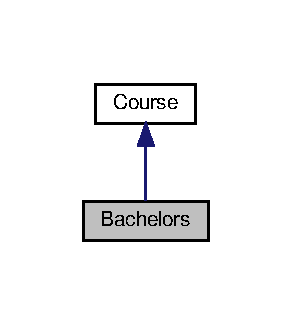
\includegraphics[width=140pt]{classBachelors__inherit__graph}
\end{center}
\end{figure}


Collaboration diagram for Bachelors\+:\nopagebreak
\begin{figure}[H]
\begin{center}
\leavevmode
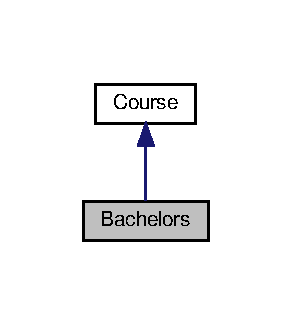
\includegraphics[width=140pt]{classBachelors__coll__graph}
\end{center}
\end{figure}
\subsection*{Public Member Functions}
\begin{DoxyCompactItemize}
\item 
\hyperlink{classBachelors_abc03be4ad19aaa51d5361e0aa4544618}{Bachelors} (unsigned int code, std\+::string name, std\+::map$<$ int, std\+::vector$<$ \hyperlink{classSubject}{Subject} $\ast$$>$$>$ curricular\+Plan, std\+::string director)
\item 
unsigned int \hyperlink{classBachelors_a08ab62391dbc677cabea2489e8da1889}{get\+Duration} () const
\item 
void \hyperlink{classBachelors_a25005e4fb6cfaddb749d13be04568c8b}{print\+Info} () const
\item 
void \hyperlink{classBachelors_adc2891e100ef21476e77efe6402e7580}{set\+Duration} (unsigned int d)
\item 
\mbox{\Hypertarget{classBachelors_a8cab815562dbb46b65975590792f3aae}\label{classBachelors_a8cab815562dbb46b65975590792f3aae}} 
void {\bfseries compated\+Information} (std\+::ofstream \&f)
\end{DoxyCompactItemize}
\subsection*{Additional Inherited Members}


\subsection{Detailed Description}


Definition at line 41 of file Course.\+hpp.



\subsection{Constructor \& Destructor Documentation}
\mbox{\Hypertarget{classBachelors_abc03be4ad19aaa51d5361e0aa4544618}\label{classBachelors_abc03be4ad19aaa51d5361e0aa4544618}} 
\index{Bachelors@{Bachelors}!Bachelors@{Bachelors}}
\index{Bachelors@{Bachelors}!Bachelors@{Bachelors}}
\subsubsection{\texorpdfstring{Bachelors()}{Bachelors()}}
{\footnotesize\ttfamily Bachelors\+::\+Bachelors (\begin{DoxyParamCaption}\item[{unsigned int}]{code,  }\item[{std\+::string}]{name,  }\item[{std\+::map$<$ int, std\+::vector$<$ \hyperlink{classSubject}{Subject} $\ast$$>$$>$}]{curricular\+Plan,  }\item[{std\+::string}]{director }\end{DoxyParamCaption})}

Constructs a \hyperlink{classBachelors}{Bachelors} objects with all the parameters. 
\begin{DoxyParams}{Parameters}
{\em code} & The code of the course. \\
\hline
{\em name} & The name of the course. \\
\hline
{\em curricular\+Plan} & The curricular plan of the course. \\
\hline
{\em director} & The director of the course. \\
\hline
\end{DoxyParams}


Definition at line 131 of file Course.\+cpp.



\subsection{Member Function Documentation}
\mbox{\Hypertarget{classBachelors_a08ab62391dbc677cabea2489e8da1889}\label{classBachelors_a08ab62391dbc677cabea2489e8da1889}} 
\index{Bachelors@{Bachelors}!get\+Duration@{get\+Duration}}
\index{get\+Duration@{get\+Duration}!Bachelors@{Bachelors}}
\subsubsection{\texorpdfstring{get\+Duration()}{getDuration()}}
{\footnotesize\ttfamily unsigned int Bachelors\+::get\+Duration (\begin{DoxyParamCaption}{ }\end{DoxyParamCaption}) const\hspace{0.3cm}{\ttfamily [virtual]}}

Gets the duration of the course. \begin{DoxyReturn}{Returns}
The duration of the course. 
\end{DoxyReturn}


Implements \hyperlink{classCourse}{Course}.



Definition at line 260 of file Course.\+cpp.

\mbox{\Hypertarget{classBachelors_a25005e4fb6cfaddb749d13be04568c8b}\label{classBachelors_a25005e4fb6cfaddb749d13be04568c8b}} 
\index{Bachelors@{Bachelors}!print\+Info@{print\+Info}}
\index{print\+Info@{print\+Info}!Bachelors@{Bachelors}}
\subsubsection{\texorpdfstring{print\+Info()}{printInfo()}}
{\footnotesize\ttfamily void Bachelors\+::print\+Info (\begin{DoxyParamCaption}{ }\end{DoxyParamCaption}) const\hspace{0.3cm}{\ttfamily [virtual]}}

Prints the values of the \hyperlink{classBachelors}{Bachelors}\textquotesingle{} class attributes. 

Reimplemented from \hyperlink{classCourse_a3248ecd5df196cf50ce379ec37758c59}{Course}.



Definition at line 142 of file Course.\+cpp.

Here is the call graph for this function\+:\nopagebreak
\begin{figure}[H]
\begin{center}
\leavevmode
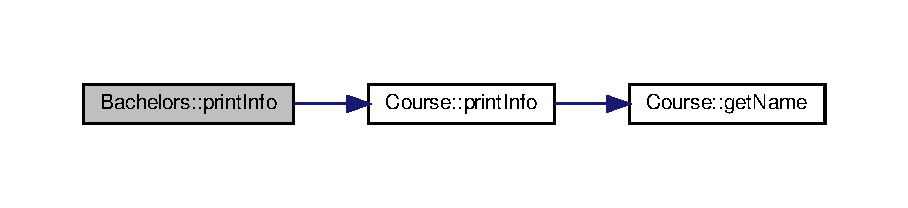
\includegraphics[width=350pt]{classBachelors_a25005e4fb6cfaddb749d13be04568c8b_cgraph}
\end{center}
\end{figure}
\mbox{\Hypertarget{classBachelors_adc2891e100ef21476e77efe6402e7580}\label{classBachelors_adc2891e100ef21476e77efe6402e7580}} 
\index{Bachelors@{Bachelors}!set\+Duration@{set\+Duration}}
\index{set\+Duration@{set\+Duration}!Bachelors@{Bachelors}}
\subsubsection{\texorpdfstring{set\+Duration()}{setDuration()}}
{\footnotesize\ttfamily void Bachelors\+::set\+Duration (\begin{DoxyParamCaption}\item[{unsigned int}]{d }\end{DoxyParamCaption})\hspace{0.3cm}{\ttfamily [virtual]}}

Sets the duration of the course. 
\begin{DoxyParams}{Parameters}
{\em d} & The duration of the course. \\
\hline
\end{DoxyParams}


Implements \hyperlink{classCourse}{Course}.



Definition at line 152 of file Course.\+cpp.



The documentation for this class was generated from the following files\+:\begin{DoxyCompactItemize}
\item 
include/Course.\+hpp\item 
src/Course.\+cpp\end{DoxyCompactItemize}

\hypertarget{classBinaryNode}{}\section{Binary\+Node$<$ Comparable $>$ Class Template Reference}
\label{classBinaryNode}\index{Binary\+Node$<$ Comparable $>$@{Binary\+Node$<$ Comparable $>$}}
\subsection*{Friends}
\begin{DoxyCompactItemize}
\item 
\mbox{\Hypertarget{classBinaryNode_a28a1adb9906f3ff7e12c2cb6fa2bd54e}\label{classBinaryNode_a28a1adb9906f3ff7e12c2cb6fa2bd54e}} 
class {\bfseries B\+S\+T$<$ Comparable $>$}
\item 
\mbox{\Hypertarget{classBinaryNode_aab3993acac2ab24a0b59edb0c3acc775}\label{classBinaryNode_aab3993acac2ab24a0b59edb0c3acc775}} 
class {\bfseries B\+S\+T\+Itr\+In$<$ Comparable $>$}
\item 
\mbox{\Hypertarget{classBinaryNode_a45a55df6f11541416d4ea7684c575c1a}\label{classBinaryNode_a45a55df6f11541416d4ea7684c575c1a}} 
class {\bfseries B\+S\+T\+Itr\+Pre$<$ Comparable $>$}
\item 
\mbox{\Hypertarget{classBinaryNode_a5dc153694be266f6e772659486219da7}\label{classBinaryNode_a5dc153694be266f6e772659486219da7}} 
class {\bfseries B\+S\+T\+Itr\+Post$<$ Comparable $>$}
\item 
\mbox{\Hypertarget{classBinaryNode_a26ff00bc0d87069aed877f10fd3c80a8}\label{classBinaryNode_a26ff00bc0d87069aed877f10fd3c80a8}} 
class {\bfseries B\+S\+T\+Itr\+Level$<$ Comparable $>$}
\end{DoxyCompactItemize}


\subsection{Detailed Description}
\subsubsection*{template$<$class Comparable$>$\newline
class Binary\+Node$<$ Comparable $>$}



Definition at line 27 of file B\+S\+T.\+h.



The documentation for this class was generated from the following file\+:\begin{DoxyCompactItemize}
\item 
include/B\+S\+T.\+h\end{DoxyCompactItemize}

\hypertarget{classBST}{}\section{B\+ST$<$ Comparable $>$ Class Template Reference}
\label{classBST}\index{B\+S\+T$<$ Comparable $>$@{B\+S\+T$<$ Comparable $>$}}
\subsection*{Public Member Functions}
\begin{DoxyCompactItemize}
\item 
\mbox{\Hypertarget{classBST_a3185a79cf472271f122a97d0f59022d1}\label{classBST_a3185a79cf472271f122a97d0f59022d1}} 
{\bfseries B\+ST} (const Comparable \&not\+Found)
\item 
\mbox{\Hypertarget{classBST_a163232cc6ffcbd1a51707efcc3fa36ca}\label{classBST_a163232cc6ffcbd1a51707efcc3fa36ca}} 
{\bfseries B\+ST} (const \hyperlink{classBST}{B\+ST} \&rhs)
\item 
\mbox{\Hypertarget{classBST_aa52491ff35aec517961937a17a9fa493}\label{classBST_aa52491ff35aec517961937a17a9fa493}} 
const Comparable \& {\bfseries find\+Min} () const
\item 
\mbox{\Hypertarget{classBST_a03485f3b0b150f1e69a12c28d26d8092}\label{classBST_a03485f3b0b150f1e69a12c28d26d8092}} 
const Comparable \& {\bfseries find\+Max} () const
\item 
\mbox{\Hypertarget{classBST_aaf4eb6869f68db0069534f7b2dfbe53b}\label{classBST_aaf4eb6869f68db0069534f7b2dfbe53b}} 
const Comparable \& {\bfseries find} (const Comparable \&x) const
\item 
\mbox{\Hypertarget{classBST_a10fd737b2be62437023407fdc123f728}\label{classBST_a10fd737b2be62437023407fdc123f728}} 
bool {\bfseries is\+Empty} () const
\item 
\mbox{\Hypertarget{classBST_a91e830925c48040d4c4dbb7d971c3bfe}\label{classBST_a91e830925c48040d4c4dbb7d971c3bfe}} 
void {\bfseries print\+Tree} () const
\item 
\mbox{\Hypertarget{classBST_a050d829503a88714c4ad0773cf6d3af6}\label{classBST_a050d829503a88714c4ad0773cf6d3af6}} 
void {\bfseries make\+Empty} ()
\item 
\mbox{\Hypertarget{classBST_a2b117df6521c7d61dac75ff2c938bae7}\label{classBST_a2b117df6521c7d61dac75ff2c938bae7}} 
void {\bfseries insert} (const Comparable \&x)
\item 
\mbox{\Hypertarget{classBST_a6f01a0b44daf82a42022b6eb4c0df7a2}\label{classBST_a6f01a0b44daf82a42022b6eb4c0df7a2}} 
void {\bfseries remove} (const Comparable \&x)
\item 
\mbox{\Hypertarget{classBST_aa80c39f454c89d4a202be3d1445823f3}\label{classBST_aa80c39f454c89d4a202be3d1445823f3}} 
const \hyperlink{classBST}{B\+ST} \& {\bfseries operator=} (const \hyperlink{classBST}{B\+ST} \&rhs)
\end{DoxyCompactItemize}
\subsection*{Friends}
\begin{DoxyCompactItemize}
\item 
\mbox{\Hypertarget{classBST_aab3993acac2ab24a0b59edb0c3acc775}\label{classBST_aab3993acac2ab24a0b59edb0c3acc775}} 
class {\bfseries B\+S\+T\+Itr\+In$<$ Comparable $>$}
\item 
\mbox{\Hypertarget{classBST_a45a55df6f11541416d4ea7684c575c1a}\label{classBST_a45a55df6f11541416d4ea7684c575c1a}} 
class {\bfseries B\+S\+T\+Itr\+Pre$<$ Comparable $>$}
\item 
\mbox{\Hypertarget{classBST_a5dc153694be266f6e772659486219da7}\label{classBST_a5dc153694be266f6e772659486219da7}} 
class {\bfseries B\+S\+T\+Itr\+Post$<$ Comparable $>$}
\item 
\mbox{\Hypertarget{classBST_a26ff00bc0d87069aed877f10fd3c80a8}\label{classBST_a26ff00bc0d87069aed877f10fd3c80a8}} 
class {\bfseries B\+S\+T\+Itr\+Level$<$ Comparable $>$}
\end{DoxyCompactItemize}


\subsection{Detailed Description}
\subsubsection*{template$<$class Comparable$>$\newline
class B\+S\+T$<$ Comparable $>$}



Definition at line 24 of file B\+S\+T.\+h.



The documentation for this class was generated from the following file\+:\begin{DoxyCompactItemize}
\item 
include/B\+S\+T.\+h\end{DoxyCompactItemize}

\hypertarget{classBSTItrIn}{}\section{B\+S\+T\+Itr\+In$<$ Comparable $>$ Class Template Reference}
\label{classBSTItrIn}\index{B\+S\+T\+Itr\+In$<$ Comparable $>$@{B\+S\+T\+Itr\+In$<$ Comparable $>$}}
\subsection*{Public Member Functions}
\begin{DoxyCompactItemize}
\item 
\mbox{\Hypertarget{classBSTItrIn_ac836e2f560fed9cc7ef8e5431a2836cc}\label{classBSTItrIn_ac836e2f560fed9cc7ef8e5431a2836cc}} 
{\bfseries B\+S\+T\+Itr\+In} (const \hyperlink{classBST}{B\+ST}$<$ Comparable $>$ \&bt)
\item 
\mbox{\Hypertarget{classBSTItrIn_ac772d3ebbac748c5f8cf9bc659f2e32c}\label{classBSTItrIn_ac772d3ebbac748c5f8cf9bc659f2e32c}} 
void {\bfseries advance} ()
\item 
\mbox{\Hypertarget{classBSTItrIn_a434375a2d263bf132ab3c4ac878af8ef}\label{classBSTItrIn_a434375a2d263bf132ab3c4ac878af8ef}} 
const Comparable \& {\bfseries retrieve} ()
\item 
\mbox{\Hypertarget{classBSTItrIn_a6f9a43217862c263a9bf15b9a08b889a}\label{classBSTItrIn_a6f9a43217862c263a9bf15b9a08b889a}} 
bool {\bfseries is\+At\+End} ()
\end{DoxyCompactItemize}


\subsection{Detailed Description}
\subsubsection*{template$<$class Comparable$>$\newline
class B\+S\+T\+Itr\+In$<$ Comparable $>$}



Definition at line 12 of file B\+S\+T.\+h.



The documentation for this class was generated from the following file\+:\begin{DoxyCompactItemize}
\item 
include/B\+S\+T.\+h\end{DoxyCompactItemize}

\hypertarget{classBSTItrLevel}{}\section{B\+S\+T\+Itr\+Level$<$ Comparable $>$ Class Template Reference}
\label{classBSTItrLevel}\index{B\+S\+T\+Itr\+Level$<$ Comparable $>$@{B\+S\+T\+Itr\+Level$<$ Comparable $>$}}
\subsection*{Public Member Functions}
\begin{DoxyCompactItemize}
\item 
\mbox{\Hypertarget{classBSTItrLevel_a8fd5cdde93eb182c4cd5cf6b2c5efaeb}\label{classBSTItrLevel_a8fd5cdde93eb182c4cd5cf6b2c5efaeb}} 
{\bfseries B\+S\+T\+Itr\+Level} (const \hyperlink{classBST}{B\+ST}$<$ Comparable $>$ \&bt)
\item 
\mbox{\Hypertarget{classBSTItrLevel_ad54a6fa289a59d6050b507abe40d463b}\label{classBSTItrLevel_ad54a6fa289a59d6050b507abe40d463b}} 
void {\bfseries advance} ()
\item 
\mbox{\Hypertarget{classBSTItrLevel_a7932a172129cc6ca14b6efeee1b4dd87}\label{classBSTItrLevel_a7932a172129cc6ca14b6efeee1b4dd87}} 
const Comparable \& {\bfseries retrieve} ()
\item 
\mbox{\Hypertarget{classBSTItrLevel_a89bc8e81dde255fd6bad917cacc0d489}\label{classBSTItrLevel_a89bc8e81dde255fd6bad917cacc0d489}} 
bool {\bfseries is\+At\+End} ()
\end{DoxyCompactItemize}


\subsection{Detailed Description}
\subsubsection*{template$<$class Comparable$>$\newline
class B\+S\+T\+Itr\+Level$<$ Comparable $>$}



Definition at line 21 of file B\+S\+T.\+h.



The documentation for this class was generated from the following file\+:\begin{DoxyCompactItemize}
\item 
include/B\+S\+T.\+h\end{DoxyCompactItemize}

\hypertarget{classBSTItrPost}{}\section{B\+S\+T\+Itr\+Post$<$ Comparable $>$ Class Template Reference}
\label{classBSTItrPost}\index{B\+S\+T\+Itr\+Post$<$ Comparable $>$@{B\+S\+T\+Itr\+Post$<$ Comparable $>$}}
\subsection*{Public Member Functions}
\begin{DoxyCompactItemize}
\item 
\mbox{\Hypertarget{classBSTItrPost_acf7e537dea01978f40c40909c55c56c2}\label{classBSTItrPost_acf7e537dea01978f40c40909c55c56c2}} 
{\bfseries B\+S\+T\+Itr\+Post} (const \hyperlink{classBST}{B\+ST}$<$ Comparable $>$ \&bt)
\item 
\mbox{\Hypertarget{classBSTItrPost_a376098e5a82cd02118dd4dcdec49bb26}\label{classBSTItrPost_a376098e5a82cd02118dd4dcdec49bb26}} 
void {\bfseries advance} ()
\item 
\mbox{\Hypertarget{classBSTItrPost_a1e9f3953f7ae5712bf3c7c6d05059718}\label{classBSTItrPost_a1e9f3953f7ae5712bf3c7c6d05059718}} 
const Comparable \& {\bfseries retrieve} ()
\item 
\mbox{\Hypertarget{classBSTItrPost_a2f330e73bb817e8bd1c797805e66ddb7}\label{classBSTItrPost_a2f330e73bb817e8bd1c797805e66ddb7}} 
bool {\bfseries is\+At\+End} ()
\end{DoxyCompactItemize}


\subsection{Detailed Description}
\subsubsection*{template$<$class Comparable$>$\newline
class B\+S\+T\+Itr\+Post$<$ Comparable $>$}



Definition at line 18 of file B\+S\+T.\+h.



The documentation for this class was generated from the following file\+:\begin{DoxyCompactItemize}
\item 
include/B\+S\+T.\+h\end{DoxyCompactItemize}

\hypertarget{classBSTItrPre}{}\section{B\+S\+T\+Itr\+Pre$<$ Comparable $>$ Class Template Reference}
\label{classBSTItrPre}\index{B\+S\+T\+Itr\+Pre$<$ Comparable $>$@{B\+S\+T\+Itr\+Pre$<$ Comparable $>$}}
\subsection*{Public Member Functions}
\begin{DoxyCompactItemize}
\item 
\mbox{\Hypertarget{classBSTItrPre_a11b1cd4e783f153b9c1b64ce2ec8077e}\label{classBSTItrPre_a11b1cd4e783f153b9c1b64ce2ec8077e}} 
{\bfseries B\+S\+T\+Itr\+Pre} (const \hyperlink{classBST}{B\+ST}$<$ Comparable $>$ \&bt)
\item 
\mbox{\Hypertarget{classBSTItrPre_a7a743d66a842018fd833fb2b0737254d}\label{classBSTItrPre_a7a743d66a842018fd833fb2b0737254d}} 
void {\bfseries advance} ()
\item 
\mbox{\Hypertarget{classBSTItrPre_ace3c36566d09f71eff8807c9a4fff7fe}\label{classBSTItrPre_ace3c36566d09f71eff8807c9a4fff7fe}} 
const Comparable \& {\bfseries retrieve} ()
\item 
\mbox{\Hypertarget{classBSTItrPre_ae282a7b9ffa9d250bb0f6a6d79f6e8d0}\label{classBSTItrPre_ae282a7b9ffa9d250bb0f6a6d79f6e8d0}} 
bool {\bfseries is\+At\+End} ()
\end{DoxyCompactItemize}


\subsection{Detailed Description}
\subsubsection*{template$<$class Comparable$>$\newline
class B\+S\+T\+Itr\+Pre$<$ Comparable $>$}



Definition at line 15 of file B\+S\+T.\+h.



The documentation for this class was generated from the following file\+:\begin{DoxyCompactItemize}
\item 
include/B\+S\+T.\+h\end{DoxyCompactItemize}

\hypertarget{classCourse}{}\section{Course Class Reference}
\label{classCourse}\index{Course@{Course}}


Inheritance diagram for Course\+:\nopagebreak
\begin{figure}[H]
\begin{center}
\leavevmode
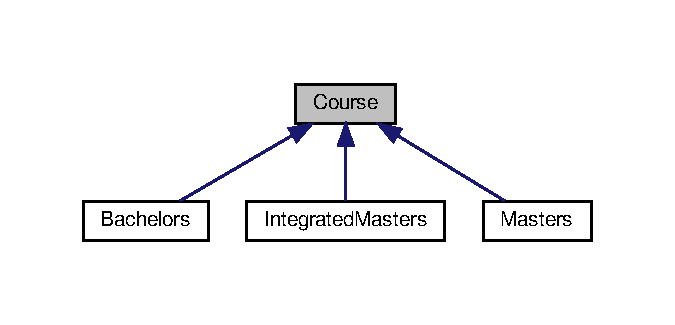
\includegraphics[width=324pt]{classCourse__inherit__graph}
\end{center}
\end{figure}
\subsection*{Public Member Functions}
\begin{DoxyCompactItemize}
\item 
\hyperlink{classCourse_a0caa544c52f7d2c69640be093d40f90b}{Course} (unsigned int code, std\+::string name, std\+::map$<$ int, std\+::vector$<$ \hyperlink{classSubject}{Subject} $\ast$$>$$>$ curricular\+Plan, std\+::string director)
\item 
virtual \hyperlink{classCourse_aa9038f2e129526920037dda9e76d69d0}{$\sim$\+Course} ()
\item 
unsigned int \hyperlink{classCourse_a6203b3564734a69d94779f168ff60ab5}{get\+Code} () const
\item 
std\+::string \hyperlink{classCourse_ab26b47d93027fcecffdf42b2ee526f87}{get\+Name} () const
\item 
std\+::map$<$ int, std\+::vector$<$ \hyperlink{classSubject}{Subject} $\ast$ $>$ $>$ \hyperlink{classCourse_a169989b538567685e25dcaf164b8e625}{get\+Curricular\+Plan} () const
\item 
std\+::string \hyperlink{classCourse_a604c801567695fc34bc932695a8943a0}{get\+Director} () const
\item 
\mbox{\Hypertarget{classCourse_af030e2cd407ebe7f390d554a62c0e333}\label{classCourse_af030e2cd407ebe7f390d554a62c0e333}} 
virtual unsigned int {\bfseries get\+Duration} () const =0
\item 
virtual void \hyperlink{classCourse_a3248ecd5df196cf50ce379ec37758c59}{print\+Info} () const
\item 
void \hyperlink{classCourse_a9bf594cc571e3cadd5d8df30c919bfa7}{set\+Name} (std\+::string name)
\item 
void \hyperlink{classCourse_a7aa38c1cf32c66b3c4307ff24d4e1f60}{set\+Code} (unsigned int code)
\item 
void \hyperlink{classCourse_a84a9fd9d25660d52a5b0f58b7d4383bc}{set\+Curricular\+Plan} (std\+::map$<$ int, std\+::vector$<$ \hyperlink{classSubject}{Subject} $\ast$$>$$>$ cp)
\item 
void \hyperlink{classCourse_a3b5489259ca31e4ffa2802dd84073b32}{set\+Director} (std\+::string director)
\item 
\mbox{\Hypertarget{classCourse_a416a700f90ee60d6ebaf1a99f3672deb}\label{classCourse_a416a700f90ee60d6ebaf1a99f3672deb}} 
virtual void {\bfseries set\+Duration} (unsigned int d)=0
\item 
void \hyperlink{classCourse_ac0ce13dcddfd17ccbd9606d0033aa713}{insert\+Year\+Subjects} (unsigned int year, vector$<$ \hyperlink{classSubject}{Subject} $\ast$$>$ subjects)
\item 
vector$<$ \hyperlink{classSubject}{Subject} $>$ \hyperlink{classCourse_a69d1fb52aa6c36851e0f6a8a5383de3d}{get\+Subjects} ()
\item 
void \hyperlink{classCourse_aa9b7e96bbf7689fe1b62d35b16bdc74f}{erase\+Subject} (\hyperlink{classSubject}{Subject} subject)
\item 
\mbox{\Hypertarget{classCourse_a43d77e0dd54f02a5e8a4e1840a669f9d}\label{classCourse_a43d77e0dd54f02a5e8a4e1840a669f9d}} 
virtual void {\bfseries compated\+Information} (std\+::ofstream \&f)=0
\end{DoxyCompactItemize}
\subsection*{Protected Attributes}
\begin{DoxyCompactItemize}
\item 
\mbox{\Hypertarget{classCourse_ab5286ae7c73c3dd66c3a99f630c17c0a}\label{classCourse_ab5286ae7c73c3dd66c3a99f630c17c0a}} 
std\+::string {\bfseries name}
\item 
\mbox{\Hypertarget{classCourse_a04d959210c3d7a4fbb4a66c260419c6d}\label{classCourse_a04d959210c3d7a4fbb4a66c260419c6d}} 
unsigned int {\bfseries code}
\item 
\mbox{\Hypertarget{classCourse_a5df6b76f92fe29c6521262afc4214103}\label{classCourse_a5df6b76f92fe29c6521262afc4214103}} 
std\+::map$<$ int, std\+::vector$<$ \hyperlink{classSubject}{Subject} $\ast$ $>$ $>$ {\bfseries curricular\+Plan}
\item 
\mbox{\Hypertarget{classCourse_a07f2b89a7c5e9667651671f41f8e1219}\label{classCourse_a07f2b89a7c5e9667651671f41f8e1219}} 
std\+::string {\bfseries director}
\end{DoxyCompactItemize}


\subsection{Detailed Description}


Definition at line 10 of file Course.\+hpp.



\subsection{Constructor \& Destructor Documentation}
\mbox{\Hypertarget{classCourse_a0caa544c52f7d2c69640be093d40f90b}\label{classCourse_a0caa544c52f7d2c69640be093d40f90b}} 
\index{Course@{Course}!Course@{Course}}
\index{Course@{Course}!Course@{Course}}
\subsubsection{\texorpdfstring{Course()}{Course()}}
{\footnotesize\ttfamily Course\+::\+Course (\begin{DoxyParamCaption}\item[{unsigned int}]{code,  }\item[{std\+::string}]{name,  }\item[{std\+::map$<$ int, std\+::vector$<$ \hyperlink{classSubject}{Subject} $\ast$$>$$>$}]{curricular\+Plan,  }\item[{std\+::string}]{director }\end{DoxyParamCaption})}

Constructs a \hyperlink{classCourse}{Course} object with all parameters. 
\begin{DoxyParams}{Parameters}
{\em code} & The code of the course \\
\hline
{\em name} & The name of the course \\
\hline
{\em curricular\+Plan} & The curricular plan of the course \\
\hline
{\em director} & The director of the course \\
\hline
\end{DoxyParams}


Definition at line 10 of file Course.\+cpp.

\mbox{\Hypertarget{classCourse_aa9038f2e129526920037dda9e76d69d0}\label{classCourse_aa9038f2e129526920037dda9e76d69d0}} 
\index{Course@{Course}!````~Course@{$\sim$\+Course}}
\index{````~Course@{$\sim$\+Course}!Course@{Course}}
\subsubsection{\texorpdfstring{$\sim$\+Course()}{~Course()}}
{\footnotesize\ttfamily Course\+::$\sim$\+Course (\begin{DoxyParamCaption}{ }\end{DoxyParamCaption})\hspace{0.3cm}{\ttfamily [virtual]}}

Destructs a \hyperlink{classCourse}{Course} object. 

Definition at line 32 of file Course.\+cpp.



\subsection{Member Function Documentation}
\mbox{\Hypertarget{classCourse_aa9b7e96bbf7689fe1b62d35b16bdc74f}\label{classCourse_aa9b7e96bbf7689fe1b62d35b16bdc74f}} 
\index{Course@{Course}!erase\+Subject@{erase\+Subject}}
\index{erase\+Subject@{erase\+Subject}!Course@{Course}}
\subsubsection{\texorpdfstring{erase\+Subject()}{eraseSubject()}}
{\footnotesize\ttfamily void Course\+::erase\+Subject (\begin{DoxyParamCaption}\item[{\hyperlink{classSubject}{Subject}}]{subject }\end{DoxyParamCaption})}

Erases a subject from the course. 
\begin{DoxyParams}{Parameters}
{\em subject} & A subject of the course. \\
\hline
\end{DoxyParams}


Definition at line 306 of file Course.\+cpp.

\mbox{\Hypertarget{classCourse_a6203b3564734a69d94779f168ff60ab5}\label{classCourse_a6203b3564734a69d94779f168ff60ab5}} 
\index{Course@{Course}!get\+Code@{get\+Code}}
\index{get\+Code@{get\+Code}!Course@{Course}}
\subsubsection{\texorpdfstring{get\+Code()}{getCode()}}
{\footnotesize\ttfamily unsigned int Course\+::get\+Code (\begin{DoxyParamCaption}{ }\end{DoxyParamCaption}) const}

Gets the code of the course. \begin{DoxyReturn}{Returns}
The code of the course. 
\end{DoxyReturn}


Definition at line 225 of file Course.\+cpp.

\mbox{\Hypertarget{classCourse_a169989b538567685e25dcaf164b8e625}\label{classCourse_a169989b538567685e25dcaf164b8e625}} 
\index{Course@{Course}!get\+Curricular\+Plan@{get\+Curricular\+Plan}}
\index{get\+Curricular\+Plan@{get\+Curricular\+Plan}!Course@{Course}}
\subsubsection{\texorpdfstring{get\+Curricular\+Plan()}{getCurricularPlan()}}
{\footnotesize\ttfamily std\+::map$<$ int, std\+::vector$<$ \hyperlink{classSubject}{Subject} $\ast$ $>$ $>$ Course\+::get\+Curricular\+Plan (\begin{DoxyParamCaption}{ }\end{DoxyParamCaption}) const}

Gets the curricular plan of the course. \begin{DoxyReturn}{Returns}
The curricular plan of the course. 
\end{DoxyReturn}


Definition at line 243 of file Course.\+cpp.

\mbox{\Hypertarget{classCourse_a604c801567695fc34bc932695a8943a0}\label{classCourse_a604c801567695fc34bc932695a8943a0}} 
\index{Course@{Course}!get\+Director@{get\+Director}}
\index{get\+Director@{get\+Director}!Course@{Course}}
\subsubsection{\texorpdfstring{get\+Director()}{getDirector()}}
{\footnotesize\ttfamily std\+::string Course\+::get\+Director (\begin{DoxyParamCaption}{ }\end{DoxyParamCaption}) const}

Gets the director of the course. \begin{DoxyReturn}{Returns}
The director of the course. 
\end{DoxyReturn}


Definition at line 251 of file Course.\+cpp.

\mbox{\Hypertarget{classCourse_ab26b47d93027fcecffdf42b2ee526f87}\label{classCourse_ab26b47d93027fcecffdf42b2ee526f87}} 
\index{Course@{Course}!get\+Name@{get\+Name}}
\index{get\+Name@{get\+Name}!Course@{Course}}
\subsubsection{\texorpdfstring{get\+Name()}{getName()}}
{\footnotesize\ttfamily std\+::string Course\+::get\+Name (\begin{DoxyParamCaption}{ }\end{DoxyParamCaption}) const}

Gets the name of the course. \begin{DoxyReturn}{Returns}
The name of the course. 
\end{DoxyReturn}


Definition at line 234 of file Course.\+cpp.

\mbox{\Hypertarget{classCourse_a69d1fb52aa6c36851e0f6a8a5383de3d}\label{classCourse_a69d1fb52aa6c36851e0f6a8a5383de3d}} 
\index{Course@{Course}!get\+Subjects@{get\+Subjects}}
\index{get\+Subjects@{get\+Subjects}!Course@{Course}}
\subsubsection{\texorpdfstring{get\+Subjects()}{getSubjects()}}
{\footnotesize\ttfamily vector$<$ \hyperlink{classSubject}{Subject} $>$ Course\+::get\+Subjects (\begin{DoxyParamCaption}{ }\end{DoxyParamCaption})}

Gets every subjec of the course. \begin{DoxyReturn}{Returns}
Every subject of the course. 
\end{DoxyReturn}


Definition at line 287 of file Course.\+cpp.

\mbox{\Hypertarget{classCourse_ac0ce13dcddfd17ccbd9606d0033aa713}\label{classCourse_ac0ce13dcddfd17ccbd9606d0033aa713}} 
\index{Course@{Course}!insert\+Year\+Subjects@{insert\+Year\+Subjects}}
\index{insert\+Year\+Subjects@{insert\+Year\+Subjects}!Course@{Course}}
\subsubsection{\texorpdfstring{insert\+Year\+Subjects()}{insertYearSubjects()}}
{\footnotesize\ttfamily void Course\+::insert\+Year\+Subjects (\begin{DoxyParamCaption}\item[{unsigned int}]{year,  }\item[{vector$<$ \hyperlink{classSubject}{Subject} $\ast$$>$}]{subjects }\end{DoxyParamCaption})}

Inserts a number of subjects into the respective curricular year. 
\begin{DoxyParams}{Parameters}
{\em year} & The curricular year. \\
\hline
{\em subjects} & The subjects to be inserted. \\
\hline
\end{DoxyParams}


Definition at line 107 of file Course.\+cpp.

\mbox{\Hypertarget{classCourse_a3248ecd5df196cf50ce379ec37758c59}\label{classCourse_a3248ecd5df196cf50ce379ec37758c59}} 
\index{Course@{Course}!print\+Info@{print\+Info}}
\index{print\+Info@{print\+Info}!Course@{Course}}
\subsubsection{\texorpdfstring{print\+Info()}{printInfo()}}
{\footnotesize\ttfamily void Course\+::print\+Info (\begin{DoxyParamCaption}{ }\end{DoxyParamCaption}) const\hspace{0.3cm}{\ttfamily [virtual]}}

Prints the information of a \hyperlink{classCourse}{Course} object. Every atribuite of the class\textquotesingle{}s object is printed. 

Reimplemented in \hyperlink{classIntegratedMasters_a71d4f5089e42207af1106604e316f155}{Integrated\+Masters}, \hyperlink{classMasters_a72034d4ad86c3d62c755ad04228d09da}{Masters}, and \hyperlink{classBachelors_a25005e4fb6cfaddb749d13be04568c8b}{Bachelors}.



Definition at line 48 of file Course.\+cpp.

Here is the call graph for this function\+:\nopagebreak
\begin{figure}[H]
\begin{center}
\leavevmode
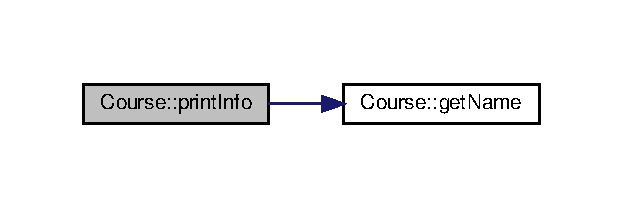
\includegraphics[width=299pt]{classCourse_a3248ecd5df196cf50ce379ec37758c59_cgraph}
\end{center}
\end{figure}
\mbox{\Hypertarget{classCourse_a7aa38c1cf32c66b3c4307ff24d4e1f60}\label{classCourse_a7aa38c1cf32c66b3c4307ff24d4e1f60}} 
\index{Course@{Course}!set\+Code@{set\+Code}}
\index{set\+Code@{set\+Code}!Course@{Course}}
\subsubsection{\texorpdfstring{set\+Code()}{setCode()}}
{\footnotesize\ttfamily void Course\+::set\+Code (\begin{DoxyParamCaption}\item[{unsigned int}]{code }\end{DoxyParamCaption})}

Sets the code of a \hyperlink{classCourse}{Course} object. 
\begin{DoxyParams}{Parameters}
{\em code} & The code of the course. \\
\hline
\end{DoxyParams}


Definition at line 79 of file Course.\+cpp.

\mbox{\Hypertarget{classCourse_a84a9fd9d25660d52a5b0f58b7d4383bc}\label{classCourse_a84a9fd9d25660d52a5b0f58b7d4383bc}} 
\index{Course@{Course}!set\+Curricular\+Plan@{set\+Curricular\+Plan}}
\index{set\+Curricular\+Plan@{set\+Curricular\+Plan}!Course@{Course}}
\subsubsection{\texorpdfstring{set\+Curricular\+Plan()}{setCurricularPlan()}}
{\footnotesize\ttfamily void Course\+::set\+Curricular\+Plan (\begin{DoxyParamCaption}\item[{std\+::map$<$ int, std\+::vector$<$ \hyperlink{classSubject}{Subject} $\ast$$>$$>$}]{cp }\end{DoxyParamCaption})}

Sets the curricular plan of the course. 
\begin{DoxyParams}{Parameters}
{\em cp} & The curricular plan of the course. \\
\hline
\end{DoxyParams}


Definition at line 88 of file Course.\+cpp.

\mbox{\Hypertarget{classCourse_a3b5489259ca31e4ffa2802dd84073b32}\label{classCourse_a3b5489259ca31e4ffa2802dd84073b32}} 
\index{Course@{Course}!set\+Director@{set\+Director}}
\index{set\+Director@{set\+Director}!Course@{Course}}
\subsubsection{\texorpdfstring{set\+Director()}{setDirector()}}
{\footnotesize\ttfamily void Course\+::set\+Director (\begin{DoxyParamCaption}\item[{std\+::string}]{director }\end{DoxyParamCaption})}

Sets the director of the course. 
\begin{DoxyParams}{Parameters}
{\em director} & The director of the course. \\
\hline
\end{DoxyParams}


Definition at line 97 of file Course.\+cpp.

\mbox{\Hypertarget{classCourse_a9bf594cc571e3cadd5d8df30c919bfa7}\label{classCourse_a9bf594cc571e3cadd5d8df30c919bfa7}} 
\index{Course@{Course}!set\+Name@{set\+Name}}
\index{set\+Name@{set\+Name}!Course@{Course}}
\subsubsection{\texorpdfstring{set\+Name()}{setName()}}
{\footnotesize\ttfamily void Course\+::set\+Name (\begin{DoxyParamCaption}\item[{std\+::string}]{name }\end{DoxyParamCaption})}

Sets the name of a \hyperlink{classCourse}{Course} object. 
\begin{DoxyParams}{Parameters}
{\em name} & The name of the course. \\
\hline
\end{DoxyParams}


Definition at line 70 of file Course.\+cpp.



The documentation for this class was generated from the following files\+:\begin{DoxyCompactItemize}
\item 
include/Course.\+hpp\item 
src/Course.\+cpp\end{DoxyCompactItemize}

\hypertarget{classDate}{}\section{Date Class Reference}
\label{classDate}\index{Date@{Date}}
\subsection*{Public Member Functions}
\begin{DoxyCompactItemize}
\item 
\hyperlink{classDate_a28c6604a0f8ed8216becf24abc20cf5b}{Date} (unsigned int day, unsigned int month, unsigned int year)
\item 
unsigned int \hyperlink{classDate_a9efc6db1870de82dbd717f1c3c782f82}{get\+Month} ()
\item 
unsigned int \hyperlink{classDate_a90be6a509b91ee9addfeec0e68b965e2}{get\+Year} ()
\item 
unsigned int \hyperlink{classDate_ab39b571a45cbcdfd37b23c28801fa7b0}{get\+Day} ()
\item 
void \hyperlink{classDate_a18dc2bd52ab8adcca331f66c27ed6623}{set\+Day} (unsigned int day)
\item 
void \hyperlink{classDate_aa83b79359070012ab58ff99abeb34340}{set\+Month} (unsigned int month)
\item 
void \hyperlink{classDate_a895c4ae9868e43577cf59d9c679d7a71}{set\+Year} (int year)
\item 
void \hyperlink{classDate_a6d5873842b1ede5d95399220d7994c7b}{print\+Date} () const
\item 
bool \hyperlink{classDate_a2fdc0ec866aa7e1b3f8e1a7468663827}{operator$<$} (\hyperlink{classDate}{Date} d1) const
\item 
bool \hyperlink{classDate_aa71c76d80b90438a9b507e8fba4beaa4}{operator$>$} (\hyperlink{classDate}{Date} d1) const
\item 
\mbox{\Hypertarget{classDate_afc8db375619a48b87cd267e801cc2230}\label{classDate_afc8db375619a48b87cd267e801cc2230}} 
string {\bfseries to\+String} ()
\end{DoxyCompactItemize}


\subsection{Detailed Description}


Definition at line 9 of file Date.\+hpp.



\subsection{Constructor \& Destructor Documentation}
\mbox{\Hypertarget{classDate_a28c6604a0f8ed8216becf24abc20cf5b}\label{classDate_a28c6604a0f8ed8216becf24abc20cf5b}} 
\index{Date@{Date}!Date@{Date}}
\index{Date@{Date}!Date@{Date}}
\subsubsection{\texorpdfstring{Date()}{Date()}}
{\footnotesize\ttfamily Date\+::\+Date (\begin{DoxyParamCaption}\item[{unsigned int}]{day,  }\item[{unsigned int}]{month,  }\item[{unsigned int}]{year }\end{DoxyParamCaption})}

Constructs an object of type \hyperlink{classDate}{Date}. 
\begin{DoxyParams}{Parameters}
{\em day} & The day of the date. \\
\hline
{\em month} & The month of the date. \\
\hline
{\em year} & The year of the date. \\
\hline
\end{DoxyParams}


Definition at line 70 of file Date.\+cpp.

Here is the call graph for this function\+:\nopagebreak
\begin{figure}[H]
\begin{center}
\leavevmode
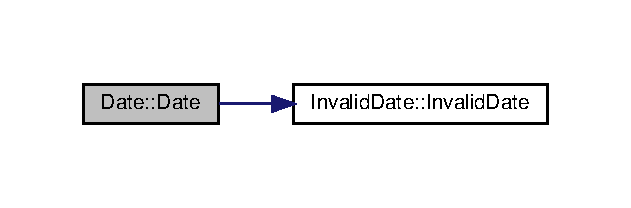
\includegraphics[width=303pt]{classDate_a28c6604a0f8ed8216becf24abc20cf5b_cgraph}
\end{center}
\end{figure}


\subsection{Member Function Documentation}
\mbox{\Hypertarget{classDate_ab39b571a45cbcdfd37b23c28801fa7b0}\label{classDate_ab39b571a45cbcdfd37b23c28801fa7b0}} 
\index{Date@{Date}!get\+Day@{get\+Day}}
\index{get\+Day@{get\+Day}!Date@{Date}}
\subsubsection{\texorpdfstring{get\+Day()}{getDay()}}
{\footnotesize\ttfamily unsigned int Date\+::get\+Day (\begin{DoxyParamCaption}{ }\end{DoxyParamCaption})}

Gets the day of the date. \begin{DoxyReturn}{Returns}

\end{DoxyReturn}


Definition at line 120 of file Date.\+cpp.

\mbox{\Hypertarget{classDate_a9efc6db1870de82dbd717f1c3c782f82}\label{classDate_a9efc6db1870de82dbd717f1c3c782f82}} 
\index{Date@{Date}!get\+Month@{get\+Month}}
\index{get\+Month@{get\+Month}!Date@{Date}}
\subsubsection{\texorpdfstring{get\+Month()}{getMonth()}}
{\footnotesize\ttfamily unsigned int Date\+::get\+Month (\begin{DoxyParamCaption}{ }\end{DoxyParamCaption})}

Gets the month of the date. \begin{DoxyReturn}{Returns}

\end{DoxyReturn}


Definition at line 111 of file Date.\+cpp.

\mbox{\Hypertarget{classDate_a90be6a509b91ee9addfeec0e68b965e2}\label{classDate_a90be6a509b91ee9addfeec0e68b965e2}} 
\index{Date@{Date}!get\+Year@{get\+Year}}
\index{get\+Year@{get\+Year}!Date@{Date}}
\subsubsection{\texorpdfstring{get\+Year()}{getYear()}}
{\footnotesize\ttfamily unsigned int Date\+::get\+Year (\begin{DoxyParamCaption}{ }\end{DoxyParamCaption})}

Gets the year of the date. \begin{DoxyReturn}{Returns}

\end{DoxyReturn}


Definition at line 102 of file Date.\+cpp.

\mbox{\Hypertarget{classDate_a2fdc0ec866aa7e1b3f8e1a7468663827}\label{classDate_a2fdc0ec866aa7e1b3f8e1a7468663827}} 
\index{Date@{Date}!operator$<$@{operator$<$}}
\index{operator$<$@{operator$<$}!Date@{Date}}
\subsubsection{\texorpdfstring{operator$<$()}{operator<()}}
{\footnotesize\ttfamily bool Date\+::operator$<$ (\begin{DoxyParamCaption}\item[{\hyperlink{classDate}{Date}}]{d1 }\end{DoxyParamCaption}) const}

Compares if one date is smaller than the other 
\begin{DoxyParams}{Parameters}
{\em d1} & A date to be used in the comparison \\
\hline
\end{DoxyParams}
\begin{DoxyReturn}{Returns}
The smallest date 
\end{DoxyReturn}


Definition at line 186 of file Date.\+cpp.

\mbox{\Hypertarget{classDate_aa71c76d80b90438a9b507e8fba4beaa4}\label{classDate_aa71c76d80b90438a9b507e8fba4beaa4}} 
\index{Date@{Date}!operator$>$@{operator$>$}}
\index{operator$>$@{operator$>$}!Date@{Date}}
\subsubsection{\texorpdfstring{operator$>$()}{operator>()}}
{\footnotesize\ttfamily bool Date\+::operator$>$ (\begin{DoxyParamCaption}\item[{\hyperlink{classDate}{Date}}]{d1 }\end{DoxyParamCaption}) const}

Compares if one date is bigger than the other 
\begin{DoxyParams}{Parameters}
{\em d1} & A date to be used in the comparison \\
\hline
\end{DoxyParams}
\begin{DoxyReturn}{Returns}
The biggest date 
\end{DoxyReturn}


Definition at line 206 of file Date.\+cpp.

\mbox{\Hypertarget{classDate_a6d5873842b1ede5d95399220d7994c7b}\label{classDate_a6d5873842b1ede5d95399220d7994c7b}} 
\index{Date@{Date}!print\+Date@{print\+Date}}
\index{print\+Date@{print\+Date}!Date@{Date}}
\subsubsection{\texorpdfstring{print\+Date()}{printDate()}}
{\footnotesize\ttfamily void Date\+::print\+Date (\begin{DoxyParamCaption}{ }\end{DoxyParamCaption}) const}

Prints the date in the format dd/mm/yyyy. 

Definition at line 128 of file Date.\+cpp.

\mbox{\Hypertarget{classDate_a18dc2bd52ab8adcca331f66c27ed6623}\label{classDate_a18dc2bd52ab8adcca331f66c27ed6623}} 
\index{Date@{Date}!set\+Day@{set\+Day}}
\index{set\+Day@{set\+Day}!Date@{Date}}
\subsubsection{\texorpdfstring{set\+Day()}{setDay()}}
{\footnotesize\ttfamily void Date\+::set\+Day (\begin{DoxyParamCaption}\item[{unsigned int}]{day }\end{DoxyParamCaption})}

Sets the day of the date. 
\begin{DoxyParams}{Parameters}
{\em day} & The day of the date. \\
\hline
\end{DoxyParams}


Definition at line 137 of file Date.\+cpp.

Here is the call graph for this function\+:\nopagebreak
\begin{figure}[H]
\begin{center}
\leavevmode
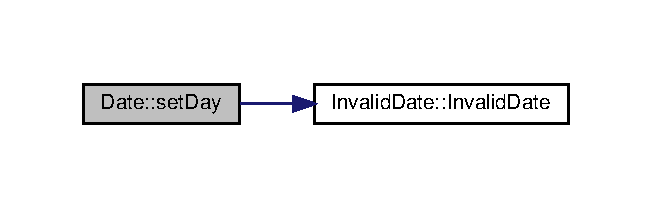
\includegraphics[width=313pt]{classDate_a18dc2bd52ab8adcca331f66c27ed6623_cgraph}
\end{center}
\end{figure}
\mbox{\Hypertarget{classDate_aa83b79359070012ab58ff99abeb34340}\label{classDate_aa83b79359070012ab58ff99abeb34340}} 
\index{Date@{Date}!set\+Month@{set\+Month}}
\index{set\+Month@{set\+Month}!Date@{Date}}
\subsubsection{\texorpdfstring{set\+Month()}{setMonth()}}
{\footnotesize\ttfamily void Date\+::set\+Month (\begin{DoxyParamCaption}\item[{unsigned int}]{month }\end{DoxyParamCaption})}

Sets the month of the date. 
\begin{DoxyParams}{Parameters}
{\em month} & The month of the date. \\
\hline
\end{DoxyParams}


Definition at line 153 of file Date.\+cpp.

Here is the call graph for this function\+:\nopagebreak
\begin{figure}[H]
\begin{center}
\leavevmode
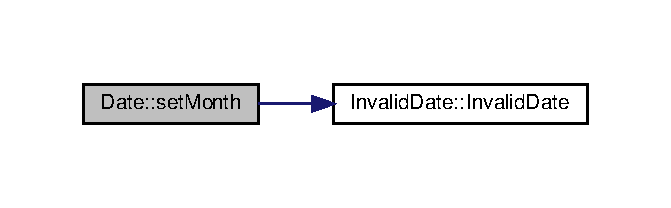
\includegraphics[width=322pt]{classDate_aa83b79359070012ab58ff99abeb34340_cgraph}
\end{center}
\end{figure}
\mbox{\Hypertarget{classDate_a895c4ae9868e43577cf59d9c679d7a71}\label{classDate_a895c4ae9868e43577cf59d9c679d7a71}} 
\index{Date@{Date}!set\+Year@{set\+Year}}
\index{set\+Year@{set\+Year}!Date@{Date}}
\subsubsection{\texorpdfstring{set\+Year()}{setYear()}}
{\footnotesize\ttfamily void Date\+::set\+Year (\begin{DoxyParamCaption}\item[{int}]{year }\end{DoxyParamCaption})}

Sets the year of the date. 
\begin{DoxyParams}{Parameters}
{\em year} & The year of the date. \\
\hline
\end{DoxyParams}


Definition at line 169 of file Date.\+cpp.

Here is the call graph for this function\+:\nopagebreak
\begin{figure}[H]
\begin{center}
\leavevmode
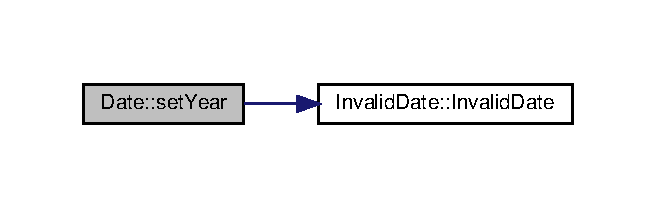
\includegraphics[width=315pt]{classDate_a895c4ae9868e43577cf59d9c679d7a71_cgraph}
\end{center}
\end{figure}


The documentation for this class was generated from the following files\+:\begin{DoxyCompactItemize}
\item 
include/Date.\+hpp\item 
src/Date.\+cpp\end{DoxyCompactItemize}

\hypertarget{classDepartment}{}\section{Department Class Reference}
\label{classDepartment}\index{Department@{Department}}
\subsection*{Public Member Functions}
\begin{DoxyCompactItemize}
\item 
\hyperlink{classDepartment_a9d85b4973d29f519e09fdafa53a56e8c}{Department} ()
\item 
\hyperlink{classDepartment_a75a594311b114c794be126f5e2cd6a2d}{Department} (std\+::string name, std\+::vector$<$ \hyperlink{classCourse}{Course} $\ast$$>$ courses)
\item 
\hyperlink{classDepartment_a15f5619c6679ffc80fe6de41c7a2e4a1}{$\sim$\+Department} ()
\item 
std\+::string \hyperlink{classDepartment_a3ada89e70eae97b429c9a82f601e98c0}{get\+Name} () const
\item 
std\+::vector$<$ \hyperlink{classCourse}{Course} $\ast$ $>$ \hyperlink{classDepartment_a1a350298618bf4be8cc42eabef377212}{get\+Courses} () const
\item 
void \hyperlink{classDepartment_a020f24af6978f0033895e8ebde27bbfb}{sort\+\_\+courses\+\_\+name\+\_\+crescent} ()
\item 
void \hyperlink{classDepartment_a7798d17dd46c0859cf6ce68c7ec434ae}{sort\+\_\+courses\+\_\+name\+\_\+decrescent} ()
\item 
void \hyperlink{classDepartment_accf36d58f8b5e8110148f3a69ad30278}{sort\+\_\+courses\+\_\+code\+\_\+crescent} ()
\item 
void \hyperlink{classDepartment_a320c23411a02eba00f00a15895c538b2}{sort\+\_\+courses\+\_\+code\+\_\+decrescent} ()
\item 
void \hyperlink{classDepartment_ab15a7312cdf65f53c3796c428bb6211b}{print\+Info} () const
\item 
void \hyperlink{classDepartment_adbde303b8c83a10b3da68ee9f949f731}{set\+Name} (std\+::string name)
\item 
void \hyperlink{classDepartment_a52742b6ce155016eb084ccd2faccdeef}{set\+Courses} (std\+::vector$<$ \hyperlink{classCourse}{Course} $\ast$$>$ courses)
\item 
void \hyperlink{classDepartment_a93ca2b0446a426603f62786693c57b47}{add\+Course} (\hyperlink{classCourse}{Course} $\ast$course)
\item 
void \hyperlink{classDepartment_a01acd70fa3c49ebe0d729a910c842078}{erase\+Course} (\hyperlink{classCourse}{Course} $\ast$course)
\item 
\hyperlink{classCourse}{Course} $\ast$ \hyperlink{classDepartment_a2f776e8ddcf895cccdf60beb206b8620}{find\+\_\+course\+\_\+by\+\_\+name} (std\+::string name) const
\item 
\hyperlink{classCourse}{Course} $\ast$ \hyperlink{classDepartment_af8e8a8aa806e5925c07686cadd70fde2}{find\+\_\+course\+\_\+by\+\_\+code} (unsigned int code) const
\item 
\hyperlink{classCourse}{Course} $\ast$ \hyperlink{classDepartment_a5d83db657bd838d17ac04be757f887a5}{find\+\_\+course\+\_\+by\+\_\+director} (std\+::string director) const
\item 
\mbox{\Hypertarget{classDepartment_abbfb590bf8b197e23837f1c932a1c278}\label{classDepartment_abbfb590bf8b197e23837f1c932a1c278}} 
void {\bfseries compated\+Information} (std\+::ofstream \&f)
\end{DoxyCompactItemize}


\subsection{Detailed Description}


Definition at line 8 of file Department.\+hpp.



\subsection{Constructor \& Destructor Documentation}
\mbox{\Hypertarget{classDepartment_a9d85b4973d29f519e09fdafa53a56e8c}\label{classDepartment_a9d85b4973d29f519e09fdafa53a56e8c}} 
\index{Department@{Department}!Department@{Department}}
\index{Department@{Department}!Department@{Department}}
\subsubsection{\texorpdfstring{Department()}{Department()}\hspace{0.1cm}{\footnotesize\ttfamily [1/2]}}
{\footnotesize\ttfamily Department\+::\+Department (\begin{DoxyParamCaption}{ }\end{DoxyParamCaption})}

Constructs an empty \hyperlink{classDepartment}{Department} object. 

Definition at line 22 of file Department.\+cpp.

\mbox{\Hypertarget{classDepartment_a75a594311b114c794be126f5e2cd6a2d}\label{classDepartment_a75a594311b114c794be126f5e2cd6a2d}} 
\index{Department@{Department}!Department@{Department}}
\index{Department@{Department}!Department@{Department}}
\subsubsection{\texorpdfstring{Department()}{Department()}\hspace{0.1cm}{\footnotesize\ttfamily [2/2]}}
{\footnotesize\ttfamily Department\+::\+Department (\begin{DoxyParamCaption}\item[{std\+::string}]{name,  }\item[{std\+::vector$<$ \hyperlink{classCourse}{Course} $\ast$$>$}]{courses }\end{DoxyParamCaption})}

Constructs a \hyperlink{classDepartment}{Department} object. 
\begin{DoxyParams}{Parameters}
{\em name} & The name of the department. \\
\hline
{\em courses} & The courses of the department. \\
\hline
\end{DoxyParams}


Definition at line 8 of file Department.\+cpp.

\mbox{\Hypertarget{classDepartment_a15f5619c6679ffc80fe6de41c7a2e4a1}\label{classDepartment_a15f5619c6679ffc80fe6de41c7a2e4a1}} 
\index{Department@{Department}!````~Department@{$\sim$\+Department}}
\index{````~Department@{$\sim$\+Department}!Department@{Department}}
\subsubsection{\texorpdfstring{$\sim$\+Department()}{~Department()}}
{\footnotesize\ttfamily Department\+::$\sim$\+Department (\begin{DoxyParamCaption}{ }\end{DoxyParamCaption})}

Destroys a \hyperlink{classDepartment}{Department} object. 

Definition at line 27 of file Department.\+cpp.



\subsection{Member Function Documentation}
\mbox{\Hypertarget{classDepartment_a93ca2b0446a426603f62786693c57b47}\label{classDepartment_a93ca2b0446a426603f62786693c57b47}} 
\index{Department@{Department}!add\+Course@{add\+Course}}
\index{add\+Course@{add\+Course}!Department@{Department}}
\subsubsection{\texorpdfstring{add\+Course()}{addCourse()}}
{\footnotesize\ttfamily void Department\+::add\+Course (\begin{DoxyParamCaption}\item[{\hyperlink{classCourse}{Course} $\ast$}]{course }\end{DoxyParamCaption})}

Adds a course to the departent. 
\begin{DoxyParams}{Parameters}
{\em course} & A course. \\
\hline
\end{DoxyParams}


Definition at line 89 of file Department.\+cpp.

\mbox{\Hypertarget{classDepartment_a01acd70fa3c49ebe0d729a910c842078}\label{classDepartment_a01acd70fa3c49ebe0d729a910c842078}} 
\index{Department@{Department}!erase\+Course@{erase\+Course}}
\index{erase\+Course@{erase\+Course}!Department@{Department}}
\subsubsection{\texorpdfstring{erase\+Course()}{eraseCourse()}}
{\footnotesize\ttfamily void Department\+::erase\+Course (\begin{DoxyParamCaption}\item[{\hyperlink{classCourse}{Course} $\ast$}]{course }\end{DoxyParamCaption})}

Erases a course from the vector of courses. 
\begin{DoxyParams}{Parameters}
{\em course} & A course. \\
\hline
\end{DoxyParams}


Definition at line 98 of file Department.\+cpp.

\mbox{\Hypertarget{classDepartment_af8e8a8aa806e5925c07686cadd70fde2}\label{classDepartment_af8e8a8aa806e5925c07686cadd70fde2}} 
\index{Department@{Department}!find\+\_\+course\+\_\+by\+\_\+code@{find\+\_\+course\+\_\+by\+\_\+code}}
\index{find\+\_\+course\+\_\+by\+\_\+code@{find\+\_\+course\+\_\+by\+\_\+code}!Department@{Department}}
\subsubsection{\texorpdfstring{find\+\_\+course\+\_\+by\+\_\+code()}{find\_course\_by\_code()}}
{\footnotesize\ttfamily \hyperlink{classCourse}{Course} $\ast$ Department\+::find\+\_\+course\+\_\+by\+\_\+code (\begin{DoxyParamCaption}\item[{unsigned int}]{code }\end{DoxyParamCaption}) const}

Finds a course by code 
\begin{DoxyParams}{Parameters}
{\em code} & The code of the course to be found \\
\hline
\end{DoxyParams}
\begin{DoxyReturn}{Returns}
The course to be found 
\end{DoxyReturn}


Definition at line 147 of file Department.\+cpp.

\mbox{\Hypertarget{classDepartment_a5d83db657bd838d17ac04be757f887a5}\label{classDepartment_a5d83db657bd838d17ac04be757f887a5}} 
\index{Department@{Department}!find\+\_\+course\+\_\+by\+\_\+director@{find\+\_\+course\+\_\+by\+\_\+director}}
\index{find\+\_\+course\+\_\+by\+\_\+director@{find\+\_\+course\+\_\+by\+\_\+director}!Department@{Department}}
\subsubsection{\texorpdfstring{find\+\_\+course\+\_\+by\+\_\+director()}{find\_course\_by\_director()}}
{\footnotesize\ttfamily \hyperlink{classCourse}{Course} $\ast$ Department\+::find\+\_\+course\+\_\+by\+\_\+director (\begin{DoxyParamCaption}\item[{std\+::string}]{name }\end{DoxyParamCaption}) const}

Finds a course by director 
\begin{DoxyParams}{Parameters}
{\em name} & The name of the director \\
\hline
\end{DoxyParams}
\begin{DoxyReturn}{Returns}

\end{DoxyReturn}


Definition at line 182 of file Department.\+cpp.

Here is the call graph for this function\+:\nopagebreak
\begin{figure}[H]
\begin{center}
\leavevmode
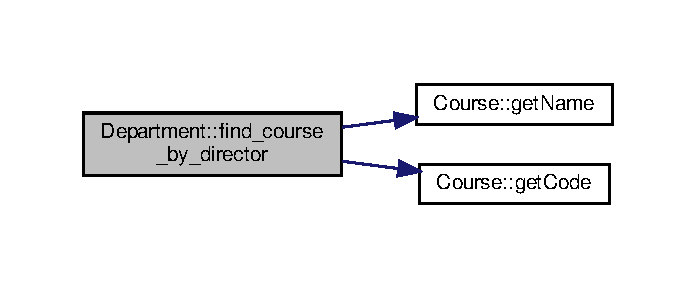
\includegraphics[width=334pt]{classDepartment_a5d83db657bd838d17ac04be757f887a5_cgraph}
\end{center}
\end{figure}
\mbox{\Hypertarget{classDepartment_a2f776e8ddcf895cccdf60beb206b8620}\label{classDepartment_a2f776e8ddcf895cccdf60beb206b8620}} 
\index{Department@{Department}!find\+\_\+course\+\_\+by\+\_\+name@{find\+\_\+course\+\_\+by\+\_\+name}}
\index{find\+\_\+course\+\_\+by\+\_\+name@{find\+\_\+course\+\_\+by\+\_\+name}!Department@{Department}}
\subsubsection{\texorpdfstring{find\+\_\+course\+\_\+by\+\_\+name()}{find\_course\_by\_name()}}
{\footnotesize\ttfamily \hyperlink{classCourse}{Course} $\ast$ Department\+::find\+\_\+course\+\_\+by\+\_\+name (\begin{DoxyParamCaption}\item[{std\+::string}]{name }\end{DoxyParamCaption}) const}

Finds a course by name 
\begin{DoxyParams}{Parameters}
{\em name} & The name of the course to be found \\
\hline
\end{DoxyParams}
\begin{DoxyReturn}{Returns}
The course to be found 
\end{DoxyReturn}


Definition at line 165 of file Department.\+cpp.

Here is the call graph for this function\+:\nopagebreak
\begin{figure}[H]
\begin{center}
\leavevmode
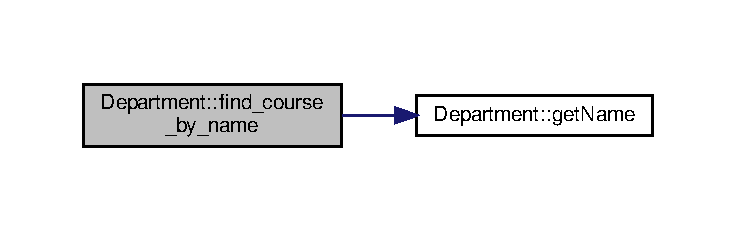
\includegraphics[width=350pt]{classDepartment_a2f776e8ddcf895cccdf60beb206b8620_cgraph}
\end{center}
\end{figure}
\mbox{\Hypertarget{classDepartment_a1a350298618bf4be8cc42eabef377212}\label{classDepartment_a1a350298618bf4be8cc42eabef377212}} 
\index{Department@{Department}!get\+Courses@{get\+Courses}}
\index{get\+Courses@{get\+Courses}!Department@{Department}}
\subsubsection{\texorpdfstring{get\+Courses()}{getCourses()}}
{\footnotesize\ttfamily std\+::vector$<$ \hyperlink{classCourse}{Course} $\ast$ $>$ Department\+::get\+Courses (\begin{DoxyParamCaption}{ }\end{DoxyParamCaption}) const}

Gets the courses of the department. \begin{DoxyReturn}{Returns}
The courses of the department. 
\end{DoxyReturn}


Definition at line 49 of file Department.\+cpp.

\mbox{\Hypertarget{classDepartment_a3ada89e70eae97b429c9a82f601e98c0}\label{classDepartment_a3ada89e70eae97b429c9a82f601e98c0}} 
\index{Department@{Department}!get\+Name@{get\+Name}}
\index{get\+Name@{get\+Name}!Department@{Department}}
\subsubsection{\texorpdfstring{get\+Name()}{getName()}}
{\footnotesize\ttfamily std\+::string Department\+::get\+Name (\begin{DoxyParamCaption}{ }\end{DoxyParamCaption}) const}

Gets the name of the department. \begin{DoxyReturn}{Returns}
The name of the department. 
\end{DoxyReturn}


Definition at line 40 of file Department.\+cpp.

\mbox{\Hypertarget{classDepartment_ab15a7312cdf65f53c3796c428bb6211b}\label{classDepartment_ab15a7312cdf65f53c3796c428bb6211b}} 
\index{Department@{Department}!print\+Info@{print\+Info}}
\index{print\+Info@{print\+Info}!Department@{Department}}
\subsubsection{\texorpdfstring{print\+Info()}{printInfo()}}
{\footnotesize\ttfamily void Department\+::print\+Info (\begin{DoxyParamCaption}{ }\end{DoxyParamCaption}) const}

Prints the information of the department. 

Definition at line 57 of file Department.\+cpp.

Here is the call graph for this function\+:\nopagebreak
\begin{figure}[H]
\begin{center}
\leavevmode
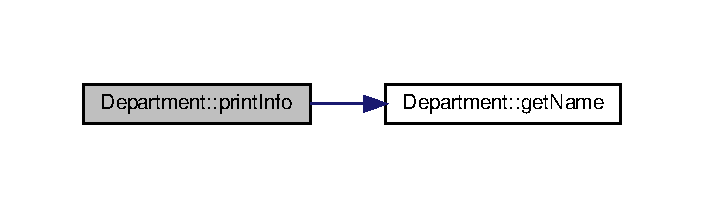
\includegraphics[width=338pt]{classDepartment_ab15a7312cdf65f53c3796c428bb6211b_cgraph}
\end{center}
\end{figure}
\mbox{\Hypertarget{classDepartment_a52742b6ce155016eb084ccd2faccdeef}\label{classDepartment_a52742b6ce155016eb084ccd2faccdeef}} 
\index{Department@{Department}!set\+Courses@{set\+Courses}}
\index{set\+Courses@{set\+Courses}!Department@{Department}}
\subsubsection{\texorpdfstring{set\+Courses()}{setCourses()}}
{\footnotesize\ttfamily void Department\+::set\+Courses (\begin{DoxyParamCaption}\item[{std\+::vector$<$ \hyperlink{classCourse}{Course} $\ast$$>$}]{courses }\end{DoxyParamCaption})}

Sets the courses of the department. 
\begin{DoxyParams}{Parameters}
{\em courses} & The courses of the department. \\
\hline
\end{DoxyParams}


Definition at line 80 of file Department.\+cpp.

\mbox{\Hypertarget{classDepartment_adbde303b8c83a10b3da68ee9f949f731}\label{classDepartment_adbde303b8c83a10b3da68ee9f949f731}} 
\index{Department@{Department}!set\+Name@{set\+Name}}
\index{set\+Name@{set\+Name}!Department@{Department}}
\subsubsection{\texorpdfstring{set\+Name()}{setName()}}
{\footnotesize\ttfamily void Department\+::set\+Name (\begin{DoxyParamCaption}\item[{std\+::string}]{name }\end{DoxyParamCaption})}

Sets the name of the department. 
\begin{DoxyParams}{Parameters}
{\em name} & The name of the department. \\
\hline
\end{DoxyParams}


Definition at line 71 of file Department.\+cpp.

\mbox{\Hypertarget{classDepartment_accf36d58f8b5e8110148f3a69ad30278}\label{classDepartment_accf36d58f8b5e8110148f3a69ad30278}} 
\index{Department@{Department}!sort\+\_\+courses\+\_\+code\+\_\+crescent@{sort\+\_\+courses\+\_\+code\+\_\+crescent}}
\index{sort\+\_\+courses\+\_\+code\+\_\+crescent@{sort\+\_\+courses\+\_\+code\+\_\+crescent}!Department@{Department}}
\subsubsection{\texorpdfstring{sort\+\_\+courses\+\_\+code\+\_\+crescent()}{sort\_courses\_code\_crescent()}}
{\footnotesize\ttfamily void Department\+::sort\+\_\+courses\+\_\+code\+\_\+crescent (\begin{DoxyParamCaption}{ }\end{DoxyParamCaption})}

Sorts courses by code in ascending order 

Definition at line 113 of file Department.\+cpp.

\mbox{\Hypertarget{classDepartment_a320c23411a02eba00f00a15895c538b2}\label{classDepartment_a320c23411a02eba00f00a15895c538b2}} 
\index{Department@{Department}!sort\+\_\+courses\+\_\+code\+\_\+decrescent@{sort\+\_\+courses\+\_\+code\+\_\+decrescent}}
\index{sort\+\_\+courses\+\_\+code\+\_\+decrescent@{sort\+\_\+courses\+\_\+code\+\_\+decrescent}!Department@{Department}}
\subsubsection{\texorpdfstring{sort\+\_\+courses\+\_\+code\+\_\+decrescent()}{sort\_courses\_code\_decrescent()}}
{\footnotesize\ttfamily void Department\+::sort\+\_\+courses\+\_\+code\+\_\+decrescent (\begin{DoxyParamCaption}{ }\end{DoxyParamCaption})}

Sorts courses by code in descending order 

Definition at line 121 of file Department.\+cpp.

\mbox{\Hypertarget{classDepartment_a020f24af6978f0033895e8ebde27bbfb}\label{classDepartment_a020f24af6978f0033895e8ebde27bbfb}} 
\index{Department@{Department}!sort\+\_\+courses\+\_\+name\+\_\+crescent@{sort\+\_\+courses\+\_\+name\+\_\+crescent}}
\index{sort\+\_\+courses\+\_\+name\+\_\+crescent@{sort\+\_\+courses\+\_\+name\+\_\+crescent}!Department@{Department}}
\subsubsection{\texorpdfstring{sort\+\_\+courses\+\_\+name\+\_\+crescent()}{sort\_courses\_name\_crescent()}}
{\footnotesize\ttfamily void Department\+::sort\+\_\+courses\+\_\+name\+\_\+crescent (\begin{DoxyParamCaption}{ }\end{DoxyParamCaption})}

Sorts courses by name in ascending order 

Definition at line 129 of file Department.\+cpp.

\mbox{\Hypertarget{classDepartment_a7798d17dd46c0859cf6ce68c7ec434ae}\label{classDepartment_a7798d17dd46c0859cf6ce68c7ec434ae}} 
\index{Department@{Department}!sort\+\_\+courses\+\_\+name\+\_\+decrescent@{sort\+\_\+courses\+\_\+name\+\_\+decrescent}}
\index{sort\+\_\+courses\+\_\+name\+\_\+decrescent@{sort\+\_\+courses\+\_\+name\+\_\+decrescent}!Department@{Department}}
\subsubsection{\texorpdfstring{sort\+\_\+courses\+\_\+name\+\_\+decrescent()}{sort\_courses\_name\_decrescent()}}
{\footnotesize\ttfamily void Department\+::sort\+\_\+courses\+\_\+name\+\_\+decrescent (\begin{DoxyParamCaption}{ }\end{DoxyParamCaption})}

Sorts courses by name in descending order 

Definition at line 137 of file Department.\+cpp.



The documentation for this class was generated from the following files\+:\begin{DoxyCompactItemize}
\item 
include/Department.\+hpp\item 
src/Department.\+cpp\end{DoxyCompactItemize}

\hypertarget{classFaculty}{}\section{Faculty Class Reference}
\label{classFaculty}\index{Faculty@{Faculty}}
\subsection*{Public Member Functions}
\begin{DoxyCompactItemize}
\item 
\hyperlink{classFaculty_a1c3f6a0eefcd4aee451e8c1db8e658fc}{Faculty} ()
\item 
\hyperlink{classFaculty_ad195c1e251d40e5e324df707e48eca00}{Faculty} (std\+::string name, std\+::vector$<$ \hyperlink{classDepartment}{Department} $\ast$$>$ departments, std\+::vector$<$ \hyperlink{classFacultyMember}{Faculty\+Member} $\ast$$>$ faculty\+Members)
\item 
virtual \hyperlink{classFaculty_ace9ed6a960bd1e1a07a4344ed63bdaf3}{$\sim$\+Faculty} ()
\item 
std\+::vector$<$ \hyperlink{classDepartment}{Department} $\ast$ $>$ \hyperlink{classFaculty_acdf3fba82bf16b6e41fff7d1179d00d5}{get\+Departments} () const
\item 
std\+::string \hyperlink{classFaculty_ad255367a0946117c9161a7214bc0e99d}{get\+Name} () const
\item 
std\+::vector$<$ \hyperlink{classFacultyMember}{Faculty\+Member} $\ast$ $>$ \hyperlink{classFaculty_a92e85922b9fdcef7bce1e9d5018a09e7}{get\+Faculty\+Members} () const
\item 
void \hyperlink{classFaculty_a7c88b74961f730faea3d5c4656580a40}{sort\+\_\+departments\+\_\+name\+\_\+crescent} ()
\item 
void \hyperlink{classFaculty_a8358e69ea6c932ace707bdfc72c399f0}{sort\+\_\+departments\+\_\+name\+\_\+decrescent} ()
\item 
void \hyperlink{classFaculty_a4408cd19b29026bd97bac96a6a026e5b}{sort\+\_\+departments\+\_\+number\+\_\+of\+\_\+courses\+\_\+crescent} ()
\item 
void \hyperlink{classFaculty_a168b261a3fe60485719afb5b1caa1575}{sort\+\_\+departments\+\_\+number\+\_\+of\+\_\+courses\+\_\+decrescent} ()
\item 
void \hyperlink{classFaculty_a1539207b8591b41e32f0108560a7843a}{sort\+\_\+member\+\_\+name\+\_\+crescent} ()
\item 
\mbox{\Hypertarget{classFaculty_aebba7a64ff3c3e0d377b9bd296f07660}\label{classFaculty_aebba7a64ff3c3e0d377b9bd296f07660}} 
void {\bfseries sort\+\_\+member\+\_\+name\+\_\+decrescent} ()
\item 
void \hyperlink{classFaculty_a524f8320d93979695e345f9701c87dd1}{sort\+\_\+member\+\_\+birth\+\_\+date\+\_\+crescent} ()
\item 
void \hyperlink{classFaculty_aa2d7fd660dda947c882c0b02bbdbdc40}{sort\+\_\+member\+\_\+birth\+\_\+date\+\_\+decrescent} ()
\item 
void \hyperlink{classFaculty_abc2a6b1d2ef54e397e47839445d57b03}{sort\+\_\+member\+\_\+code\+\_\+crescent} ()
\item 
void \hyperlink{classFaculty_affc074ff7e6ccca9def97262dc66618e}{sort\+\_\+member\+\_\+code\+\_\+decrescent} ()
\item 
void \hyperlink{classFaculty_acc553daf99e38316f5a0b38cafc2ede8}{add\+Department} (\hyperlink{classDepartment}{Department} $\ast$d)
\item 
void \hyperlink{classFaculty_a0438f29c6c9d9f7ca68fc5193f9639e3}{add\+Faculty\+Member} (\hyperlink{classFacultyMember}{Faculty\+Member} $\ast$fm)
\item 
void \hyperlink{classFaculty_aafc38827c052623298d74669ae908397}{print\+Info} () const
\item 
void \hyperlink{classFaculty_a0059fc30acc3f8d7477cde7a1e32a4d8}{set\+Name} (std\+::string name)
\item 
void \hyperlink{classFaculty_adf74199027a7cfb4d873cb72173b6e5b}{set\+Departments} (std\+::vector$<$ \hyperlink{classDepartment}{Department} $\ast$$>$ departments)
\item 
void \hyperlink{classFaculty_a887b24c4fe91d0c77c055be9473e2d88}{erase\+Department} (\hyperlink{classDepartment}{Department} $\ast$d)
\item 
bool \hyperlink{classFaculty_a780aaae0ddd89dfc175ecdf30b8d3081}{erase\+Faculty\+Member} (\hyperlink{classFacultyMember}{Faculty\+Member} $\ast$fm)
\begin{DoxyCompactList}\small\item\em Erases a faculty member. \end{DoxyCompactList}\item 
\hyperlink{classDepartment}{Department} $\ast$ \hyperlink{classFaculty_adbd64c7f09530fe481586b3d059e237f}{find\+\_\+deparment\+\_\+by\+\_\+name} (std\+::string name) const
\item 
\hyperlink{classFacultyMember}{Faculty\+Member} $\ast$ \hyperlink{classFaculty_ae5b2d7446d9a91bdc1599fee00ee4e6a}{find\+\_\+member\+\_\+by\+\_\+name} (std\+::string name) const
\item 
\hyperlink{classFacultyMember}{Faculty\+Member} $\ast$ \hyperlink{classFaculty_a02524b735865a4eb60ee0c5f681c528f}{find\+\_\+member\+\_\+by\+\_\+code} (int code) const
\item 
vector$<$ \hyperlink{classCourse}{Course} $\ast$ $>$ \hyperlink{classFaculty_a1c959f356e288ee08bb083e669c66742}{get\+Courses} ()
\item 
\hyperlink{classCourse}{Course} $\ast$ \hyperlink{classFaculty_a259de013771e90271b3a58d96a378e12}{find\+Course} (unsigned int code)
\item 
\mbox{\Hypertarget{classFaculty_a9d7afbae98e180224e27a3709e0a3dfb}\label{classFaculty_a9d7afbae98e180224e27a3709e0a3dfb}} 
void {\bfseries add\+Student\+Scholarship\+Queue} (\hyperlink{classStudent}{Student} s)
\item 
\mbox{\Hypertarget{classFaculty_a05ddc9cc00381e30bdd2b2c0d5e9341a}\label{classFaculty_a05ddc9cc00381e30bdd2b2c0d5e9341a}} 
priority\+\_\+queue$<$ \hyperlink{classStudent}{Student} $>$ {\bfseries get\+Scholarship\+Queue} () const
\item 
\mbox{\Hypertarget{classFaculty_a744f766eecf3592724f21f8e6e134122}\label{classFaculty_a744f766eecf3592724f21f8e6e134122}} 
void {\bfseries insert\+Student} (\hyperlink{classStudent}{Student} $\ast$s)
\item 
\mbox{\Hypertarget{classFaculty_a2508e486e3b787c9d3de40b03cc47092}\label{classFaculty_a2508e486e3b787c9d3de40b03cc47092}} 
\hyperlink{classBST}{B\+ST}$<$ \hyperlink{classStudentPtr}{Student\+Ptr} $>$ {\bfseries get\+All\+Students} () const
\item 
\mbox{\Hypertarget{classFaculty_af773eecfbef6d5d364a6c7d0cc5c9f14}\label{classFaculty_af773eecfbef6d5d364a6c7d0cc5c9f14}} 
\hyperlink{classStudent}{Student} $\ast$ {\bfseries find\+Student} (std\+::string name, int course) const
\item 
\mbox{\Hypertarget{classFaculty_a86915acc3b29217b7aebb81f45624e41}\label{classFaculty_a86915acc3b29217b7aebb81f45624e41}} 
void {\bfseries test} ()
\item 
\mbox{\Hypertarget{classFaculty_ab20beb3cbd41b0f75932e4301e2de7af}\label{classFaculty_ab20beb3cbd41b0f75932e4301e2de7af}} 
void {\bfseries add\+Students} (vector$<$ \hyperlink{classStudent}{Student} $\ast$$>$ students\+To\+Add)
\item 
\mbox{\Hypertarget{classFaculty_a59303a88ccd010b8c4cf5b53dc7d2153}\label{classFaculty_a59303a88ccd010b8c4cf5b53dc7d2153}} 
vector$<$ \hyperlink{classStudent}{Student} $\ast$ $>$ {\bfseries get\+Students} () const
\item 
\mbox{\Hypertarget{classFaculty_a3e14c00fa37ab25585a549f3037f0fa9}\label{classFaculty_a3e14c00fa37ab25585a549f3037f0fa9}} 
bool {\bfseries erase\+Student} (\hyperlink{classStudent}{Student} $\ast$s)
\item 
\mbox{\Hypertarget{classFaculty_ad4f56ad6717168df8edcda0175b41827}\label{classFaculty_ad4f56ad6717168df8edcda0175b41827}} 
void {\bfseries compated\+Information} (std\+::ofstream \&f)
\item 
\mbox{\Hypertarget{classFaculty_a3f0c44c19921eeba6677dcefc45e8d20}\label{classFaculty_a3f0c44c19921eeba6677dcefc45e8d20}} 
void {\bfseries set\+Faculty\+Members} (std\+::vector$<$ \hyperlink{classFacultyMember}{Faculty\+Member} $\ast$$>$)
\item 
\mbox{\Hypertarget{classFaculty_adcb450152b935deb3d1a7fecf741b7b8}\label{classFaculty_adcb450152b935deb3d1a7fecf741b7b8}} 
void {\bfseries set\+Students} (std\+::vector$<$ \hyperlink{classStudent}{Student} $\ast$$>$ v)
\item 
\mbox{\Hypertarget{classFaculty_abc4b87bd3404b95815faf1b552c629e9}\label{classFaculty_abc4b87bd3404b95815faf1b552c629e9}} 
void {\bfseries print\+Employee\+Register} ()
\end{DoxyCompactItemize}


\subsection{Detailed Description}


Definition at line 29 of file Faculty.\+hpp.



\subsection{Constructor \& Destructor Documentation}
\mbox{\Hypertarget{classFaculty_a1c3f6a0eefcd4aee451e8c1db8e658fc}\label{classFaculty_a1c3f6a0eefcd4aee451e8c1db8e658fc}} 
\index{Faculty@{Faculty}!Faculty@{Faculty}}
\index{Faculty@{Faculty}!Faculty@{Faculty}}
\subsubsection{\texorpdfstring{Faculty()}{Faculty()}\hspace{0.1cm}{\footnotesize\ttfamily [1/2]}}
{\footnotesize\ttfamily Faculty\+::\+Faculty (\begin{DoxyParamCaption}{ }\end{DoxyParamCaption})}

Constructs a \hyperlink{classFaculty}{Faculty} object. 

Definition at line 7 of file Faculty.\+cpp.

\mbox{\Hypertarget{classFaculty_ad195c1e251d40e5e324df707e48eca00}\label{classFaculty_ad195c1e251d40e5e324df707e48eca00}} 
\index{Faculty@{Faculty}!Faculty@{Faculty}}
\index{Faculty@{Faculty}!Faculty@{Faculty}}
\subsubsection{\texorpdfstring{Faculty()}{Faculty()}\hspace{0.1cm}{\footnotesize\ttfamily [2/2]}}
{\footnotesize\ttfamily Faculty\+::\+Faculty (\begin{DoxyParamCaption}\item[{std\+::string}]{name,  }\item[{std\+::vector$<$ \hyperlink{classDepartment}{Department} $\ast$$>$}]{departments,  }\item[{std\+::vector$<$ \hyperlink{classFacultyMember}{Faculty\+Member} $\ast$$>$}]{faculty\+Members }\end{DoxyParamCaption})}

Constructs a \hyperlink{classFaculty}{Faculty} object with all the attributes as parameters. 
\begin{DoxyParams}{Parameters}
{\em name} & The name of the \hyperlink{classFaculty}{Faculty}. \\
\hline
{\em departments} & The departments of the faculty. \\
\hline
{\em faculty\+Members} & The members of the faculty. \\
\hline
\end{DoxyParams}


Definition at line 15 of file Faculty.\+cpp.

\mbox{\Hypertarget{classFaculty_ace9ed6a960bd1e1a07a4344ed63bdaf3}\label{classFaculty_ace9ed6a960bd1e1a07a4344ed63bdaf3}} 
\index{Faculty@{Faculty}!````~Faculty@{$\sim$\+Faculty}}
\index{````~Faculty@{$\sim$\+Faculty}!Faculty@{Faculty}}
\subsubsection{\texorpdfstring{$\sim$\+Faculty()}{~Faculty()}}
{\footnotesize\ttfamily Faculty\+::$\sim$\+Faculty (\begin{DoxyParamCaption}{ }\end{DoxyParamCaption})\hspace{0.3cm}{\ttfamily [virtual]}}

Destroys a \hyperlink{classFaculty}{Faculty} object by deleting object in the vectors departments and faculty\+Members. 

Definition at line 31 of file Faculty.\+cpp.



\subsection{Member Function Documentation}
\mbox{\Hypertarget{classFaculty_acc553daf99e38316f5a0b38cafc2ede8}\label{classFaculty_acc553daf99e38316f5a0b38cafc2ede8}} 
\index{Faculty@{Faculty}!add\+Department@{add\+Department}}
\index{add\+Department@{add\+Department}!Faculty@{Faculty}}
\subsubsection{\texorpdfstring{add\+Department()}{addDepartment()}}
{\footnotesize\ttfamily void Faculty\+::add\+Department (\begin{DoxyParamCaption}\item[{\hyperlink{classDepartment}{Department} $\ast$}]{d }\end{DoxyParamCaption})}

Adds a department to the faculty. 
\begin{DoxyParams}{Parameters}
{\em d} & A department. \\
\hline
\end{DoxyParams}


Definition at line 282 of file Faculty.\+cpp.

\mbox{\Hypertarget{classFaculty_a0438f29c6c9d9f7ca68fc5193f9639e3}\label{classFaculty_a0438f29c6c9d9f7ca68fc5193f9639e3}} 
\index{Faculty@{Faculty}!add\+Faculty\+Member@{add\+Faculty\+Member}}
\index{add\+Faculty\+Member@{add\+Faculty\+Member}!Faculty@{Faculty}}
\subsubsection{\texorpdfstring{add\+Faculty\+Member()}{addFacultyMember()}}
{\footnotesize\ttfamily void Faculty\+::add\+Faculty\+Member (\begin{DoxyParamCaption}\item[{\hyperlink{classFacultyMember}{Faculty\+Member} $\ast$}]{fm }\end{DoxyParamCaption})}

Adds a faculty member to the university. 
\begin{DoxyParams}{Parameters}
{\em fm} & A faculty member. \\
\hline
\end{DoxyParams}


Definition at line 309 of file Faculty.\+cpp.

\mbox{\Hypertarget{classFaculty_a887b24c4fe91d0c77c055be9473e2d88}\label{classFaculty_a887b24c4fe91d0c77c055be9473e2d88}} 
\index{Faculty@{Faculty}!erase\+Department@{erase\+Department}}
\index{erase\+Department@{erase\+Department}!Faculty@{Faculty}}
\subsubsection{\texorpdfstring{erase\+Department()}{eraseDepartment()}}
{\footnotesize\ttfamily void Faculty\+::erase\+Department (\begin{DoxyParamCaption}\item[{\hyperlink{classDepartment}{Department} $\ast$}]{d }\end{DoxyParamCaption})}

Erases a department of the faculty. 
\begin{DoxyParams}{Parameters}
{\em d} & A department of the faculty. \\
\hline
\end{DoxyParams}


Definition at line 349 of file Faculty.\+cpp.

\mbox{\Hypertarget{classFaculty_a780aaae0ddd89dfc175ecdf30b8d3081}\label{classFaculty_a780aaae0ddd89dfc175ecdf30b8d3081}} 
\index{Faculty@{Faculty}!erase\+Faculty\+Member@{erase\+Faculty\+Member}}
\index{erase\+Faculty\+Member@{erase\+Faculty\+Member}!Faculty@{Faculty}}
\subsubsection{\texorpdfstring{erase\+Faculty\+Member()}{eraseFacultyMember()}}
{\footnotesize\ttfamily bool Faculty\+::erase\+Faculty\+Member (\begin{DoxyParamCaption}\item[{\hyperlink{classFacultyMember}{Faculty\+Member} $\ast$}]{fm }\end{DoxyParamCaption})}



Erases a faculty member. 


\begin{DoxyParams}{Parameters}
{\em fm} & A faculty member \\
\hline
\end{DoxyParams}
\begin{DoxyReturn}{Returns}
true Found the member and deleted it 

false Didn\textquotesingle{}t find the member and, thus, didn\textquotesingle{}t delete it 
\end{DoxyReturn}


Definition at line 368 of file Faculty.\+cpp.

\mbox{\Hypertarget{classFaculty_adbd64c7f09530fe481586b3d059e237f}\label{classFaculty_adbd64c7f09530fe481586b3d059e237f}} 
\index{Faculty@{Faculty}!find\+\_\+deparment\+\_\+by\+\_\+name@{find\+\_\+deparment\+\_\+by\+\_\+name}}
\index{find\+\_\+deparment\+\_\+by\+\_\+name@{find\+\_\+deparment\+\_\+by\+\_\+name}!Faculty@{Faculty}}
\subsubsection{\texorpdfstring{find\+\_\+deparment\+\_\+by\+\_\+name()}{find\_deparment\_by\_name()}}
{\footnotesize\ttfamily \hyperlink{classDepartment}{Department} $\ast$ Faculty\+::find\+\_\+deparment\+\_\+by\+\_\+name (\begin{DoxyParamCaption}\item[{std\+::string}]{name }\end{DoxyParamCaption}) const}

Finds a department with the provided name 
\begin{DoxyParams}{Parameters}
{\em name} & The name of the department to find \\
\hline
\end{DoxyParams}
\begin{DoxyReturn}{Returns}
A pointer to the found department, or, if not found, a N\+U\+LL pointer 
\end{DoxyReturn}


Definition at line 400 of file Faculty.\+cpp.

Here is the call graph for this function\+:\nopagebreak
\begin{figure}[H]
\begin{center}
\leavevmode
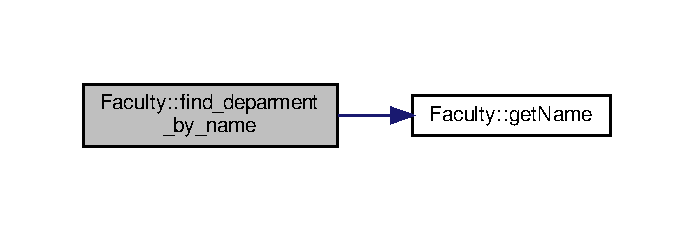
\includegraphics[width=333pt]{classFaculty_adbd64c7f09530fe481586b3d059e237f_cgraph}
\end{center}
\end{figure}
\mbox{\Hypertarget{classFaculty_a02524b735865a4eb60ee0c5f681c528f}\label{classFaculty_a02524b735865a4eb60ee0c5f681c528f}} 
\index{Faculty@{Faculty}!find\+\_\+member\+\_\+by\+\_\+code@{find\+\_\+member\+\_\+by\+\_\+code}}
\index{find\+\_\+member\+\_\+by\+\_\+code@{find\+\_\+member\+\_\+by\+\_\+code}!Faculty@{Faculty}}
\subsubsection{\texorpdfstring{find\+\_\+member\+\_\+by\+\_\+code()}{find\_member\_by\_code()}}
{\footnotesize\ttfamily \hyperlink{classFacultyMember}{Faculty\+Member} $\ast$ Faculty\+::find\+\_\+member\+\_\+by\+\_\+code (\begin{DoxyParamCaption}\item[{int}]{code }\end{DoxyParamCaption}) const}

Finds a faculty member with the provided name 
\begin{DoxyParams}{Parameters}
{\em code} & The code of faculty member \\
\hline
\end{DoxyParams}
\begin{DoxyReturn}{Returns}
A pointer to the found department, or, if not found, a N\+U\+LL pointer 
\end{DoxyReturn}


Definition at line 438 of file Faculty.\+cpp.

\mbox{\Hypertarget{classFaculty_ae5b2d7446d9a91bdc1599fee00ee4e6a}\label{classFaculty_ae5b2d7446d9a91bdc1599fee00ee4e6a}} 
\index{Faculty@{Faculty}!find\+\_\+member\+\_\+by\+\_\+name@{find\+\_\+member\+\_\+by\+\_\+name}}
\index{find\+\_\+member\+\_\+by\+\_\+name@{find\+\_\+member\+\_\+by\+\_\+name}!Faculty@{Faculty}}
\subsubsection{\texorpdfstring{find\+\_\+member\+\_\+by\+\_\+name()}{find\_member\_by\_name()}}
{\footnotesize\ttfamily \hyperlink{classFacultyMember}{Faculty\+Member} $\ast$ Faculty\+::find\+\_\+member\+\_\+by\+\_\+name (\begin{DoxyParamCaption}\item[{std\+::string}]{name }\end{DoxyParamCaption}) const}

Finds a faculty member with the provided name 
\begin{DoxyParams}{Parameters}
{\em name} & The name of faculty member \\
\hline
\end{DoxyParams}
\begin{DoxyReturn}{Returns}
A pointer to the found department, or, if not found, a N\+U\+LL pointer 
\end{DoxyReturn}


Definition at line 419 of file Faculty.\+cpp.

Here is the call graph for this function\+:\nopagebreak
\begin{figure}[H]
\begin{center}
\leavevmode
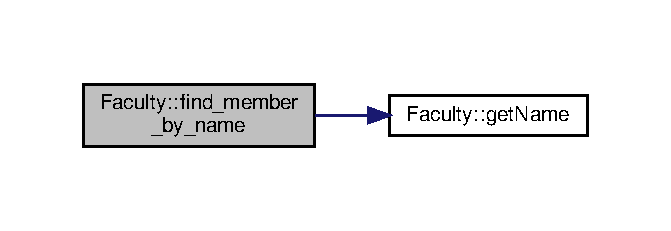
\includegraphics[width=322pt]{classFaculty_ae5b2d7446d9a91bdc1599fee00ee4e6a_cgraph}
\end{center}
\end{figure}
\mbox{\Hypertarget{classFaculty_a259de013771e90271b3a58d96a378e12}\label{classFaculty_a259de013771e90271b3a58d96a378e12}} 
\index{Faculty@{Faculty}!find\+Course@{find\+Course}}
\index{find\+Course@{find\+Course}!Faculty@{Faculty}}
\subsubsection{\texorpdfstring{find\+Course()}{findCourse()}}
{\footnotesize\ttfamily \hyperlink{classCourse}{Course} $\ast$ Faculty\+::find\+Course (\begin{DoxyParamCaption}\item[{unsigned int}]{code }\end{DoxyParamCaption})}

Finds the course of the faculty. 
\begin{DoxyParams}{Parameters}
{\em code} & The code of a course. \\
\hline
\end{DoxyParams}
\begin{DoxyReturn}{Returns}
A pointer to a course. 
\end{DoxyReturn}


Definition at line 473 of file Faculty.\+cpp.

Here is the call graph for this function\+:\nopagebreak
\begin{figure}[H]
\begin{center}
\leavevmode
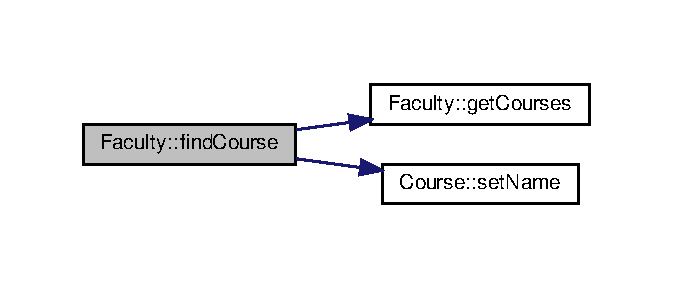
\includegraphics[width=323pt]{classFaculty_a259de013771e90271b3a58d96a378e12_cgraph}
\end{center}
\end{figure}
\mbox{\Hypertarget{classFaculty_a1c959f356e288ee08bb083e669c66742}\label{classFaculty_a1c959f356e288ee08bb083e669c66742}} 
\index{Faculty@{Faculty}!get\+Courses@{get\+Courses}}
\index{get\+Courses@{get\+Courses}!Faculty@{Faculty}}
\subsubsection{\texorpdfstring{get\+Courses()}{getCourses()}}
{\footnotesize\ttfamily vector$<$ \hyperlink{classCourse}{Course} $\ast$ $>$ Faculty\+::get\+Courses (\begin{DoxyParamCaption}{ }\end{DoxyParamCaption})}

Gets every course of the faculty. \begin{DoxyReturn}{Returns}
Every course of the faculty. 
\end{DoxyReturn}


Definition at line 455 of file Faculty.\+cpp.

\mbox{\Hypertarget{classFaculty_acdf3fba82bf16b6e41fff7d1179d00d5}\label{classFaculty_acdf3fba82bf16b6e41fff7d1179d00d5}} 
\index{Faculty@{Faculty}!get\+Departments@{get\+Departments}}
\index{get\+Departments@{get\+Departments}!Faculty@{Faculty}}
\subsubsection{\texorpdfstring{get\+Departments()}{getDepartments()}}
{\footnotesize\ttfamily std\+::vector$<$ \hyperlink{classDepartment}{Department} $\ast$ $>$ Faculty\+::get\+Departments (\begin{DoxyParamCaption}{ }\end{DoxyParamCaption}) const}

Gets the departments of the \hyperlink{classFaculty}{Faculty}. \begin{DoxyReturn}{Returns}
The departments of the faculty. 
\end{DoxyReturn}


Definition at line 51 of file Faculty.\+cpp.

\mbox{\Hypertarget{classFaculty_a92e85922b9fdcef7bce1e9d5018a09e7}\label{classFaculty_a92e85922b9fdcef7bce1e9d5018a09e7}} 
\index{Faculty@{Faculty}!get\+Faculty\+Members@{get\+Faculty\+Members}}
\index{get\+Faculty\+Members@{get\+Faculty\+Members}!Faculty@{Faculty}}
\subsubsection{\texorpdfstring{get\+Faculty\+Members()}{getFacultyMembers()}}
{\footnotesize\ttfamily std\+::vector$<$ \hyperlink{classFacultyMember}{Faculty\+Member} $\ast$ $>$ Faculty\+::get\+Faculty\+Members (\begin{DoxyParamCaption}{ }\end{DoxyParamCaption}) const}

Gets the members of the faculty. \begin{DoxyReturn}{Returns}
The members of the faculty. 
\end{DoxyReturn}


Definition at line 69 of file Faculty.\+cpp.

\mbox{\Hypertarget{classFaculty_ad255367a0946117c9161a7214bc0e99d}\label{classFaculty_ad255367a0946117c9161a7214bc0e99d}} 
\index{Faculty@{Faculty}!get\+Name@{get\+Name}}
\index{get\+Name@{get\+Name}!Faculty@{Faculty}}
\subsubsection{\texorpdfstring{get\+Name()}{getName()}}
{\footnotesize\ttfamily std\+::string Faculty\+::get\+Name (\begin{DoxyParamCaption}{ }\end{DoxyParamCaption}) const}

Gets the name of the \hyperlink{classFaculty}{Faculty}. \begin{DoxyReturn}{Returns}
The name of the faculty. 
\end{DoxyReturn}


Definition at line 60 of file Faculty.\+cpp.

\mbox{\Hypertarget{classFaculty_aafc38827c052623298d74669ae908397}\label{classFaculty_aafc38827c052623298d74669ae908397}} 
\index{Faculty@{Faculty}!print\+Info@{print\+Info}}
\index{print\+Info@{print\+Info}!Faculty@{Faculty}}
\subsubsection{\texorpdfstring{print\+Info()}{printInfo()}}
{\footnotesize\ttfamily void Faculty\+::print\+Info (\begin{DoxyParamCaption}{ }\end{DoxyParamCaption}) const}

Prints the information of a faculty, which is all the values of its attributes. 

Definition at line 291 of file Faculty.\+cpp.

Here is the call graph for this function\+:\nopagebreak
\begin{figure}[H]
\begin{center}
\leavevmode
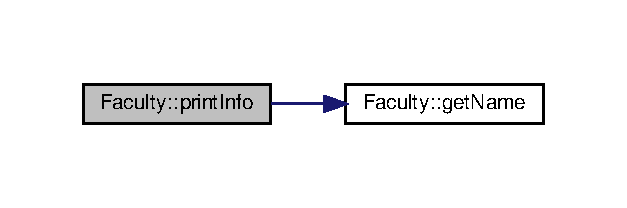
\includegraphics[width=301pt]{classFaculty_aafc38827c052623298d74669ae908397_cgraph}
\end{center}
\end{figure}
\mbox{\Hypertarget{classFaculty_adf74199027a7cfb4d873cb72173b6e5b}\label{classFaculty_adf74199027a7cfb4d873cb72173b6e5b}} 
\index{Faculty@{Faculty}!set\+Departments@{set\+Departments}}
\index{set\+Departments@{set\+Departments}!Faculty@{Faculty}}
\subsubsection{\texorpdfstring{set\+Departments()}{setDepartments()}}
{\footnotesize\ttfamily void Faculty\+::set\+Departments (\begin{DoxyParamCaption}\item[{std\+::vector$<$ \hyperlink{classDepartment}{Department} $\ast$$>$}]{departments }\end{DoxyParamCaption})}

Sets the departments of the faculty. 
\begin{DoxyParams}{Parameters}
{\em departments} & Some departments for the faculty. \\
\hline
\end{DoxyParams}


Definition at line 340 of file Faculty.\+cpp.

\mbox{\Hypertarget{classFaculty_a0059fc30acc3f8d7477cde7a1e32a4d8}\label{classFaculty_a0059fc30acc3f8d7477cde7a1e32a4d8}} 
\index{Faculty@{Faculty}!set\+Name@{set\+Name}}
\index{set\+Name@{set\+Name}!Faculty@{Faculty}}
\subsubsection{\texorpdfstring{set\+Name()}{setName()}}
{\footnotesize\ttfamily void Faculty\+::set\+Name (\begin{DoxyParamCaption}\item[{std\+::string}]{name }\end{DoxyParamCaption})}

Sets the name of the faculty. 
\begin{DoxyParams}{Parameters}
{\em name} & A name for the faculty. \\
\hline
\end{DoxyParams}


Definition at line 331 of file Faculty.\+cpp.

\mbox{\Hypertarget{classFaculty_a7c88b74961f730faea3d5c4656580a40}\label{classFaculty_a7c88b74961f730faea3d5c4656580a40}} 
\index{Faculty@{Faculty}!sort\+\_\+departments\+\_\+name\+\_\+crescent@{sort\+\_\+departments\+\_\+name\+\_\+crescent}}
\index{sort\+\_\+departments\+\_\+name\+\_\+crescent@{sort\+\_\+departments\+\_\+name\+\_\+crescent}!Faculty@{Faculty}}
\subsubsection{\texorpdfstring{sort\+\_\+departments\+\_\+name\+\_\+crescent()}{sort\_departments\_name\_crescent()}}
{\footnotesize\ttfamily void Faculty\+::sort\+\_\+departments\+\_\+name\+\_\+crescent (\begin{DoxyParamCaption}{ }\end{DoxyParamCaption})}

Sorts the departments by name in ascending order 

Definition at line 77 of file Faculty.\+cpp.

\mbox{\Hypertarget{classFaculty_a8358e69ea6c932ace707bdfc72c399f0}\label{classFaculty_a8358e69ea6c932ace707bdfc72c399f0}} 
\index{Faculty@{Faculty}!sort\+\_\+departments\+\_\+name\+\_\+decrescent@{sort\+\_\+departments\+\_\+name\+\_\+decrescent}}
\index{sort\+\_\+departments\+\_\+name\+\_\+decrescent@{sort\+\_\+departments\+\_\+name\+\_\+decrescent}!Faculty@{Faculty}}
\subsubsection{\texorpdfstring{sort\+\_\+departments\+\_\+name\+\_\+decrescent()}{sort\_departments\_name\_decrescent()}}
{\footnotesize\ttfamily void Faculty\+::sort\+\_\+departments\+\_\+name\+\_\+decrescent (\begin{DoxyParamCaption}{ }\end{DoxyParamCaption})}

Sorts the departments by name in descending order 

Definition at line 85 of file Faculty.\+cpp.

\mbox{\Hypertarget{classFaculty_a4408cd19b29026bd97bac96a6a026e5b}\label{classFaculty_a4408cd19b29026bd97bac96a6a026e5b}} 
\index{Faculty@{Faculty}!sort\+\_\+departments\+\_\+number\+\_\+of\+\_\+courses\+\_\+crescent@{sort\+\_\+departments\+\_\+number\+\_\+of\+\_\+courses\+\_\+crescent}}
\index{sort\+\_\+departments\+\_\+number\+\_\+of\+\_\+courses\+\_\+crescent@{sort\+\_\+departments\+\_\+number\+\_\+of\+\_\+courses\+\_\+crescent}!Faculty@{Faculty}}
\subsubsection{\texorpdfstring{sort\+\_\+departments\+\_\+number\+\_\+of\+\_\+courses\+\_\+crescent()}{sort\_departments\_number\_of\_courses\_crescent()}}
{\footnotesize\ttfamily void Faculty\+::sort\+\_\+departments\+\_\+number\+\_\+of\+\_\+courses\+\_\+crescent (\begin{DoxyParamCaption}{ }\end{DoxyParamCaption})}

Sorts departments by number of courses in ascending order 

Definition at line 93 of file Faculty.\+cpp.

\mbox{\Hypertarget{classFaculty_a168b261a3fe60485719afb5b1caa1575}\label{classFaculty_a168b261a3fe60485719afb5b1caa1575}} 
\index{Faculty@{Faculty}!sort\+\_\+departments\+\_\+number\+\_\+of\+\_\+courses\+\_\+decrescent@{sort\+\_\+departments\+\_\+number\+\_\+of\+\_\+courses\+\_\+decrescent}}
\index{sort\+\_\+departments\+\_\+number\+\_\+of\+\_\+courses\+\_\+decrescent@{sort\+\_\+departments\+\_\+number\+\_\+of\+\_\+courses\+\_\+decrescent}!Faculty@{Faculty}}
\subsubsection{\texorpdfstring{sort\+\_\+departments\+\_\+number\+\_\+of\+\_\+courses\+\_\+decrescent()}{sort\_departments\_number\_of\_courses\_decrescent()}}
{\footnotesize\ttfamily void Faculty\+::sort\+\_\+departments\+\_\+number\+\_\+of\+\_\+courses\+\_\+decrescent (\begin{DoxyParamCaption}{ }\end{DoxyParamCaption})}

Sorts departments by number of courses in descending order 

Definition at line 101 of file Faculty.\+cpp.

\mbox{\Hypertarget{classFaculty_a524f8320d93979695e345f9701c87dd1}\label{classFaculty_a524f8320d93979695e345f9701c87dd1}} 
\index{Faculty@{Faculty}!sort\+\_\+member\+\_\+birth\+\_\+date\+\_\+crescent@{sort\+\_\+member\+\_\+birth\+\_\+date\+\_\+crescent}}
\index{sort\+\_\+member\+\_\+birth\+\_\+date\+\_\+crescent@{sort\+\_\+member\+\_\+birth\+\_\+date\+\_\+crescent}!Faculty@{Faculty}}
\subsubsection{\texorpdfstring{sort\+\_\+member\+\_\+birth\+\_\+date\+\_\+crescent()}{sort\_member\_birth\_date\_crescent()}}
{\footnotesize\ttfamily void Faculty\+::sort\+\_\+member\+\_\+birth\+\_\+date\+\_\+crescent (\begin{DoxyParamCaption}{ }\end{DoxyParamCaption})}

Sorts members by birth date in ascending order 

Definition at line 117 of file Faculty.\+cpp.

\mbox{\Hypertarget{classFaculty_aa2d7fd660dda947c882c0b02bbdbdc40}\label{classFaculty_aa2d7fd660dda947c882c0b02bbdbdc40}} 
\index{Faculty@{Faculty}!sort\+\_\+member\+\_\+birth\+\_\+date\+\_\+decrescent@{sort\+\_\+member\+\_\+birth\+\_\+date\+\_\+decrescent}}
\index{sort\+\_\+member\+\_\+birth\+\_\+date\+\_\+decrescent@{sort\+\_\+member\+\_\+birth\+\_\+date\+\_\+decrescent}!Faculty@{Faculty}}
\subsubsection{\texorpdfstring{sort\+\_\+member\+\_\+birth\+\_\+date\+\_\+decrescent()}{sort\_member\_birth\_date\_decrescent()}}
{\footnotesize\ttfamily void Faculty\+::sort\+\_\+member\+\_\+birth\+\_\+date\+\_\+decrescent (\begin{DoxyParamCaption}{ }\end{DoxyParamCaption})}

Sorts members by birth date in descending order 

Definition at line 125 of file Faculty.\+cpp.

\mbox{\Hypertarget{classFaculty_abc2a6b1d2ef54e397e47839445d57b03}\label{classFaculty_abc2a6b1d2ef54e397e47839445d57b03}} 
\index{Faculty@{Faculty}!sort\+\_\+member\+\_\+code\+\_\+crescent@{sort\+\_\+member\+\_\+code\+\_\+crescent}}
\index{sort\+\_\+member\+\_\+code\+\_\+crescent@{sort\+\_\+member\+\_\+code\+\_\+crescent}!Faculty@{Faculty}}
\subsubsection{\texorpdfstring{sort\+\_\+member\+\_\+code\+\_\+crescent()}{sort\_member\_code\_crescent()}}
{\footnotesize\ttfamily void Faculty\+::sort\+\_\+member\+\_\+code\+\_\+crescent (\begin{DoxyParamCaption}{ }\end{DoxyParamCaption})}

Sorts members by code in ascending order 

Definition at line 133 of file Faculty.\+cpp.

\mbox{\Hypertarget{classFaculty_affc074ff7e6ccca9def97262dc66618e}\label{classFaculty_affc074ff7e6ccca9def97262dc66618e}} 
\index{Faculty@{Faculty}!sort\+\_\+member\+\_\+code\+\_\+decrescent@{sort\+\_\+member\+\_\+code\+\_\+decrescent}}
\index{sort\+\_\+member\+\_\+code\+\_\+decrescent@{sort\+\_\+member\+\_\+code\+\_\+decrescent}!Faculty@{Faculty}}
\subsubsection{\texorpdfstring{sort\+\_\+member\+\_\+code\+\_\+decrescent()}{sort\_member\_code\_decrescent()}}
{\footnotesize\ttfamily void Faculty\+::sort\+\_\+member\+\_\+code\+\_\+decrescent (\begin{DoxyParamCaption}{ }\end{DoxyParamCaption})}

Sorts members by code in descending order 

Definition at line 141 of file Faculty.\+cpp.

Here is the call graph for this function\+:\nopagebreak
\begin{figure}[H]
\begin{center}
\leavevmode
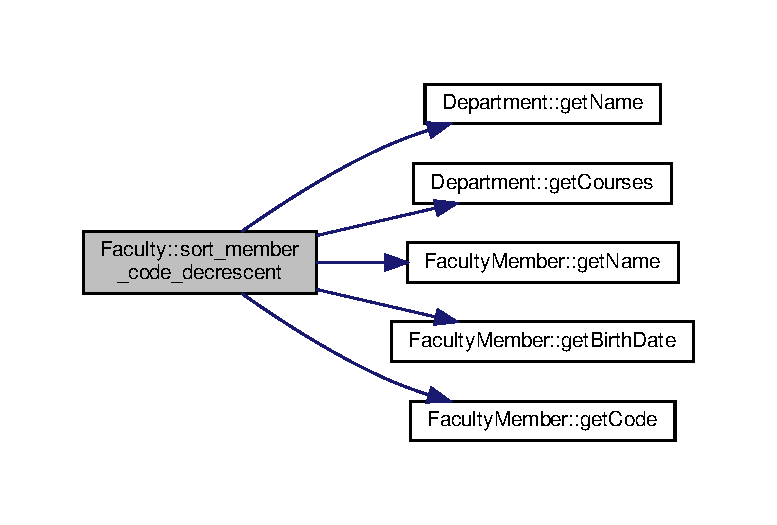
\includegraphics[width=350pt]{classFaculty_affc074ff7e6ccca9def97262dc66618e_cgraph}
\end{center}
\end{figure}
\mbox{\Hypertarget{classFaculty_a1539207b8591b41e32f0108560a7843a}\label{classFaculty_a1539207b8591b41e32f0108560a7843a}} 
\index{Faculty@{Faculty}!sort\+\_\+member\+\_\+name\+\_\+crescent@{sort\+\_\+member\+\_\+name\+\_\+crescent}}
\index{sort\+\_\+member\+\_\+name\+\_\+crescent@{sort\+\_\+member\+\_\+name\+\_\+crescent}!Faculty@{Faculty}}
\subsubsection{\texorpdfstring{sort\+\_\+member\+\_\+name\+\_\+crescent()}{sort\_member\_name\_crescent()}}
{\footnotesize\ttfamily void Faculty\+::sort\+\_\+member\+\_\+name\+\_\+crescent (\begin{DoxyParamCaption}{ }\end{DoxyParamCaption})}

Sorts members by name in ascending order 

Definition at line 109 of file Faculty.\+cpp.



The documentation for this class was generated from the following files\+:\begin{DoxyCompactItemize}
\item 
include/Faculty.\+hpp\item 
src/Faculty.\+cpp\end{DoxyCompactItemize}

\hypertarget{classFacultyMember}{}\section{Faculty\+Member Class Reference}
\label{classFacultyMember}\index{Faculty\+Member@{Faculty\+Member}}


Inheritance diagram for Faculty\+Member\+:\nopagebreak
\begin{figure}[H]
\begin{center}
\leavevmode
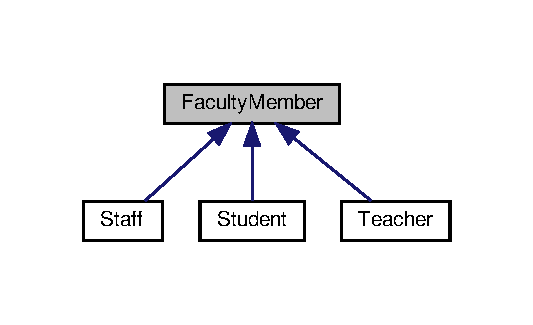
\includegraphics[width=256pt]{classFacultyMember__inherit__graph}
\end{center}
\end{figure}


Collaboration diagram for Faculty\+Member\+:\nopagebreak
\begin{figure}[H]
\begin{center}
\leavevmode
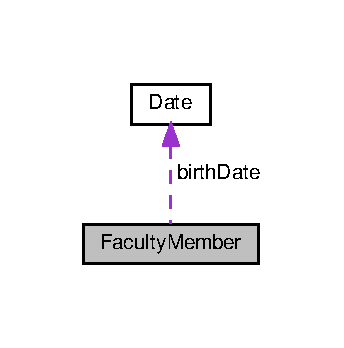
\includegraphics[width=165pt]{classFacultyMember__coll__graph}
\end{center}
\end{figure}
\subsection*{Public Member Functions}
\begin{DoxyCompactItemize}
\item 
\hyperlink{classFacultyMember_a02d3bfb88e071e17053309606544ca29}{Faculty\+Member} (std\+::string name, std\+::string address, \hyperlink{classDate}{Date} birth\+Date, int cellphone\+Number, int code)
\item 
std\+::string \hyperlink{classFacultyMember_a31db85e875c2cfaa8a23d46ab24cf3d6}{get\+Name} () const
\item 
std\+::string \hyperlink{classFacultyMember_a014ef6fda0eedf6644a46504958790f9}{get\+Address} () const
\item 
\hyperlink{classDate}{Date} \hyperlink{classFacultyMember_add1edcb7b45d0061dea8c8ba06cfe7b4}{get\+Birth\+Date} () const
\item 
int \hyperlink{classFacultyMember_a865d91cdeec9e344021da0cf6c9fc29e}{get\+Cellphone\+Number} () const
\item 
int \hyperlink{classFacultyMember_a475a9855e4587df3022c997732ef43b4}{get\+Code} () const
\item 
virtual void \hyperlink{classFacultyMember_af07c814d58d1a2e309c74a0c57b95fd1}{print\+Info} () const
\item 
void \hyperlink{classFacultyMember_a7e4ef8e1a740e7e46d17ed9df43bc5d8}{set\+Name} (std\+::string name)
\item 
void \hyperlink{classFacultyMember_a25dc17f307ac885a7b3722a7685cb517}{set\+Address} (std\+::string address)
\item 
void \hyperlink{classFacultyMember_abec27c8af8bd8274a3ea560da0f12cbd}{set\+Date} (\hyperlink{classDate}{Date} date)
\item 
void \hyperlink{classFacultyMember_aceb0270b28a96e52cfe138c26f3936a4}{set\+Cellphone\+Number} (int cellphone\+Number)
\item 
void \hyperlink{classFacultyMember_acb54ae36938fc1b96bdb1ae8060c29c1}{set\+Code} (int code)
\item 
\mbox{\Hypertarget{classFacultyMember_a263ea4bc1cb7eb281a2fb6f5d1581fda}\label{classFacultyMember_a263ea4bc1cb7eb281a2fb6f5d1581fda}} 
void {\bfseries set\+Birth\+Date} (std\+::string date)
\item 
\mbox{\Hypertarget{classFacultyMember_ab5722a59419ab94768c82d0749c1b687}\label{classFacultyMember_ab5722a59419ab94768c82d0749c1b687}} 
virtual void {\bfseries compated\+Information} (std\+::ofstream \&f)
\end{DoxyCompactItemize}
\subsection*{Protected Attributes}
\begin{DoxyCompactItemize}
\item 
\mbox{\Hypertarget{classFacultyMember_a1db0d896f97f2ef4e38aa84bf6720f9e}\label{classFacultyMember_a1db0d896f97f2ef4e38aa84bf6720f9e}} 
std\+::string {\bfseries name}
\item 
\mbox{\Hypertarget{classFacultyMember_adaecb566a4413d65f3ff4b9ba0048fc7}\label{classFacultyMember_adaecb566a4413d65f3ff4b9ba0048fc7}} 
std\+::string {\bfseries address}
\item 
\mbox{\Hypertarget{classFacultyMember_ac859efad6315ad7a295728d8db4d85f3}\label{classFacultyMember_ac859efad6315ad7a295728d8db4d85f3}} 
\hyperlink{classDate}{Date} {\bfseries birth\+Date}
\item 
\mbox{\Hypertarget{classFacultyMember_a599fa2364bdb3e9365c3cf2f678f028a}\label{classFacultyMember_a599fa2364bdb3e9365c3cf2f678f028a}} 
int {\bfseries cellphone\+Number}
\item 
\mbox{\Hypertarget{classFacultyMember_a925536a617e1222236daf8e96864b1f2}\label{classFacultyMember_a925536a617e1222236daf8e96864b1f2}} 
int {\bfseries code}
\end{DoxyCompactItemize}


\subsection{Detailed Description}


Definition at line 12 of file Faculty\+Member.\+hpp.



\subsection{Constructor \& Destructor Documentation}
\mbox{\Hypertarget{classFacultyMember_a02d3bfb88e071e17053309606544ca29}\label{classFacultyMember_a02d3bfb88e071e17053309606544ca29}} 
\index{Faculty\+Member@{Faculty\+Member}!Faculty\+Member@{Faculty\+Member}}
\index{Faculty\+Member@{Faculty\+Member}!Faculty\+Member@{Faculty\+Member}}
\subsubsection{\texorpdfstring{Faculty\+Member()}{FacultyMember()}}
{\footnotesize\ttfamily Faculty\+Member\+::\+Faculty\+Member (\begin{DoxyParamCaption}\item[{std\+::string}]{name,  }\item[{std\+::string}]{address,  }\item[{\hyperlink{classDate}{Date}}]{birth\+Date,  }\item[{int}]{cellphone\+Number,  }\item[{int}]{code }\end{DoxyParamCaption})}

Constructs a \hyperlink{classFacultyMember}{Faculty\+Member} object. 
\begin{DoxyParams}{Parameters}
{\em name} & The name of a faculty member. \\
\hline
{\em address} & The address of a faculty member. \\
\hline
{\em birth\+Date} & The birth date of a faculty member. \\
\hline
{\em cellphone\+Number} & The cellphone number of a faculty member. \\
\hline
{\em code} & The code of a faculty member. \\
\hline
\end{DoxyParams}


Definition at line 11 of file Faculty\+Member.\+cpp.



\subsection{Member Function Documentation}
\mbox{\Hypertarget{classFacultyMember_a014ef6fda0eedf6644a46504958790f9}\label{classFacultyMember_a014ef6fda0eedf6644a46504958790f9}} 
\index{Faculty\+Member@{Faculty\+Member}!get\+Address@{get\+Address}}
\index{get\+Address@{get\+Address}!Faculty\+Member@{Faculty\+Member}}
\subsubsection{\texorpdfstring{get\+Address()}{getAddress()}}
{\footnotesize\ttfamily std\+::string Faculty\+Member\+::get\+Address (\begin{DoxyParamCaption}{ }\end{DoxyParamCaption}) const}

Gets the address of a faculty member. \begin{DoxyReturn}{Returns}
The address of a faculty member. 
\end{DoxyReturn}


Definition at line 52 of file Faculty\+Member.\+cpp.

\mbox{\Hypertarget{classFacultyMember_add1edcb7b45d0061dea8c8ba06cfe7b4}\label{classFacultyMember_add1edcb7b45d0061dea8c8ba06cfe7b4}} 
\index{Faculty\+Member@{Faculty\+Member}!get\+Birth\+Date@{get\+Birth\+Date}}
\index{get\+Birth\+Date@{get\+Birth\+Date}!Faculty\+Member@{Faculty\+Member}}
\subsubsection{\texorpdfstring{get\+Birth\+Date()}{getBirthDate()}}
{\footnotesize\ttfamily \hyperlink{classDate}{Date} Faculty\+Member\+::get\+Birth\+Date (\begin{DoxyParamCaption}{ }\end{DoxyParamCaption}) const}

Gets the birth date of a faculty member. \begin{DoxyReturn}{Returns}
The birth date of a faculty member. 
\end{DoxyReturn}


Definition at line 61 of file Faculty\+Member.\+cpp.

\mbox{\Hypertarget{classFacultyMember_a865d91cdeec9e344021da0cf6c9fc29e}\label{classFacultyMember_a865d91cdeec9e344021da0cf6c9fc29e}} 
\index{Faculty\+Member@{Faculty\+Member}!get\+Cellphone\+Number@{get\+Cellphone\+Number}}
\index{get\+Cellphone\+Number@{get\+Cellphone\+Number}!Faculty\+Member@{Faculty\+Member}}
\subsubsection{\texorpdfstring{get\+Cellphone\+Number()}{getCellphoneNumber()}}
{\footnotesize\ttfamily int Faculty\+Member\+::get\+Cellphone\+Number (\begin{DoxyParamCaption}{ }\end{DoxyParamCaption}) const}

Gets the cellphone number of a faculty member. \begin{DoxyReturn}{Returns}
The cellphone number of a faculty member. 
\end{DoxyReturn}


Definition at line 70 of file Faculty\+Member.\+cpp.

\mbox{\Hypertarget{classFacultyMember_a475a9855e4587df3022c997732ef43b4}\label{classFacultyMember_a475a9855e4587df3022c997732ef43b4}} 
\index{Faculty\+Member@{Faculty\+Member}!get\+Code@{get\+Code}}
\index{get\+Code@{get\+Code}!Faculty\+Member@{Faculty\+Member}}
\subsubsection{\texorpdfstring{get\+Code()}{getCode()}}
{\footnotesize\ttfamily int Faculty\+Member\+::get\+Code (\begin{DoxyParamCaption}{ }\end{DoxyParamCaption}) const}

Gets the code of a faculty member. \begin{DoxyReturn}{Returns}
The code of a faculty member. 
\end{DoxyReturn}


Definition at line 79 of file Faculty\+Member.\+cpp.

\mbox{\Hypertarget{classFacultyMember_a31db85e875c2cfaa8a23d46ab24cf3d6}\label{classFacultyMember_a31db85e875c2cfaa8a23d46ab24cf3d6}} 
\index{Faculty\+Member@{Faculty\+Member}!get\+Name@{get\+Name}}
\index{get\+Name@{get\+Name}!Faculty\+Member@{Faculty\+Member}}
\subsubsection{\texorpdfstring{get\+Name()}{getName()}}
{\footnotesize\ttfamily std\+::string Faculty\+Member\+::get\+Name (\begin{DoxyParamCaption}{ }\end{DoxyParamCaption}) const}

Gets the name of a faculty member.  name of a faculty member. 

Definition at line 43 of file Faculty\+Member.\+cpp.

\mbox{\Hypertarget{classFacultyMember_af07c814d58d1a2e309c74a0c57b95fd1}\label{classFacultyMember_af07c814d58d1a2e309c74a0c57b95fd1}} 
\index{Faculty\+Member@{Faculty\+Member}!print\+Info@{print\+Info}}
\index{print\+Info@{print\+Info}!Faculty\+Member@{Faculty\+Member}}
\subsubsection{\texorpdfstring{print\+Info()}{printInfo()}}
{\footnotesize\ttfamily void Faculty\+Member\+::print\+Info (\begin{DoxyParamCaption}{ }\end{DoxyParamCaption}) const\hspace{0.3cm}{\ttfamily [virtual]}}

Prints the information of a faculty member, which is the values of every attribute of the class. 

Reimplemented in \hyperlink{classStaff_a3b9babe4708b787b8aeb4d02be4ba1eb}{Staff}, \hyperlink{classTeacher_ae1fc6d174a25c714bfb73abf4620de03}{Teacher}, and \hyperlink{classStudent_a3567f5c4220ffa88a8855998b3b99b43}{Student}.



Definition at line 88 of file Faculty\+Member.\+cpp.

Here is the call graph for this function\+:\nopagebreak
\begin{figure}[H]
\begin{center}
\leavevmode
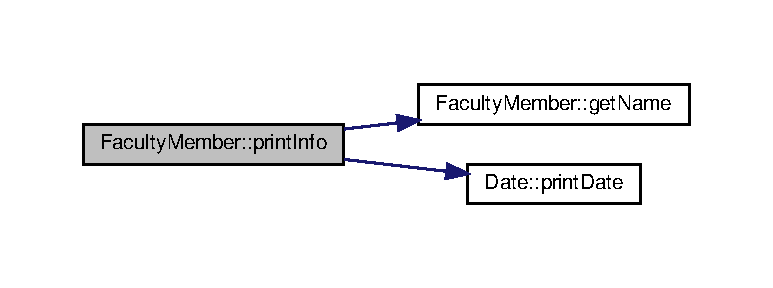
\includegraphics[width=350pt]{classFacultyMember_af07c814d58d1a2e309c74a0c57b95fd1_cgraph}
\end{center}
\end{figure}
\mbox{\Hypertarget{classFacultyMember_a25dc17f307ac885a7b3722a7685cb517}\label{classFacultyMember_a25dc17f307ac885a7b3722a7685cb517}} 
\index{Faculty\+Member@{Faculty\+Member}!set\+Address@{set\+Address}}
\index{set\+Address@{set\+Address}!Faculty\+Member@{Faculty\+Member}}
\subsubsection{\texorpdfstring{set\+Address()}{setAddress()}}
{\footnotesize\ttfamily void Faculty\+Member\+::set\+Address (\begin{DoxyParamCaption}\item[{std\+::string}]{address }\end{DoxyParamCaption})}

Sets the address of a faculty member. 
\begin{DoxyParams}{Parameters}
{\em address} & The address of a faculty member. \\
\hline
\end{DoxyParams}


Definition at line 113 of file Faculty\+Member.\+cpp.

\mbox{\Hypertarget{classFacultyMember_aceb0270b28a96e52cfe138c26f3936a4}\label{classFacultyMember_aceb0270b28a96e52cfe138c26f3936a4}} 
\index{Faculty\+Member@{Faculty\+Member}!set\+Cellphone\+Number@{set\+Cellphone\+Number}}
\index{set\+Cellphone\+Number@{set\+Cellphone\+Number}!Faculty\+Member@{Faculty\+Member}}
\subsubsection{\texorpdfstring{set\+Cellphone\+Number()}{setCellphoneNumber()}}
{\footnotesize\ttfamily void Faculty\+Member\+::set\+Cellphone\+Number (\begin{DoxyParamCaption}\item[{int}]{cellphone\+Number }\end{DoxyParamCaption})}

Sets the cellphone number of a faculty member. 
\begin{DoxyParams}{Parameters}
{\em cellphone\+Number} & The cellphone number of a faculty member. \\
\hline
\end{DoxyParams}


Definition at line 131 of file Faculty\+Member.\+cpp.

\mbox{\Hypertarget{classFacultyMember_acb54ae36938fc1b96bdb1ae8060c29c1}\label{classFacultyMember_acb54ae36938fc1b96bdb1ae8060c29c1}} 
\index{Faculty\+Member@{Faculty\+Member}!set\+Code@{set\+Code}}
\index{set\+Code@{set\+Code}!Faculty\+Member@{Faculty\+Member}}
\subsubsection{\texorpdfstring{set\+Code()}{setCode()}}
{\footnotesize\ttfamily void Faculty\+Member\+::set\+Code (\begin{DoxyParamCaption}\item[{int}]{code }\end{DoxyParamCaption})}

Sets the code of a faculty member. 
\begin{DoxyParams}{Parameters}
{\em code} & The code of a faculty member. \\
\hline
\end{DoxyParams}


Definition at line 140 of file Faculty\+Member.\+cpp.

\mbox{\Hypertarget{classFacultyMember_abec27c8af8bd8274a3ea560da0f12cbd}\label{classFacultyMember_abec27c8af8bd8274a3ea560da0f12cbd}} 
\index{Faculty\+Member@{Faculty\+Member}!set\+Date@{set\+Date}}
\index{set\+Date@{set\+Date}!Faculty\+Member@{Faculty\+Member}}
\subsubsection{\texorpdfstring{set\+Date()}{setDate()}}
{\footnotesize\ttfamily void Faculty\+Member\+::set\+Date (\begin{DoxyParamCaption}\item[{\hyperlink{classDate}{Date}}]{date }\end{DoxyParamCaption})}

Sets the date of a faculty member. 
\begin{DoxyParams}{Parameters}
{\em date} & The date of a faculty member. \\
\hline
\end{DoxyParams}


Definition at line 122 of file Faculty\+Member.\+cpp.

\mbox{\Hypertarget{classFacultyMember_a7e4ef8e1a740e7e46d17ed9df43bc5d8}\label{classFacultyMember_a7e4ef8e1a740e7e46d17ed9df43bc5d8}} 
\index{Faculty\+Member@{Faculty\+Member}!set\+Name@{set\+Name}}
\index{set\+Name@{set\+Name}!Faculty\+Member@{Faculty\+Member}}
\subsubsection{\texorpdfstring{set\+Name()}{setName()}}
{\footnotesize\ttfamily void Faculty\+Member\+::set\+Name (\begin{DoxyParamCaption}\item[{std\+::string}]{name }\end{DoxyParamCaption})}

Sets the name of a faculty member. 
\begin{DoxyParams}{Parameters}
{\em name} & The name of a faculty member. \\
\hline
\end{DoxyParams}


Definition at line 104 of file Faculty\+Member.\+cpp.



The documentation for this class was generated from the following files\+:\begin{DoxyCompactItemize}
\item 
include/Faculty\+Member.\+hpp\item 
src/Faculty\+Member.\+cpp\end{DoxyCompactItemize}

\hypertarget{classIntegratedMasters}{}\section{Integrated\+Masters Class Reference}
\label{classIntegratedMasters}\index{Integrated\+Masters@{Integrated\+Masters}}


Inheritance diagram for Integrated\+Masters\+:\nopagebreak
\begin{figure}[H]
\begin{center}
\leavevmode
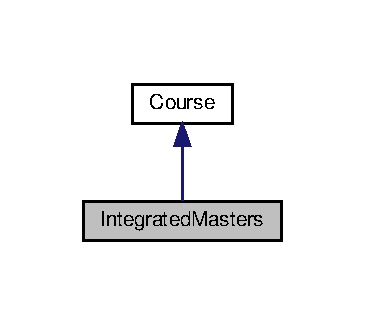
\includegraphics[width=175pt]{classIntegratedMasters__inherit__graph}
\end{center}
\end{figure}


Collaboration diagram for Integrated\+Masters\+:\nopagebreak
\begin{figure}[H]
\begin{center}
\leavevmode
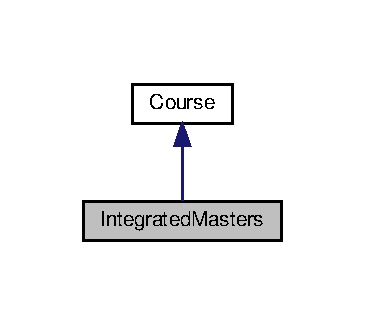
\includegraphics[width=175pt]{classIntegratedMasters__coll__graph}
\end{center}
\end{figure}
\subsection*{Public Member Functions}
\begin{DoxyCompactItemize}
\item 
\hyperlink{classIntegratedMasters_abb56fa7208cf3bb9ea74198c074e2dc8}{Integrated\+Masters} (unsigned int code, std\+::string name, std\+::map$<$ int, std\+::vector$<$ \hyperlink{classSubject}{Subject} $\ast$$>$$>$ curricular\+Plan, std\+::string director)
\item 
unsigned int \hyperlink{classIntegratedMasters_a8a126eac588aa68ed2895b589d34a7ed}{get\+Duration} () const
\item 
void \hyperlink{classIntegratedMasters_a71d4f5089e42207af1106604e316f155}{print\+Info} () const
\item 
void \hyperlink{classIntegratedMasters_a7be9fb139aef4a5b839bb6879de8cddb}{set\+Duration} (unsigned int d)
\item 
\mbox{\Hypertarget{classIntegratedMasters_aadff7d568166626c4fe151320399e643}\label{classIntegratedMasters_aadff7d568166626c4fe151320399e643}} 
void {\bfseries compated\+Information} (std\+::ofstream \&f)
\end{DoxyCompactItemize}
\subsection*{Additional Inherited Members}


\subsection{Detailed Description}


Definition at line 75 of file Course.\+hpp.



\subsection{Constructor \& Destructor Documentation}
\mbox{\Hypertarget{classIntegratedMasters_abb56fa7208cf3bb9ea74198c074e2dc8}\label{classIntegratedMasters_abb56fa7208cf3bb9ea74198c074e2dc8}} 
\index{Integrated\+Masters@{Integrated\+Masters}!Integrated\+Masters@{Integrated\+Masters}}
\index{Integrated\+Masters@{Integrated\+Masters}!Integrated\+Masters@{Integrated\+Masters}}
\subsubsection{\texorpdfstring{Integrated\+Masters()}{IntegratedMasters()}}
{\footnotesize\ttfamily Integrated\+Masters\+::\+Integrated\+Masters (\begin{DoxyParamCaption}\item[{unsigned int}]{code,  }\item[{std\+::string}]{name,  }\item[{std\+::map$<$ int, std\+::vector$<$ \hyperlink{classSubject}{Subject} $\ast$$>$$>$}]{curricular\+Plan,  }\item[{std\+::string}]{director }\end{DoxyParamCaption})}

Constructs an \hyperlink{classIntegratedMasters}{Integrated\+Masters} objects with every attribute value as parameters. 
\begin{DoxyParams}{Parameters}
{\em code} & The code of the course. \\
\hline
{\em name} & The name of the course. \\
\hline
{\em curricular\+Plan} & The curricular plan of the course. \\
\hline
{\em director} & The director of the course. \\
\hline
\end{DoxyParams}


Definition at line 196 of file Course.\+cpp.



\subsection{Member Function Documentation}
\mbox{\Hypertarget{classIntegratedMasters_a8a126eac588aa68ed2895b589d34a7ed}\label{classIntegratedMasters_a8a126eac588aa68ed2895b589d34a7ed}} 
\index{Integrated\+Masters@{Integrated\+Masters}!get\+Duration@{get\+Duration}}
\index{get\+Duration@{get\+Duration}!Integrated\+Masters@{Integrated\+Masters}}
\subsubsection{\texorpdfstring{get\+Duration()}{getDuration()}}
{\footnotesize\ttfamily unsigned int Integrated\+Masters\+::get\+Duration (\begin{DoxyParamCaption}{ }\end{DoxyParamCaption}) const\hspace{0.3cm}{\ttfamily [virtual]}}

Gets the duration of the course. \begin{DoxyReturn}{Returns}
The duration of the course. 
\end{DoxyReturn}


Implements \hyperlink{classCourse}{Course}.



Definition at line 278 of file Course.\+cpp.

\mbox{\Hypertarget{classIntegratedMasters_a71d4f5089e42207af1106604e316f155}\label{classIntegratedMasters_a71d4f5089e42207af1106604e316f155}} 
\index{Integrated\+Masters@{Integrated\+Masters}!print\+Info@{print\+Info}}
\index{print\+Info@{print\+Info}!Integrated\+Masters@{Integrated\+Masters}}
\subsubsection{\texorpdfstring{print\+Info()}{printInfo()}}
{\footnotesize\ttfamily void Integrated\+Masters\+::print\+Info (\begin{DoxyParamCaption}{ }\end{DoxyParamCaption}) const\hspace{0.3cm}{\ttfamily [virtual]}}

Prints the values of every attribute of the class. 

Reimplemented from \hyperlink{classCourse_a3248ecd5df196cf50ce379ec37758c59}{Course}.



Definition at line 207 of file Course.\+cpp.

\mbox{\Hypertarget{classIntegratedMasters_a7be9fb139aef4a5b839bb6879de8cddb}\label{classIntegratedMasters_a7be9fb139aef4a5b839bb6879de8cddb}} 
\index{Integrated\+Masters@{Integrated\+Masters}!set\+Duration@{set\+Duration}}
\index{set\+Duration@{set\+Duration}!Integrated\+Masters@{Integrated\+Masters}}
\subsubsection{\texorpdfstring{set\+Duration()}{setDuration()}}
{\footnotesize\ttfamily void Integrated\+Masters\+::set\+Duration (\begin{DoxyParamCaption}\item[{unsigned int}]{d }\end{DoxyParamCaption})\hspace{0.3cm}{\ttfamily [virtual]}}

Sets the duration of the course. 
\begin{DoxyParams}{Parameters}
{\em d} & The duration of the course. \\
\hline
\end{DoxyParams}


Implements \hyperlink{classCourse}{Course}.



Definition at line 216 of file Course.\+cpp.



The documentation for this class was generated from the following files\+:\begin{DoxyCompactItemize}
\item 
include/Course.\+hpp\item 
src/Course.\+cpp\end{DoxyCompactItemize}

\hypertarget{classInvalidCourse}{}\section{Invalid\+Course Class Reference}
\label{classInvalidCourse}\index{Invalid\+Course@{Invalid\+Course}}


Inheritance diagram for Invalid\+Course\+:\nopagebreak
\begin{figure}[H]
\begin{center}
\leavevmode
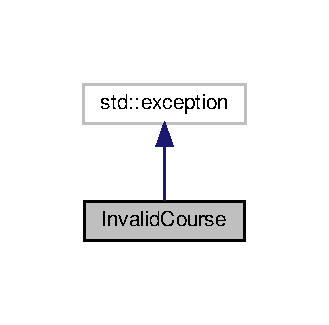
\includegraphics[width=158pt]{classInvalidCourse__inherit__graph}
\end{center}
\end{figure}


Collaboration diagram for Invalid\+Course\+:\nopagebreak
\begin{figure}[H]
\begin{center}
\leavevmode
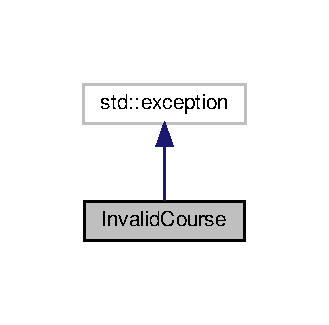
\includegraphics[width=158pt]{classInvalidCourse__coll__graph}
\end{center}
\end{figure}
\subsection*{Public Member Functions}
\begin{DoxyCompactItemize}
\item 
\mbox{\Hypertarget{classInvalidCourse_a7c63453c372463502e1c4ba9766d15dd}\label{classInvalidCourse_a7c63453c372463502e1c4ba9766d15dd}} 
{\bfseries Invalid\+Course} (int error\+\_\+code)
\item 
\mbox{\Hypertarget{classInvalidCourse_a103858b14f6b2e7e5b9cbf304cc1b1fd}\label{classInvalidCourse_a103858b14f6b2e7e5b9cbf304cc1b1fd}} 
virtual const char $\ast$ {\bfseries what} () const  throw ()
\end{DoxyCompactItemize}


\subsection{Detailed Description}


Definition at line 100 of file Course.\+hpp.



The documentation for this class was generated from the following file\+:\begin{DoxyCompactItemize}
\item 
include/Course.\+hpp\end{DoxyCompactItemize}

\hypertarget{classInvalidDate}{}\section{Invalid\+Date Class Reference}
\label{classInvalidDate}\index{Invalid\+Date@{Invalid\+Date}}


Inheritance diagram for Invalid\+Date\+:\nopagebreak
\begin{figure}[H]
\begin{center}
\leavevmode
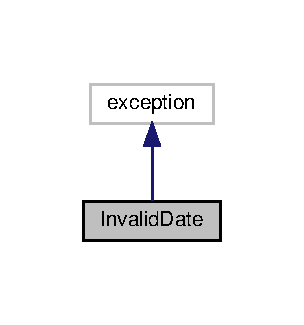
\includegraphics[width=146pt]{classInvalidDate__inherit__graph}
\end{center}
\end{figure}


Collaboration diagram for Invalid\+Date\+:\nopagebreak
\begin{figure}[H]
\begin{center}
\leavevmode
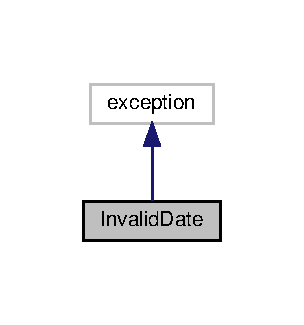
\includegraphics[width=146pt]{classInvalidDate__coll__graph}
\end{center}
\end{figure}
\subsection*{Public Member Functions}
\begin{DoxyCompactItemize}
\item 
\hyperlink{classInvalidDate_aec0b6360cdfe3c61278ac5ff668dc946}{Invalid\+Date} (int value, std\+::string wrong\+Parameter)
\item 
\hyperlink{classInvalidDate_acd3b0f4629f51807bd95a7530642d8f3}{Invalid\+Date} (int value, std\+::string wrong\+Parameter, int error\+\_\+code)
\item 
virtual const char $\ast$ \hyperlink{classInvalidDate_ae3a017e8f670ebc051f4bbcb5edae47f}{what} () const  throw ()
\item 
int \hyperlink{classInvalidDate_af05b8106788ddffe0730431d14eb206f}{get\+Value} ()
\item 
std\+::string \hyperlink{classInvalidDate_ac88bde221f49a16107a7cea66e214819}{get\+Parameter} ()
\end{DoxyCompactItemize}


\subsection{Detailed Description}


Definition at line 38 of file Date.\+hpp.



\subsection{Constructor \& Destructor Documentation}
\mbox{\Hypertarget{classInvalidDate_aec0b6360cdfe3c61278ac5ff668dc946}\label{classInvalidDate_aec0b6360cdfe3c61278ac5ff668dc946}} 
\index{Invalid\+Date@{Invalid\+Date}!Invalid\+Date@{Invalid\+Date}}
\index{Invalid\+Date@{Invalid\+Date}!Invalid\+Date@{Invalid\+Date}}
\subsubsection{\texorpdfstring{Invalid\+Date()}{InvalidDate()}\hspace{0.1cm}{\footnotesize\ttfamily [1/2]}}
{\footnotesize\ttfamily Invalid\+Date\+::\+Invalid\+Date (\begin{DoxyParamCaption}\item[{int}]{value,  }\item[{std\+::string}]{wrong\+Parameter }\end{DoxyParamCaption})}

Constructs an \hyperlink{classInvalidDate}{Invalid\+Date} object. 
\begin{DoxyParams}{Parameters}
{\em value} & The value that is wrong on the date. \\
\hline
{\em wrong\+Parameter} & The name of the wrong parameter. \\
\hline
\end{DoxyParams}


Definition at line 8 of file Date.\+cpp.

\mbox{\Hypertarget{classInvalidDate_acd3b0f4629f51807bd95a7530642d8f3}\label{classInvalidDate_acd3b0f4629f51807bd95a7530642d8f3}} 
\index{Invalid\+Date@{Invalid\+Date}!Invalid\+Date@{Invalid\+Date}}
\index{Invalid\+Date@{Invalid\+Date}!Invalid\+Date@{Invalid\+Date}}
\subsubsection{\texorpdfstring{Invalid\+Date()}{InvalidDate()}\hspace{0.1cm}{\footnotesize\ttfamily [2/2]}}
{\footnotesize\ttfamily Invalid\+Date\+::\+Invalid\+Date (\begin{DoxyParamCaption}\item[{int}]{value,  }\item[{std\+::string}]{wrong\+Parameter,  }\item[{int}]{error\+\_\+code }\end{DoxyParamCaption})}

Constructs an \hyperlink{classInvalidDate}{Invalid\+Date} object. 
\begin{DoxyParams}{Parameters}
{\em value} & The value that is wrong on the date. \\
\hline
{\em wrong\+Parameter} & The name of the wrong parameter. \\
\hline
{\em error\+\_\+code} & The error code. \\
\hline
\end{DoxyParams}


Definition at line 20 of file Date.\+cpp.



\subsection{Member Function Documentation}
\mbox{\Hypertarget{classInvalidDate_ac88bde221f49a16107a7cea66e214819}\label{classInvalidDate_ac88bde221f49a16107a7cea66e214819}} 
\index{Invalid\+Date@{Invalid\+Date}!get\+Parameter@{get\+Parameter}}
\index{get\+Parameter@{get\+Parameter}!Invalid\+Date@{Invalid\+Date}}
\subsubsection{\texorpdfstring{get\+Parameter()}{getParameter()}}
{\footnotesize\ttfamily string Invalid\+Date\+::get\+Parameter (\begin{DoxyParamCaption}{ }\end{DoxyParamCaption})}

Gets the name of the wrong parameter. \begin{DoxyReturn}{Returns}
The name of the wrong parameter. 
\end{DoxyReturn}


Definition at line 59 of file Date.\+cpp.

\mbox{\Hypertarget{classInvalidDate_af05b8106788ddffe0730431d14eb206f}\label{classInvalidDate_af05b8106788ddffe0730431d14eb206f}} 
\index{Invalid\+Date@{Invalid\+Date}!get\+Value@{get\+Value}}
\index{get\+Value@{get\+Value}!Invalid\+Date@{Invalid\+Date}}
\subsubsection{\texorpdfstring{get\+Value()}{getValue()}}
{\footnotesize\ttfamily int Invalid\+Date\+::get\+Value (\begin{DoxyParamCaption}{ }\end{DoxyParamCaption})}

Gets the value of the \hyperlink{classInvalidDate}{Invalid\+Date} object. \begin{DoxyReturn}{Returns}
The value of the date. 
\end{DoxyReturn}


Definition at line 50 of file Date.\+cpp.

\mbox{\Hypertarget{classInvalidDate_ae3a017e8f670ebc051f4bbcb5edae47f}\label{classInvalidDate_ae3a017e8f670ebc051f4bbcb5edae47f}} 
\index{Invalid\+Date@{Invalid\+Date}!what@{what}}
\index{what@{what}!Invalid\+Date@{Invalid\+Date}}
\subsubsection{\texorpdfstring{what()}{what()}}
{\footnotesize\ttfamily const char $\ast$ Invalid\+Date\+::what (\begin{DoxyParamCaption}{ }\end{DoxyParamCaption}) const throw  ) \hspace{0.3cm}{\ttfamily [virtual]}}

Returns the type of error of the class \hyperlink{classInvalidDate}{Invalid\+Date}. \begin{DoxyReturn}{Returns}
The type of error. 
\end{DoxyReturn}


Definition at line 31 of file Date.\+cpp.



The documentation for this class was generated from the following files\+:\begin{DoxyCompactItemize}
\item 
include/Date.\+hpp\item 
src/Date.\+cpp\end{DoxyCompactItemize}

\hypertarget{classInvalidDepartment}{}\section{Invalid\+Department Class Reference}
\label{classInvalidDepartment}\index{Invalid\+Department@{Invalid\+Department}}


Inheritance diagram for Invalid\+Department\+:\nopagebreak
\begin{figure}[H]
\begin{center}
\leavevmode
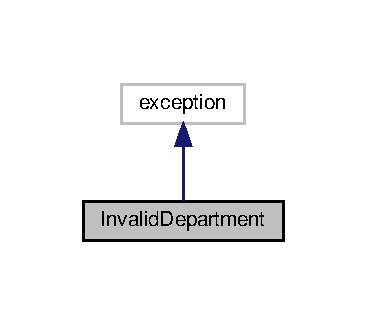
\includegraphics[width=176pt]{classInvalidDepartment__inherit__graph}
\end{center}
\end{figure}


Collaboration diagram for Invalid\+Department\+:\nopagebreak
\begin{figure}[H]
\begin{center}
\leavevmode
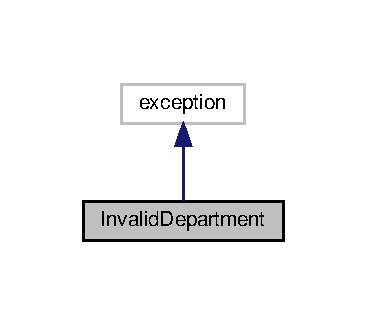
\includegraphics[width=176pt]{classInvalidDepartment__coll__graph}
\end{center}
\end{figure}
\subsection*{Public Member Functions}
\begin{DoxyCompactItemize}
\item 
\mbox{\Hypertarget{classInvalidDepartment_ae3c8a8a0d280123ef5225355512bd080}\label{classInvalidDepartment_ae3c8a8a0d280123ef5225355512bd080}} 
{\bfseries Invalid\+Department} (int error\+\_\+code)
\item 
\mbox{\Hypertarget{classInvalidDepartment_a5cfcc2e3de7111deca40f63619cd850f}\label{classInvalidDepartment_a5cfcc2e3de7111deca40f63619cd850f}} 
virtual const char $\ast$ {\bfseries what} () const  throw ()
\end{DoxyCompactItemize}


\subsection{Detailed Description}


Definition at line 35 of file Department.\+hpp.



The documentation for this class was generated from the following file\+:\begin{DoxyCompactItemize}
\item 
include/Department.\+hpp\end{DoxyCompactItemize}

\hypertarget{classInvalidFaculty}{}\section{Invalid\+Faculty Class Reference}
\label{classInvalidFaculty}\index{Invalid\+Faculty@{Invalid\+Faculty}}


Inheritance diagram for Invalid\+Faculty\+:\nopagebreak
\begin{figure}[H]
\begin{center}
\leavevmode
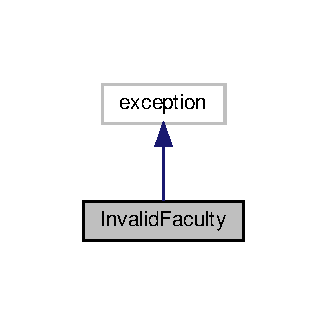
\includegraphics[width=157pt]{classInvalidFaculty__inherit__graph}
\end{center}
\end{figure}


Collaboration diagram for Invalid\+Faculty\+:\nopagebreak
\begin{figure}[H]
\begin{center}
\leavevmode
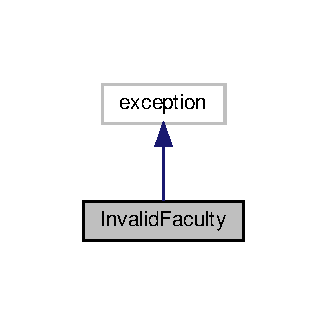
\includegraphics[width=157pt]{classInvalidFaculty__coll__graph}
\end{center}
\end{figure}
\subsection*{Public Member Functions}
\begin{DoxyCompactItemize}
\item 
\mbox{\Hypertarget{classInvalidFaculty_adc180b691b52cb5da0ce2a4f02e873a4}\label{classInvalidFaculty_adc180b691b52cb5da0ce2a4f02e873a4}} 
{\bfseries Invalid\+Faculty} (int error\+\_\+code)
\item 
\mbox{\Hypertarget{classInvalidFaculty_a11cddd616dd48218975f14a625ca3906}\label{classInvalidFaculty_a11cddd616dd48218975f14a625ca3906}} 
virtual const char $\ast$ {\bfseries what} () const  throw ()
\end{DoxyCompactItemize}


\subsection{Detailed Description}


Definition at line 85 of file Faculty.\+hpp.



The documentation for this class was generated from the following file\+:\begin{DoxyCompactItemize}
\item 
include/Faculty.\+hpp\end{DoxyCompactItemize}

\hypertarget{classInvalidFacultyMember}{}\section{Invalid\+Faculty\+Member Class Reference}
\label{classInvalidFacultyMember}\index{Invalid\+Faculty\+Member@{Invalid\+Faculty\+Member}}


Inheritance diagram for Invalid\+Faculty\+Member\+:\nopagebreak
\begin{figure}[H]
\begin{center}
\leavevmode
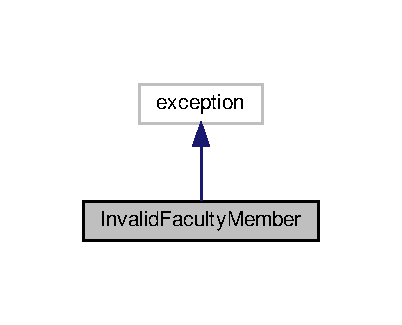
\includegraphics[width=193pt]{classInvalidFacultyMember__inherit__graph}
\end{center}
\end{figure}


Collaboration diagram for Invalid\+Faculty\+Member\+:\nopagebreak
\begin{figure}[H]
\begin{center}
\leavevmode
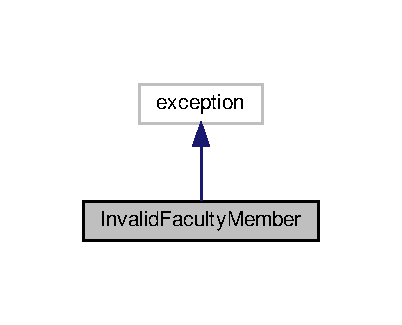
\includegraphics[width=193pt]{classInvalidFacultyMember__coll__graph}
\end{center}
\end{figure}
\subsection*{Public Member Functions}
\begin{DoxyCompactItemize}
\item 
\mbox{\Hypertarget{classInvalidFacultyMember_ab037a7ef14d1c0fe3b16b7fbeb47f9d4}\label{classInvalidFacultyMember_ab037a7ef14d1c0fe3b16b7fbeb47f9d4}} 
{\bfseries Invalid\+Faculty\+Member} (int error\+\_\+code)
\item 
\mbox{\Hypertarget{classInvalidFacultyMember_ac03a8c3d9a4b01765b14bf7fabd5ff8a}\label{classInvalidFacultyMember_ac03a8c3d9a4b01765b14bf7fabd5ff8a}} 
virtual const char $\ast$ {\bfseries what} () const  throw ()
\end{DoxyCompactItemize}


\subsection{Detailed Description}


Definition at line 143 of file Faculty\+Member.\+hpp.



The documentation for this class was generated from the following file\+:\begin{DoxyCompactItemize}
\item 
include/Faculty\+Member.\+hpp\end{DoxyCompactItemize}

\hypertarget{classInvalidSubject}{}\section{Invalid\+Subject Class Reference}
\label{classInvalidSubject}\index{Invalid\+Subject@{Invalid\+Subject}}


Inheritance diagram for Invalid\+Subject\+:\nopagebreak
\begin{figure}[H]
\begin{center}
\leavevmode
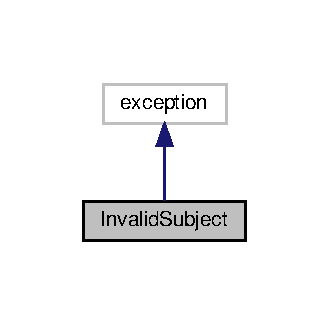
\includegraphics[width=158pt]{classInvalidSubject__inherit__graph}
\end{center}
\end{figure}


Collaboration diagram for Invalid\+Subject\+:\nopagebreak
\begin{figure}[H]
\begin{center}
\leavevmode
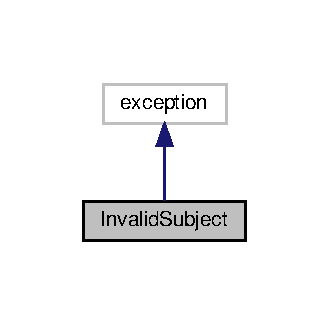
\includegraphics[width=158pt]{classInvalidSubject__coll__graph}
\end{center}
\end{figure}
\subsection*{Public Member Functions}
\begin{DoxyCompactItemize}
\item 
\mbox{\Hypertarget{classInvalidSubject_accec9773905ac5c51bbc73eb02fffe7b}\label{classInvalidSubject_accec9773905ac5c51bbc73eb02fffe7b}} 
{\bfseries Invalid\+Subject} (int error\+\_\+code)
\item 
\mbox{\Hypertarget{classInvalidSubject_a41dcf5036269f11d1d6918950c8f0997}\label{classInvalidSubject_a41dcf5036269f11d1d6918950c8f0997}} 
virtual const char $\ast$ {\bfseries what} () const  throw ()
\end{DoxyCompactItemize}


\subsection{Detailed Description}


Definition at line 66 of file Subject.\+hpp.



The documentation for this class was generated from the following file\+:\begin{DoxyCompactItemize}
\item 
include/Subject.\+hpp\end{DoxyCompactItemize}

\hypertarget{classMasters}{}\section{Masters Class Reference}
\label{classMasters}\index{Masters@{Masters}}


Inheritance diagram for Masters\+:\nopagebreak
\begin{figure}[H]
\begin{center}
\leavevmode
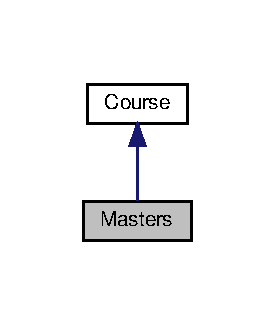
\includegraphics[width=132pt]{classMasters__inherit__graph}
\end{center}
\end{figure}


Collaboration diagram for Masters\+:\nopagebreak
\begin{figure}[H]
\begin{center}
\leavevmode
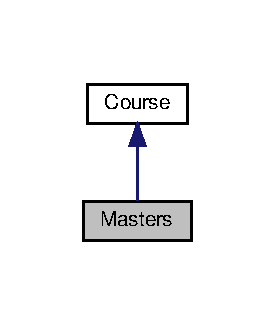
\includegraphics[width=132pt]{classMasters__coll__graph}
\end{center}
\end{figure}
\subsection*{Public Member Functions}
\begin{DoxyCompactItemize}
\item 
\hyperlink{classMasters_a37bef5483363064f8253ac2532e44904}{Masters} (unsigned int code, std\+::string name, std\+::map$<$ int, std\+::vector$<$ \hyperlink{classSubject}{Subject} $\ast$$>$$>$ curricular\+Plan, std\+::string director)
\item 
unsigned int \hyperlink{classMasters_a1ce9d04336172b5ea01e0fc397329f7c}{get\+Duration} () const
\item 
void \hyperlink{classMasters_a72034d4ad86c3d62c755ad04228d09da}{print\+Info} () const
\item 
void \hyperlink{classMasters_af80b6665ac5a0f5fb189da1fd636b0fb}{set\+Duration} (unsigned int d)
\item 
\mbox{\Hypertarget{classMasters_a2e3fe30a654585e98ade65c560f80238}\label{classMasters_a2e3fe30a654585e98ade65c560f80238}} 
void {\bfseries compated\+Information} (std\+::ofstream \&f)
\end{DoxyCompactItemize}
\subsection*{Additional Inherited Members}


\subsection{Detailed Description}


Definition at line 58 of file Course.\+hpp.



\subsection{Constructor \& Destructor Documentation}
\mbox{\Hypertarget{classMasters_a37bef5483363064f8253ac2532e44904}\label{classMasters_a37bef5483363064f8253ac2532e44904}} 
\index{Masters@{Masters}!Masters@{Masters}}
\index{Masters@{Masters}!Masters@{Masters}}
\subsubsection{\texorpdfstring{Masters()}{Masters()}}
{\footnotesize\ttfamily Masters\+::\+Masters (\begin{DoxyParamCaption}\item[{unsigned int}]{code,  }\item[{std\+::string}]{name,  }\item[{std\+::map$<$ int, std\+::vector$<$ \hyperlink{classSubject}{Subject} $\ast$$>$$>$}]{curricular\+Plan,  }\item[{std\+::string}]{director }\end{DoxyParamCaption})}

Constructs an object Master with every attribute as parameters. 
\begin{DoxyParams}{Parameters}
{\em code} & The code of the course. \\
\hline
{\em name} & The name of the course. \\
\hline
{\em curricular\+Plan} & The curricular plan of the course. \\
\hline
{\em director} & The director of the course. \\
\hline
\end{DoxyParams}


Definition at line 164 of file Course.\+cpp.



\subsection{Member Function Documentation}
\mbox{\Hypertarget{classMasters_a1ce9d04336172b5ea01e0fc397329f7c}\label{classMasters_a1ce9d04336172b5ea01e0fc397329f7c}} 
\index{Masters@{Masters}!get\+Duration@{get\+Duration}}
\index{get\+Duration@{get\+Duration}!Masters@{Masters}}
\subsubsection{\texorpdfstring{get\+Duration()}{getDuration()}}
{\footnotesize\ttfamily unsigned int Masters\+::get\+Duration (\begin{DoxyParamCaption}{ }\end{DoxyParamCaption}) const\hspace{0.3cm}{\ttfamily [virtual]}}

Gets the duration of the course. \begin{DoxyReturn}{Returns}
The duration of the course. 
\end{DoxyReturn}


Implements \hyperlink{classCourse}{Course}.



Definition at line 269 of file Course.\+cpp.

\mbox{\Hypertarget{classMasters_a72034d4ad86c3d62c755ad04228d09da}\label{classMasters_a72034d4ad86c3d62c755ad04228d09da}} 
\index{Masters@{Masters}!print\+Info@{print\+Info}}
\index{print\+Info@{print\+Info}!Masters@{Masters}}
\subsubsection{\texorpdfstring{print\+Info()}{printInfo()}}
{\footnotesize\ttfamily void Masters\+::print\+Info (\begin{DoxyParamCaption}{ }\end{DoxyParamCaption}) const\hspace{0.3cm}{\ttfamily [virtual]}}

Prints the values of every attribute of the class. 

Reimplemented from \hyperlink{classCourse_a3248ecd5df196cf50ce379ec37758c59}{Course}.



Definition at line 174 of file Course.\+cpp.

\mbox{\Hypertarget{classMasters_af80b6665ac5a0f5fb189da1fd636b0fb}\label{classMasters_af80b6665ac5a0f5fb189da1fd636b0fb}} 
\index{Masters@{Masters}!set\+Duration@{set\+Duration}}
\index{set\+Duration@{set\+Duration}!Masters@{Masters}}
\subsubsection{\texorpdfstring{set\+Duration()}{setDuration()}}
{\footnotesize\ttfamily void Masters\+::set\+Duration (\begin{DoxyParamCaption}\item[{unsigned int}]{d }\end{DoxyParamCaption})\hspace{0.3cm}{\ttfamily [virtual]}}

Sets the duration of the course. 
\begin{DoxyParams}{Parameters}
{\em d} & The duration of the course. \\
\hline
\end{DoxyParams}


Implements \hyperlink{classCourse}{Course}.



Definition at line 183 of file Course.\+cpp.



The documentation for this class was generated from the following files\+:\begin{DoxyCompactItemize}
\item 
include/Course.\+hpp\item 
src/Course.\+cpp\end{DoxyCompactItemize}

\hypertarget{classStaff}{}\section{Staff Class Reference}
\label{classStaff}\index{Staff@{Staff}}


Inheritance diagram for Staff\+:\nopagebreak
\begin{figure}[H]
\begin{center}
\leavevmode
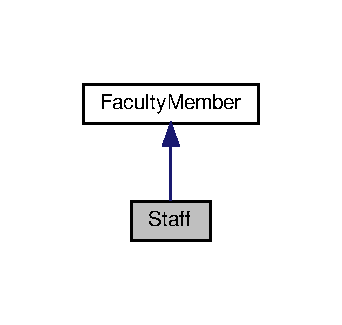
\includegraphics[width=164pt]{classStaff__inherit__graph}
\end{center}
\end{figure}


Collaboration diagram for Staff\+:\nopagebreak
\begin{figure}[H]
\begin{center}
\leavevmode
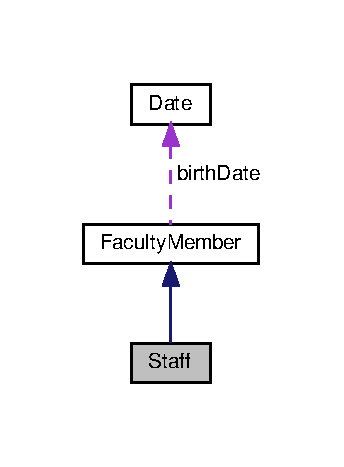
\includegraphics[width=165pt]{classStaff__coll__graph}
\end{center}
\end{figure}
\subsection*{Public Member Functions}
\begin{DoxyCompactItemize}
\item 
\hyperlink{classStaff_af590aec2ea7c88fd95486c2fa5f92b2f}{Staff} (std\+::string name, std\+::string address, \hyperlink{classDate}{Date} birth\+Date, int cellphone\+Number, int code, int tax\+Payer\+Number, int salary, std\+::string field\+Of\+Work)
\item 
\mbox{\Hypertarget{classStaff_ae763bc48a07f1195bc31610bb6db583b}\label{classStaff_ae763bc48a07f1195bc31610bb6db583b}} 
int {\bfseries get\+Taxpayer\+Number} () const
\item 
\mbox{\Hypertarget{classStaff_a6a60b9d148150ac0bda240209ab5443c}\label{classStaff_a6a60b9d148150ac0bda240209ab5443c}} 
int {\bfseries get\+Salary} () const
\item 
\mbox{\Hypertarget{classStaff_a676f998076ace5103cf199004ed6f898}\label{classStaff_a676f998076ace5103cf199004ed6f898}} 
std\+::string {\bfseries get\+Field\+Of\+Work} () const
\item 
void \hyperlink{classStaff_a3b9babe4708b787b8aeb4d02be4ba1eb}{print\+Info} () const
\item 
void \hyperlink{classStaff_a383d6f3eeebdbf7fd7ff86f4e43bde99}{set\+Taxpayer\+Number} (int number)
\item 
void \hyperlink{classStaff_a70d472e604f726f11bd01bfe325b8216}{set\+Salary} (int salary)
\item 
void \hyperlink{classStaff_a3522c4036c9fcc08d2cd2ad4032ef507}{set\+Field\+Of\+Work} (std\+::string field)
\item 
\mbox{\Hypertarget{classStaff_a54ca19b398f976ce2524256d766a0ec9}\label{classStaff_a54ca19b398f976ce2524256d766a0ec9}} 
void {\bfseries compated\+Information} (std\+::ofstream \&f)
\end{DoxyCompactItemize}
\subsection*{Additional Inherited Members}


\subsection{Detailed Description}


Definition at line 94 of file Faculty\+Member.\+hpp.



\subsection{Constructor \& Destructor Documentation}
\mbox{\Hypertarget{classStaff_af590aec2ea7c88fd95486c2fa5f92b2f}\label{classStaff_af590aec2ea7c88fd95486c2fa5f92b2f}} 
\index{Staff@{Staff}!Staff@{Staff}}
\index{Staff@{Staff}!Staff@{Staff}}
\subsubsection{\texorpdfstring{Staff()}{Staff()}}
{\footnotesize\ttfamily Staff\+::\+Staff (\begin{DoxyParamCaption}\item[{std\+::string}]{name,  }\item[{std\+::string}]{address,  }\item[{\hyperlink{classDate}{Date}}]{birth\+Date,  }\item[{int}]{cellphone\+Number,  }\item[{int}]{code,  }\item[{int}]{tax\+Payer\+Number,  }\item[{int}]{salary,  }\item[{std\+::string}]{field\+Of\+Work }\end{DoxyParamCaption})}

Constructs a \hyperlink{classTeacher}{Teacher} object with all the attribute values as parameters 
\begin{DoxyParams}{Parameters}
{\em name} & The name of the teacher \\
\hline
{\em address} & The address of the teacher \\
\hline
{\em birth\+Date} & The birth date of the teacher \\
\hline
{\em cellphone\+Number} & The cellphone number of the teacher \\
\hline
{\em code} & The code of the teacher \\
\hline
{\em tax\+Payer\+Number} & The taxpayer number of the teacher \\
\hline
{\em salary} & The salary of the teacher \\
\hline
{\em field\+Of\+Work} & The field of work of the teacher \\
\hline
\end{DoxyParams}


Definition at line 427 of file Faculty\+Member.\+cpp.



\subsection{Member Function Documentation}
\mbox{\Hypertarget{classStaff_a3b9babe4708b787b8aeb4d02be4ba1eb}\label{classStaff_a3b9babe4708b787b8aeb4d02be4ba1eb}} 
\index{Staff@{Staff}!print\+Info@{print\+Info}}
\index{print\+Info@{print\+Info}!Staff@{Staff}}
\subsubsection{\texorpdfstring{print\+Info()}{printInfo()}}
{\footnotesize\ttfamily void Staff\+::print\+Info (\begin{DoxyParamCaption}{ }\end{DoxyParamCaption}) const\hspace{0.3cm}{\ttfamily [virtual]}}

Prints the infomration of the staff member, that is, the values of all its attributes 

Reimplemented from \hyperlink{classFacultyMember_af07c814d58d1a2e309c74a0c57b95fd1}{Faculty\+Member}.



Definition at line 455 of file Faculty\+Member.\+cpp.

\mbox{\Hypertarget{classStaff_a3522c4036c9fcc08d2cd2ad4032ef507}\label{classStaff_a3522c4036c9fcc08d2cd2ad4032ef507}} 
\index{Staff@{Staff}!set\+Field\+Of\+Work@{set\+Field\+Of\+Work}}
\index{set\+Field\+Of\+Work@{set\+Field\+Of\+Work}!Staff@{Staff}}
\subsubsection{\texorpdfstring{set\+Field\+Of\+Work()}{setFieldOfWork()}}
{\footnotesize\ttfamily void Staff\+::set\+Field\+Of\+Work (\begin{DoxyParamCaption}\item[{std\+::string}]{field }\end{DoxyParamCaption})}

Sets the field of work of the staff member 
\begin{DoxyParams}{Parameters}
{\em field} & The field of work of the staff member \\
\hline
\end{DoxyParams}


Definition at line 484 of file Faculty\+Member.\+cpp.

Here is the call graph for this function\+:\nopagebreak
\begin{figure}[H]
\begin{center}
\leavevmode
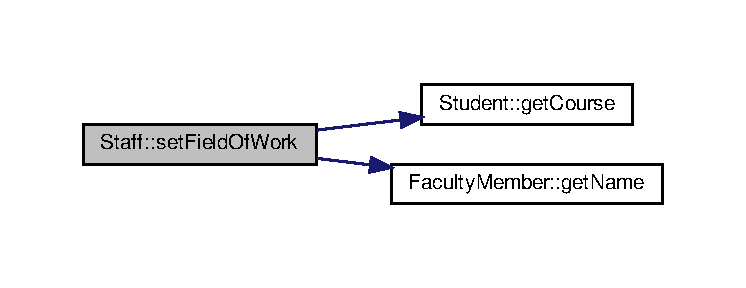
\includegraphics[width=350pt]{classStaff_a3522c4036c9fcc08d2cd2ad4032ef507_cgraph}
\end{center}
\end{figure}
\mbox{\Hypertarget{classStaff_a70d472e604f726f11bd01bfe325b8216}\label{classStaff_a70d472e604f726f11bd01bfe325b8216}} 
\index{Staff@{Staff}!set\+Salary@{set\+Salary}}
\index{set\+Salary@{set\+Salary}!Staff@{Staff}}
\subsubsection{\texorpdfstring{set\+Salary()}{setSalary()}}
{\footnotesize\ttfamily void Staff\+::set\+Salary (\begin{DoxyParamCaption}\item[{int}]{salary }\end{DoxyParamCaption})}

Sets the salary of the staff member 
\begin{DoxyParams}{Parameters}
{\em salary} & The salary of the staff member \\
\hline
\end{DoxyParams}


Definition at line 475 of file Faculty\+Member.\+cpp.

\mbox{\Hypertarget{classStaff_a383d6f3eeebdbf7fd7ff86f4e43bde99}\label{classStaff_a383d6f3eeebdbf7fd7ff86f4e43bde99}} 
\index{Staff@{Staff}!set\+Taxpayer\+Number@{set\+Taxpayer\+Number}}
\index{set\+Taxpayer\+Number@{set\+Taxpayer\+Number}!Staff@{Staff}}
\subsubsection{\texorpdfstring{set\+Taxpayer\+Number()}{setTaxpayerNumber()}}
{\footnotesize\ttfamily void Staff\+::set\+Taxpayer\+Number (\begin{DoxyParamCaption}\item[{int}]{number }\end{DoxyParamCaption})}

Sets the taxpayer number of the staff member 
\begin{DoxyParams}{Parameters}
{\em number} & The taxpayer number \\
\hline
\end{DoxyParams}


Definition at line 466 of file Faculty\+Member.\+cpp.



The documentation for this class was generated from the following files\+:\begin{DoxyCompactItemize}
\item 
include/Faculty\+Member.\+hpp\item 
src/Faculty\+Member.\+cpp\end{DoxyCompactItemize}

\hypertarget{structStaffPtrHash}{}\section{Staff\+Ptr\+Hash Struct Reference}
\label{structStaffPtrHash}\index{Staff\+Ptr\+Hash@{Staff\+Ptr\+Hash}}
\subsection*{Public Member Functions}
\begin{DoxyCompactItemize}
\item 
\mbox{\Hypertarget{structStaffPtrHash_af25389000e72b90bdcaf0ffc768d2256}\label{structStaffPtrHash_af25389000e72b90bdcaf0ffc768d2256}} 
int {\bfseries operator()} (const \hyperlink{classFacultyMember}{Faculty\+Member} \&student) const
\item 
\mbox{\Hypertarget{structStaffPtrHash_af174a2a12736391fb476cecf87506149}\label{structStaffPtrHash_af174a2a12736391fb476cecf87506149}} 
bool {\bfseries operator()} (const \hyperlink{classFacultyMember}{Faculty\+Member} \&student1, const \hyperlink{classFacultyMember}{Faculty\+Member} \&student2) const
\end{DoxyCompactItemize}


\subsection{Detailed Description}


Definition at line 13 of file Faculty.\+hpp.



The documentation for this struct was generated from the following file\+:\begin{DoxyCompactItemize}
\item 
include/Faculty.\+hpp\end{DoxyCompactItemize}

\hypertarget{classStudent}{}\section{Student Class Reference}
\label{classStudent}\index{Student@{Student}}


Inheritance diagram for Student\+:\nopagebreak
\begin{figure}[H]
\begin{center}
\leavevmode
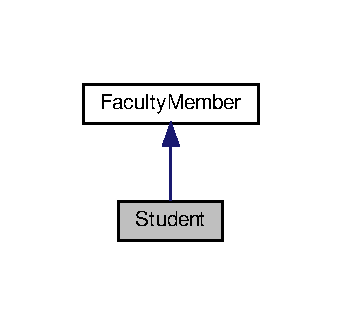
\includegraphics[width=164pt]{classStudent__inherit__graph}
\end{center}
\end{figure}


Collaboration diagram for Student\+:\nopagebreak
\begin{figure}[H]
\begin{center}
\leavevmode
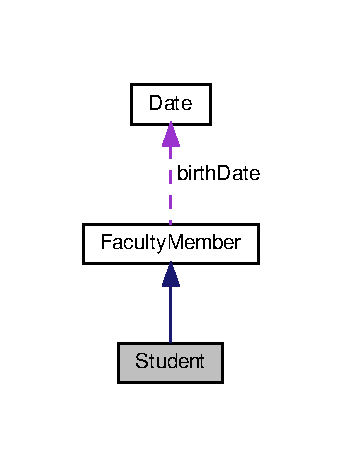
\includegraphics[width=165pt]{classStudent__coll__graph}
\end{center}
\end{figure}
\subsection*{Public Member Functions}
\begin{DoxyCompactItemize}
\item 
\mbox{\Hypertarget{classStudent_a180b54eea798e901422c7763b39aca67}\label{classStudent_a180b54eea798e901422c7763b39aca67}} 
{\bfseries Student} (std\+::string name, int course)
\item 
\hyperlink{classStudent_a048addf53c9fe5b126ec7656fbe701ad}{Student} (std\+::string name, std\+::string address, \hyperlink{classDate}{Date} birth\+Date, int cellphone\+Number, int code, int course, float average)
\item 
std\+::vector$<$ \hyperlink{classSubject}{Subject} $>$ \hyperlink{classStudent_a5db626d71418122132a534983d2a9c06}{get\+Subjects\+Taken} () const
\item 
void \hyperlink{classStudent_a0d882d0880d67c5d8b8df3cfe4ceec16}{add\+Subject\+Taken} (\hyperlink{classSubject}{Subject} c)
\item 
float \hyperlink{classStudent_a4bb700692481cee418c225d9fd27317d}{calculate\+Average} ()
\item 
void \hyperlink{classStudent_a3567f5c4220ffa88a8855998b3b99b43}{print\+Info} () const
\item 
void \hyperlink{classStudent_af7affdfd5b1b9e4d8c8d1fcb1e2cc631}{set\+Course} (int course)
\item 
void \hyperlink{classStudent_a2a24ebdce323c9cea4060b1cd9d343c9}{set\+Subjects\+Taken} (std\+::vector$<$ \hyperlink{classSubject}{Subject} $>$ subjects)
\item 
int \hyperlink{classStudent_a7ca1414a43b0c0194defe9a7929567a2}{get\+Course} () const
\item 
bool \hyperlink{classStudent_aabc24d469d7206a621fa154b3578d9e0}{operator$<$} (const \hyperlink{classStudent}{Student} \&s) const
\begin{DoxyCompactList}\small\item\em Returns the smallest student according to their average, curricular year and birthdate, respectively. \end{DoxyCompactList}\item 
unsigned int \hyperlink{classStudent_a40e4932da73265df93cf942d162c41b3}{get\+Curricular\+Year} () const
\begin{DoxyCompactList}\small\item\em Returns the curricular year of a student. \end{DoxyCompactList}\item 
\mbox{\Hypertarget{classStudent_ab0452be33ce4d8d991c716302c8a6b2d}\label{classStudent_ab0452be33ce4d8d991c716302c8a6b2d}} 
void {\bfseries set\+Curricular\+Year} (unsigned int curricular\+Year)
\item 
void \hyperlink{classStudent_a5b0b522fd636bfc266a08129a8784a0a}{set\+Average} (float average)
\begin{DoxyCompactList}\small\item\em Sets the average of a student. \end{DoxyCompactList}\item 
float \hyperlink{classStudent_a0d7d2e908da7c3d4b7d1fd7fb4bccf6c}{get\+Average} ()
\begin{DoxyCompactList}\small\item\em Gets the average of the student. \end{DoxyCompactList}\item 
\mbox{\Hypertarget{classStudent_aa5477568333bf5c85f5bf6a67d44580e}\label{classStudent_aa5477568333bf5c85f5bf6a67d44580e}} 
bool {\bfseries operator==} (const \hyperlink{classStudent}{Student} \&s1) const
\item 
\mbox{\Hypertarget{classStudent_a28d807df5f7ed8d39c9de19d6266ba82}\label{classStudent_a28d807df5f7ed8d39c9de19d6266ba82}} 
void {\bfseries compated\+Information} (std\+::ofstream \&f)
\end{DoxyCompactItemize}
\subsection*{Friends}
\begin{DoxyCompactItemize}
\item 
\mbox{\Hypertarget{classStudent_aba7f21809ffa875b1e9bf8aa756c0ab2}\label{classStudent_aba7f21809ffa875b1e9bf8aa756c0ab2}} 
class {\bfseries Student\+Ptr}
\end{DoxyCompactItemize}
\subsection*{Additional Inherited Members}


\subsection{Detailed Description}


Definition at line 41 of file Faculty\+Member.\+hpp.



\subsection{Constructor \& Destructor Documentation}
\mbox{\Hypertarget{classStudent_a048addf53c9fe5b126ec7656fbe701ad}\label{classStudent_a048addf53c9fe5b126ec7656fbe701ad}} 
\index{Student@{Student}!Student@{Student}}
\index{Student@{Student}!Student@{Student}}
\subsubsection{\texorpdfstring{Student()}{Student()}}
{\footnotesize\ttfamily Student\+::\+Student (\begin{DoxyParamCaption}\item[{std\+::string}]{name,  }\item[{std\+::string}]{address,  }\item[{\hyperlink{classDate}{Date}}]{birth\+Date,  }\item[{int}]{cellphone\+Number,  }\item[{int}]{code,  }\item[{int}]{course,  }\item[{float}]{average }\end{DoxyParamCaption})}

Constructs a \hyperlink{classStudent}{Student} object with all the attribute values of the class as parameters. 
\begin{DoxyParams}{Parameters}
{\em name} & The name of a student. \\
\hline
{\em address} & The address of a student. \\
\hline
{\em birth\+Date} & The birth date of a student. \\
\hline
{\em cellphone\+Number} & The cellphone number of a student. \\
\hline
{\em code} & The code of a student. \\
\hline
\end{DoxyParams}


Definition at line 160 of file Faculty\+Member.\+cpp.



\subsection{Member Function Documentation}
\mbox{\Hypertarget{classStudent_a0d882d0880d67c5d8b8df3cfe4ceec16}\label{classStudent_a0d882d0880d67c5d8b8df3cfe4ceec16}} 
\index{Student@{Student}!add\+Subject\+Taken@{add\+Subject\+Taken}}
\index{add\+Subject\+Taken@{add\+Subject\+Taken}!Student@{Student}}
\subsubsection{\texorpdfstring{add\+Subject\+Taken()}{addSubjectTaken()}}
{\footnotesize\ttfamily void Student\+::add\+Subject\+Taken (\begin{DoxyParamCaption}\item[{\hyperlink{classSubject}{Subject}}]{c }\end{DoxyParamCaption})}

Adds a subject which the student is or has been enrolled. 
\begin{DoxyParams}{Parameters}
{\em c} & The subject \\
\hline
\end{DoxyParams}


Definition at line 181 of file Faculty\+Member.\+cpp.

\mbox{\Hypertarget{classStudent_a4bb700692481cee418c225d9fd27317d}\label{classStudent_a4bb700692481cee418c225d9fd27317d}} 
\index{Student@{Student}!calculate\+Average@{calculate\+Average}}
\index{calculate\+Average@{calculate\+Average}!Student@{Student}}
\subsubsection{\texorpdfstring{calculate\+Average()}{calculateAverage()}}
{\footnotesize\ttfamily float Student\+::calculate\+Average (\begin{DoxyParamCaption}{ }\end{DoxyParamCaption})}

Calculates the average of a student. \begin{DoxyReturn}{Returns}
the average 
\end{DoxyReturn}


Definition at line 210 of file Faculty\+Member.\+cpp.

\mbox{\Hypertarget{classStudent_a0d7d2e908da7c3d4b7d1fd7fb4bccf6c}\label{classStudent_a0d7d2e908da7c3d4b7d1fd7fb4bccf6c}} 
\index{Student@{Student}!get\+Average@{get\+Average}}
\index{get\+Average@{get\+Average}!Student@{Student}}
\subsubsection{\texorpdfstring{get\+Average()}{getAverage()}}
{\footnotesize\ttfamily float Student\+::get\+Average (\begin{DoxyParamCaption}{ }\end{DoxyParamCaption})}



Gets the average of the student. 

\begin{DoxyReturn}{Returns}
float The average of the student 
\end{DoxyReturn}


Definition at line 191 of file Faculty\+Member.\+cpp.

\mbox{\Hypertarget{classStudent_a7ca1414a43b0c0194defe9a7929567a2}\label{classStudent_a7ca1414a43b0c0194defe9a7929567a2}} 
\index{Student@{Student}!get\+Course@{get\+Course}}
\index{get\+Course@{get\+Course}!Student@{Student}}
\subsubsection{\texorpdfstring{get\+Course()}{getCourse()}}
{\footnotesize\ttfamily int Student\+::get\+Course (\begin{DoxyParamCaption}{ }\end{DoxyParamCaption}) const}

Gets the course of a student \begin{DoxyReturn}{Returns}
The course of the student 
\end{DoxyReturn}


Definition at line 255 of file Faculty\+Member.\+cpp.

\mbox{\Hypertarget{classStudent_a40e4932da73265df93cf942d162c41b3}\label{classStudent_a40e4932da73265df93cf942d162c41b3}} 
\index{Student@{Student}!get\+Curricular\+Year@{get\+Curricular\+Year}}
\index{get\+Curricular\+Year@{get\+Curricular\+Year}!Student@{Student}}
\subsubsection{\texorpdfstring{get\+Curricular\+Year()}{getCurricularYear()}}
{\footnotesize\ttfamily unsigned int Student\+::get\+Curricular\+Year (\begin{DoxyParamCaption}{ }\end{DoxyParamCaption}) const}



Returns the curricular year of a student. 

\begin{DoxyReturn}{Returns}
unsigned int The curricular year of the student 
\end{DoxyReturn}


Definition at line 274 of file Faculty\+Member.\+cpp.

\mbox{\Hypertarget{classStudent_a5db626d71418122132a534983d2a9c06}\label{classStudent_a5db626d71418122132a534983d2a9c06}} 
\index{Student@{Student}!get\+Subjects\+Taken@{get\+Subjects\+Taken}}
\index{get\+Subjects\+Taken@{get\+Subjects\+Taken}!Student@{Student}}
\subsubsection{\texorpdfstring{get\+Subjects\+Taken()}{getSubjectsTaken()}}
{\footnotesize\ttfamily std\+::vector$<$ \hyperlink{classSubject}{Subject} $>$ Student\+::get\+Subjects\+Taken (\begin{DoxyParamCaption}{ }\end{DoxyParamCaption}) const}

Gets the subjects in which the student is or has been enrolled. \begin{DoxyReturn}{Returns}

\end{DoxyReturn}


Definition at line 171 of file Faculty\+Member.\+cpp.

\mbox{\Hypertarget{classStudent_aabc24d469d7206a621fa154b3578d9e0}\label{classStudent_aabc24d469d7206a621fa154b3578d9e0}} 
\index{Student@{Student}!operator$<$@{operator$<$}}
\index{operator$<$@{operator$<$}!Student@{Student}}
\subsubsection{\texorpdfstring{operator$<$()}{operator<()}}
{\footnotesize\ttfamily bool Student\+::operator$<$ (\begin{DoxyParamCaption}\item[{const \hyperlink{classStudent}{Student} \&}]{s }\end{DoxyParamCaption}) const}



Returns the smallest student according to their average, curricular year and birthdate, respectively. 


\begin{DoxyParams}{Parameters}
{\em s} & A student to be used in the comparison \\
\hline
\end{DoxyParams}
\begin{DoxyReturn}{Returns}
true \hyperlink{classStudent}{Student} is smaller than s 

false \hyperlink{classStudent}{Student} is bigger than s 
\end{DoxyReturn}


Definition at line 292 of file Faculty\+Member.\+cpp.

Here is the call graph for this function\+:\nopagebreak
\begin{figure}[H]
\begin{center}
\leavevmode
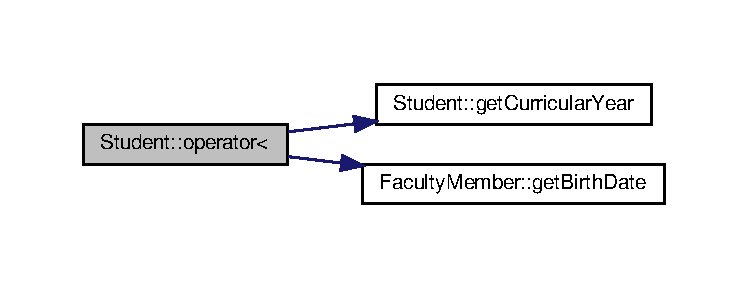
\includegraphics[width=350pt]{classStudent_aabc24d469d7206a621fa154b3578d9e0_cgraph}
\end{center}
\end{figure}
\mbox{\Hypertarget{classStudent_a3567f5c4220ffa88a8855998b3b99b43}\label{classStudent_a3567f5c4220ffa88a8855998b3b99b43}} 
\index{Student@{Student}!print\+Info@{print\+Info}}
\index{print\+Info@{print\+Info}!Student@{Student}}
\subsubsection{\texorpdfstring{print\+Info()}{printInfo()}}
{\footnotesize\ttfamily void Student\+::print\+Info (\begin{DoxyParamCaption}{ }\end{DoxyParamCaption}) const\hspace{0.3cm}{\ttfamily [virtual]}}

Prints the information of a student, that is, the value of every attribute of the object 

Reimplemented from \hyperlink{classFacultyMember_af07c814d58d1a2e309c74a0c57b95fd1}{Faculty\+Member}.



Definition at line 229 of file Faculty\+Member.\+cpp.

Here is the call graph for this function\+:\nopagebreak
\begin{figure}[H]
\begin{center}
\leavevmode
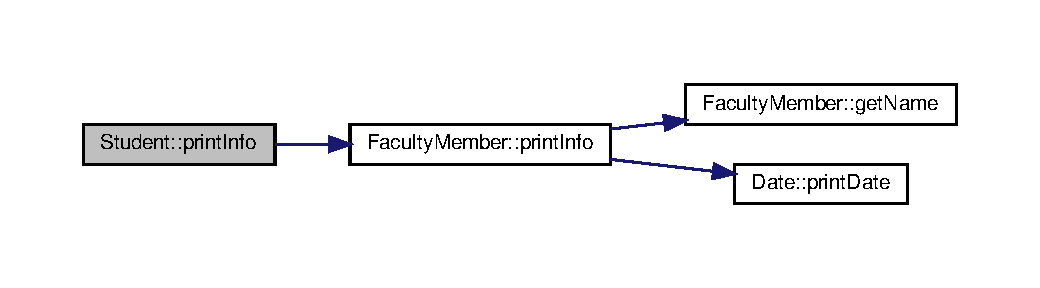
\includegraphics[width=350pt]{classStudent_a3567f5c4220ffa88a8855998b3b99b43_cgraph}
\end{center}
\end{figure}
\mbox{\Hypertarget{classStudent_a5b0b522fd636bfc266a08129a8784a0a}\label{classStudent_a5b0b522fd636bfc266a08129a8784a0a}} 
\index{Student@{Student}!set\+Average@{set\+Average}}
\index{set\+Average@{set\+Average}!Student@{Student}}
\subsubsection{\texorpdfstring{set\+Average()}{setAverage()}}
{\footnotesize\ttfamily void Student\+::set\+Average (\begin{DoxyParamCaption}\item[{float}]{average }\end{DoxyParamCaption})}



Sets the average of a student. 


\begin{DoxyParams}{Parameters}
{\em average} & The average of a student \\
\hline
\end{DoxyParams}


Definition at line 201 of file Faculty\+Member.\+cpp.

\mbox{\Hypertarget{classStudent_af7affdfd5b1b9e4d8c8d1fcb1e2cc631}\label{classStudent_af7affdfd5b1b9e4d8c8d1fcb1e2cc631}} 
\index{Student@{Student}!set\+Course@{set\+Course}}
\index{set\+Course@{set\+Course}!Student@{Student}}
\subsubsection{\texorpdfstring{set\+Course()}{setCourse()}}
{\footnotesize\ttfamily void Student\+::set\+Course (\begin{DoxyParamCaption}\item[{int}]{course }\end{DoxyParamCaption})}

Sets the course of a student 
\begin{DoxyParams}{Parameters}
{\em course} & The course \\
\hline
\end{DoxyParams}


Definition at line 247 of file Faculty\+Member.\+cpp.

\mbox{\Hypertarget{classStudent_a2a24ebdce323c9cea4060b1cd9d343c9}\label{classStudent_a2a24ebdce323c9cea4060b1cd9d343c9}} 
\index{Student@{Student}!set\+Subjects\+Taken@{set\+Subjects\+Taken}}
\index{set\+Subjects\+Taken@{set\+Subjects\+Taken}!Student@{Student}}
\subsubsection{\texorpdfstring{set\+Subjects\+Taken()}{setSubjectsTaken()}}
{\footnotesize\ttfamily void Student\+::set\+Subjects\+Taken (\begin{DoxyParamCaption}\item[{std\+::vector$<$ \hyperlink{classSubject}{Subject} $>$}]{subjects }\end{DoxyParamCaption})}

Sets the subjects taken by the student 
\begin{DoxyParams}{Parameters}
{\em subjects} & Subjects taken by the student \\
\hline
\end{DoxyParams}


Definition at line 264 of file Faculty\+Member.\+cpp.



The documentation for this class was generated from the following files\+:\begin{DoxyCompactItemize}
\item 
include/Faculty\+Member.\+hpp\item 
src/Faculty\+Member.\+cpp\end{DoxyCompactItemize}

\hypertarget{classStudentPtr}{}\section{Student\+Ptr Class Reference}
\label{classStudentPtr}\index{Student\+Ptr@{Student\+Ptr}}
\subsection*{Public Member Functions}
\begin{DoxyCompactItemize}
\item 
\mbox{\Hypertarget{classStudentPtr_a9e9b100f8bd5978b3eb07299d62d9202}\label{classStudentPtr_a9e9b100f8bd5978b3eb07299d62d9202}} 
{\bfseries Student\+Ptr} (\hyperlink{classStudent}{Student} $\ast$s)
\item 
\mbox{\Hypertarget{classStudentPtr_a6274fd86457eba16361c8bcf45cf1184}\label{classStudentPtr_a6274fd86457eba16361c8bcf45cf1184}} 
\hyperlink{classStudent}{Student} $\ast$ {\bfseries get\+Ptr} () const
\item 
\mbox{\Hypertarget{classStudentPtr_ab66466487798e421390290c0eae31757}\label{classStudentPtr_ab66466487798e421390290c0eae31757}} 
void {\bfseries print} () const
\item 
\mbox{\Hypertarget{classStudentPtr_ab2e10ac137df65b568bfc7b3bb800b53}\label{classStudentPtr_ab2e10ac137df65b568bfc7b3bb800b53}} 
bool {\bfseries operator$<$} (const \hyperlink{classStudentPtr}{Student\+Ptr} \&s1) const
\item 
\mbox{\Hypertarget{classStudentPtr_a0dcd1136bd074769f38f36f4931aace4}\label{classStudentPtr_a0dcd1136bd074769f38f36f4931aace4}} 
bool {\bfseries operator==} (const \hyperlink{classStudentPtr}{Student\+Ptr} \&s1) const
\end{DoxyCompactItemize}


\subsection{Detailed Description}


Definition at line 116 of file Faculty\+Member.\+hpp.



The documentation for this class was generated from the following files\+:\begin{DoxyCompactItemize}
\item 
include/Faculty\+Member.\+hpp\item 
src/Faculty\+Member.\+cpp\end{DoxyCompactItemize}

\hypertarget{classSubject}{}\section{Subject Class Reference}
\label{classSubject}\index{Subject@{Subject}}
\subsection*{Public Member Functions}
\begin{DoxyCompactItemize}
\item 
\hyperlink{classSubject_a6fd4f94feaeb80fb410278015b38ad94}{Subject} (std\+::string name\+PT, std\+::string name\+EN, int regent\+Code, int code, int lective\+Year, float E\+C\+TS, int work\+Load)
\item 
bool \hyperlink{classSubject_a2ba88df904eeb87b136764898ea3a1fc}{operator$<$} (const \hyperlink{classSubject}{Subject} c) const
\item 
bool \hyperlink{classSubject_acc7e7e8b0665e05dd9f0d78a6d79468f}{operator==} (const \hyperlink{classSubject}{Subject} C) const
\item 
std\+::string \hyperlink{classSubject_a4fb200b5b33dab2166a9a1ee6dbe7443}{get\+Name\+PT} () const
\item 
std\+::string \hyperlink{classSubject_a9419a1c4e2248fee00baf3885655ba49}{get\+Name\+EN} () const
\item 
int \hyperlink{classSubject_afbdb9379e3d0ceb44b838cf113931a23}{get\+Regent\+Code} () const
\item 
int \hyperlink{classSubject_a2d962550a5b15b5cdf3eb0d8892957f8}{get\+Code} () const
\item 
int \hyperlink{classSubject_ad03c422fb716222b2c49c41b7506827a}{get\+Lective\+Year} () const
\item 
float \hyperlink{classSubject_a1395a7f637471df28cc72b8b746350d1}{get\+E\+C\+TS} () const
\item 
int \hyperlink{classSubject_a628fc24fd443deb1ab62e4dc05e8ec25}{get\+Work\+Load} () const
\item 
std\+::vector$<$ int $>$ \hyperlink{classSubject_ab82fbd086ac1f72b52fbaa2143558eeb}{get\+Teachers\+Code} () const
\item 
std\+::vector$<$ int $>$ \hyperlink{classSubject_a668e1cc5e5b0a6422d58134fae5aae7e}{get\+Students\+Code} () const
\item 
std\+::map$<$ int, float $>$ \hyperlink{classSubject_ac9837d37f7d4e94759622e736a5b4ff9}{get\+Grades} () const
\item 
float \hyperlink{classSubject_a625235d561cd4266a23cc6a09fddadc8}{get\+Student\+Grade} (int student\+Code) const
\item 
void \hyperlink{classSubject_ae0571c4d3b1b46c48dc4bc540d450294}{insert\+Grade} (int student\+ID, float grade)
\item 
void \hyperlink{classSubject_af96ca779862097e5cc1bb2b457ba08a2}{print\+Info} () const
\item 
void \hyperlink{classSubject_afbae90dc81a1ceb1f5ccf0099639e265}{set\+Name\+PT} (std\+::string name)
\item 
void \hyperlink{classSubject_af9e9958808eccfa4afaf702f560b0e6d}{set\+Name\+EN} (std\+::string name)
\item 
void \hyperlink{classSubject_a6d2cf53e66fdb1ac6658c03d5be73b3e}{set\+Regent\+Code} (int code)
\item 
void \hyperlink{classSubject_aecdbb1db33e14fd380bcb607a33c86e8}{set\+Code} (int code)
\item 
void \hyperlink{classSubject_acf269c84f61028d400856b94677e6422}{set\+Lective\+Year} (int lective\+Year)
\item 
void \hyperlink{classSubject_ab2b31d04366a75b679f1eec77783e0bf}{set\+E\+C\+TS} (float E\+C\+TS)
\item 
void \hyperlink{classSubject_aafa4294e098c5c1257a8b5ba75ff1cb6}{set\+Work\+Load} (int work\+Load)
\item 
void \hyperlink{classSubject_af4e5480d466cd44214dd006bec2f891a}{set\+Grades} (std\+::map$<$ int, float $>$ map)
\item 
void \hyperlink{classSubject_a1799fa0aaa5f81dd370bab999be15c43}{add\+Teachers\+Code} (int code)
\item 
void \hyperlink{classSubject_afa7d78b9fed5b72cfebf3d19fe03d22f}{add\+Students\+Code} (int code)
\item 
\mbox{\Hypertarget{classSubject_a5d9a4918eeb1e276ca0d43427bb5ce82}\label{classSubject_a5d9a4918eeb1e276ca0d43427bb5ce82}} 
void {\bfseries compated\+Information} (std\+::ofstream \&f)
\item 
\mbox{\Hypertarget{classSubject_a87390cb731f0c7c2c083ee202fcb4262}\label{classSubject_a87390cb731f0c7c2c083ee202fcb4262}} 
void {\bfseries set\+Teachers\+Code} (vector$<$ int $>$ codes)
\item 
\mbox{\Hypertarget{classSubject_a4e033c353b3c1b2c670a29233854872d}\label{classSubject_a4e033c353b3c1b2c670a29233854872d}} 
void {\bfseries set\+Students\+Code} (vector$<$ int $>$ codes)
\end{DoxyCompactItemize}
\subsection*{Protected Attributes}
\begin{DoxyCompactItemize}
\item 
\mbox{\Hypertarget{classSubject_a6a737e1a646acda7d16f0f4d62dbd6e1}\label{classSubject_a6a737e1a646acda7d16f0f4d62dbd6e1}} 
std\+::string {\bfseries name\+PT}
\item 
\mbox{\Hypertarget{classSubject_aa78ad6c245d0adb04661d754f545bf7f}\label{classSubject_aa78ad6c245d0adb04661d754f545bf7f}} 
std\+::string {\bfseries name\+EN}
\item 
\mbox{\Hypertarget{classSubject_a7fc044615a85c88d8a09b19aa782f4fa}\label{classSubject_a7fc044615a85c88d8a09b19aa782f4fa}} 
int {\bfseries regent\+Code}
\item 
\mbox{\Hypertarget{classSubject_a69b906cc97243b4c6def833f2de8115f}\label{classSubject_a69b906cc97243b4c6def833f2de8115f}} 
int {\bfseries code}
\item 
\mbox{\Hypertarget{classSubject_ac47c5327d56f61d8ec5acb7040775d3f}\label{classSubject_ac47c5327d56f61d8ec5acb7040775d3f}} 
int {\bfseries lective\+Year}
\item 
\mbox{\Hypertarget{classSubject_aeb65ed41d5e97b96528d10e9166d85f5}\label{classSubject_aeb65ed41d5e97b96528d10e9166d85f5}} 
float {\bfseries E\+C\+TS}
\item 
\mbox{\Hypertarget{classSubject_a868584632f241bbba39f7adc35dc276f}\label{classSubject_a868584632f241bbba39f7adc35dc276f}} 
int {\bfseries work\+Load}
\item 
\mbox{\Hypertarget{classSubject_a5d16b700a6d4e2d93bcbf1fdd2c5c08c}\label{classSubject_a5d16b700a6d4e2d93bcbf1fdd2c5c08c}} 
std\+::vector$<$ int $>$ {\bfseries teachers\+Code}
\item 
\mbox{\Hypertarget{classSubject_a3b5cc22b3be0be611a2626a705882fa5}\label{classSubject_a3b5cc22b3be0be611a2626a705882fa5}} 
std\+::vector$<$ int $>$ {\bfseries students\+Code}
\item 
\mbox{\Hypertarget{classSubject_a708b21c280618eac769d1711bac4749e}\label{classSubject_a708b21c280618eac769d1711bac4749e}} 
std\+::map$<$ int, float $>$ {\bfseries grades}
\end{DoxyCompactItemize}


\subsection{Detailed Description}


Definition at line 13 of file Subject.\+hpp.



\subsection{Constructor \& Destructor Documentation}
\mbox{\Hypertarget{classSubject_a6fd4f94feaeb80fb410278015b38ad94}\label{classSubject_a6fd4f94feaeb80fb410278015b38ad94}} 
\index{Subject@{Subject}!Subject@{Subject}}
\index{Subject@{Subject}!Subject@{Subject}}
\subsubsection{\texorpdfstring{Subject()}{Subject()}}
{\footnotesize\ttfamily Subject\+::\+Subject (\begin{DoxyParamCaption}\item[{std\+::string}]{name\+PT,  }\item[{std\+::string}]{name\+EN,  }\item[{int}]{regent\+Code,  }\item[{int}]{code,  }\item[{int}]{lective\+Year,  }\item[{float}]{E\+C\+TS,  }\item[{int}]{work\+Load }\end{DoxyParamCaption})}

Constructs a subject with all the attribute values as parameter values 
\begin{DoxyParams}{Parameters}
{\em name\+PT} & The portuguese name of the subject \\
\hline
{\em name\+EN} & The english name of the subject \\
\hline
{\em regent\+Code} & The regent code of the subject \\
\hline
{\em code} & The code of the subject \\
\hline
{\em lective\+Year} & The lective year of the subject \\
\hline
{\em E\+C\+TS} & The E\+C\+T\+Ss of the subject \\
\hline
{\em work\+Load} & The workload of the subject \\
\hline
{\em teachers\+Code} & The codes of the teachers that teach the subject \\
\hline
{\em students\+Code} & The codes of the students that are enrolled in the subject \\
\hline
\end{DoxyParams}


Definition at line 16 of file Subject.\+cpp.



\subsection{Member Function Documentation}
\mbox{\Hypertarget{classSubject_afa7d78b9fed5b72cfebf3d19fe03d22f}\label{classSubject_afa7d78b9fed5b72cfebf3d19fe03d22f}} 
\index{Subject@{Subject}!add\+Students\+Code@{add\+Students\+Code}}
\index{add\+Students\+Code@{add\+Students\+Code}!Subject@{Subject}}
\subsubsection{\texorpdfstring{add\+Students\+Code()}{addStudentsCode()}}
{\footnotesize\ttfamily void Subject\+::add\+Students\+Code (\begin{DoxyParamCaption}\item[{int}]{code }\end{DoxyParamCaption})}

Adds the code of a student to the vector of students that teach the subject 
\begin{DoxyParams}{Parameters}
{\em code} & The code of the student \\
\hline
\end{DoxyParams}


Definition at line 320 of file Subject.\+cpp.

\mbox{\Hypertarget{classSubject_a1799fa0aaa5f81dd370bab999be15c43}\label{classSubject_a1799fa0aaa5f81dd370bab999be15c43}} 
\index{Subject@{Subject}!add\+Teachers\+Code@{add\+Teachers\+Code}}
\index{add\+Teachers\+Code@{add\+Teachers\+Code}!Subject@{Subject}}
\subsubsection{\texorpdfstring{add\+Teachers\+Code()}{addTeachersCode()}}
{\footnotesize\ttfamily void Subject\+::add\+Teachers\+Code (\begin{DoxyParamCaption}\item[{int}]{code }\end{DoxyParamCaption})}

Adds the code of a teacher to the vector of teachers that teach the subject 
\begin{DoxyParams}{Parameters}
{\em code} & The code of the teacher \\
\hline
\end{DoxyParams}


Definition at line 310 of file Subject.\+cpp.

\mbox{\Hypertarget{classSubject_a2d962550a5b15b5cdf3eb0d8892957f8}\label{classSubject_a2d962550a5b15b5cdf3eb0d8892957f8}} 
\index{Subject@{Subject}!get\+Code@{get\+Code}}
\index{get\+Code@{get\+Code}!Subject@{Subject}}
\subsubsection{\texorpdfstring{get\+Code()}{getCode()}}
{\footnotesize\ttfamily int Subject\+::get\+Code (\begin{DoxyParamCaption}{ }\end{DoxyParamCaption}) const}

Returns the code of the subject \begin{DoxyReturn}{Returns}

\end{DoxyReturn}


Definition at line 131 of file Subject.\+cpp.

\mbox{\Hypertarget{classSubject_a1395a7f637471df28cc72b8b746350d1}\label{classSubject_a1395a7f637471df28cc72b8b746350d1}} 
\index{Subject@{Subject}!get\+E\+C\+TS@{get\+E\+C\+TS}}
\index{get\+E\+C\+TS@{get\+E\+C\+TS}!Subject@{Subject}}
\subsubsection{\texorpdfstring{get\+E\+C\+T\+S()}{getECTS()}}
{\footnotesize\ttfamily float Subject\+::get\+E\+C\+TS (\begin{DoxyParamCaption}{ }\end{DoxyParamCaption}) const}

Returns the E\+C\+T\+Ss of the subject \begin{DoxyReturn}{Returns}
The E\+C\+T\+Ss of the subject 
\end{DoxyReturn}


Definition at line 149 of file Subject.\+cpp.

\mbox{\Hypertarget{classSubject_ac9837d37f7d4e94759622e736a5b4ff9}\label{classSubject_ac9837d37f7d4e94759622e736a5b4ff9}} 
\index{Subject@{Subject}!get\+Grades@{get\+Grades}}
\index{get\+Grades@{get\+Grades}!Subject@{Subject}}
\subsubsection{\texorpdfstring{get\+Grades()}{getGrades()}}
{\footnotesize\ttfamily std\+::map$<$ int, float $>$ Subject\+::get\+Grades (\begin{DoxyParamCaption}{ }\end{DoxyParamCaption}) const}

Gets the grades of a given student, in which the first member of the map is the code of the student, and the second member of the map is the grade of the student in this subject \begin{DoxyReturn}{Returns}

\end{DoxyReturn}


Definition at line 170 of file Subject.\+cpp.

\mbox{\Hypertarget{classSubject_ad03c422fb716222b2c49c41b7506827a}\label{classSubject_ad03c422fb716222b2c49c41b7506827a}} 
\index{Subject@{Subject}!get\+Lective\+Year@{get\+Lective\+Year}}
\index{get\+Lective\+Year@{get\+Lective\+Year}!Subject@{Subject}}
\subsubsection{\texorpdfstring{get\+Lective\+Year()}{getLectiveYear()}}
{\footnotesize\ttfamily int Subject\+::get\+Lective\+Year (\begin{DoxyParamCaption}{ }\end{DoxyParamCaption}) const}

Returns the lective year of the subject \begin{DoxyReturn}{Returns}

\end{DoxyReturn}


Definition at line 140 of file Subject.\+cpp.

\mbox{\Hypertarget{classSubject_a9419a1c4e2248fee00baf3885655ba49}\label{classSubject_a9419a1c4e2248fee00baf3885655ba49}} 
\index{Subject@{Subject}!get\+Name\+EN@{get\+Name\+EN}}
\index{get\+Name\+EN@{get\+Name\+EN}!Subject@{Subject}}
\subsubsection{\texorpdfstring{get\+Name\+E\+N()}{getNameEN()}}
{\footnotesize\ttfamily std\+::string Subject\+::get\+Name\+EN (\begin{DoxyParamCaption}{ }\end{DoxyParamCaption}) const}

Gets the english name of the subject \begin{DoxyReturn}{Returns}
The english name of the subjest 
\end{DoxyReturn}


Definition at line 86 of file Subject.\+cpp.

\mbox{\Hypertarget{classSubject_a4fb200b5b33dab2166a9a1ee6dbe7443}\label{classSubject_a4fb200b5b33dab2166a9a1ee6dbe7443}} 
\index{Subject@{Subject}!get\+Name\+PT@{get\+Name\+PT}}
\index{get\+Name\+PT@{get\+Name\+PT}!Subject@{Subject}}
\subsubsection{\texorpdfstring{get\+Name\+P\+T()}{getNamePT()}}
{\footnotesize\ttfamily std\+::string Subject\+::get\+Name\+PT (\begin{DoxyParamCaption}{ }\end{DoxyParamCaption}) const}

Gets the portuguese name of the subject \begin{DoxyReturn}{Returns}
The portuguese name of the subject 
\end{DoxyReturn}


Definition at line 77 of file Subject.\+cpp.

\mbox{\Hypertarget{classSubject_afbdb9379e3d0ceb44b838cf113931a23}\label{classSubject_afbdb9379e3d0ceb44b838cf113931a23}} 
\index{Subject@{Subject}!get\+Regent\+Code@{get\+Regent\+Code}}
\index{get\+Regent\+Code@{get\+Regent\+Code}!Subject@{Subject}}
\subsubsection{\texorpdfstring{get\+Regent\+Code()}{getRegentCode()}}
{\footnotesize\ttfamily int Subject\+::get\+Regent\+Code (\begin{DoxyParamCaption}{ }\end{DoxyParamCaption}) const}

Gets the code of the regent of the subject \begin{DoxyReturn}{Returns}
The code of the regent of the subject 
\end{DoxyReturn}


Definition at line 95 of file Subject.\+cpp.

\mbox{\Hypertarget{classSubject_a625235d561cd4266a23cc6a09fddadc8}\label{classSubject_a625235d561cd4266a23cc6a09fddadc8}} 
\index{Subject@{Subject}!get\+Student\+Grade@{get\+Student\+Grade}}
\index{get\+Student\+Grade@{get\+Student\+Grade}!Subject@{Subject}}
\subsubsection{\texorpdfstring{get\+Student\+Grade()}{getStudentGrade()}}
{\footnotesize\ttfamily float Subject\+::get\+Student\+Grade (\begin{DoxyParamCaption}\item[{int}]{student\+Code }\end{DoxyParamCaption}) const}

Gets the grade of a student in the subject 
\begin{DoxyParams}{Parameters}
{\em student\+Code} & The code of the student \\
\hline
\end{DoxyParams}
\begin{DoxyReturn}{Returns}
The grade of the subject 
\end{DoxyReturn}


Definition at line 180 of file Subject.\+cpp.

\mbox{\Hypertarget{classSubject_a668e1cc5e5b0a6422d58134fae5aae7e}\label{classSubject_a668e1cc5e5b0a6422d58134fae5aae7e}} 
\index{Subject@{Subject}!get\+Students\+Code@{get\+Students\+Code}}
\index{get\+Students\+Code@{get\+Students\+Code}!Subject@{Subject}}
\subsubsection{\texorpdfstring{get\+Students\+Code()}{getStudentsCode()}}
{\footnotesize\ttfamily std\+::vector$<$ int $>$ Subject\+::get\+Students\+Code (\begin{DoxyParamCaption}{ }\end{DoxyParamCaption}) const}

Gets the codes of every student that is enrolled in the subject \begin{DoxyReturn}{Returns}
The codes of every student enrolled in the subject 
\end{DoxyReturn}


Definition at line 68 of file Subject.\+cpp.

\mbox{\Hypertarget{classSubject_ab82fbd086ac1f72b52fbaa2143558eeb}\label{classSubject_ab82fbd086ac1f72b52fbaa2143558eeb}} 
\index{Subject@{Subject}!get\+Teachers\+Code@{get\+Teachers\+Code}}
\index{get\+Teachers\+Code@{get\+Teachers\+Code}!Subject@{Subject}}
\subsubsection{\texorpdfstring{get\+Teachers\+Code()}{getTeachersCode()}}
{\footnotesize\ttfamily std\+::vector$<$ int $>$ Subject\+::get\+Teachers\+Code (\begin{DoxyParamCaption}{ }\end{DoxyParamCaption}) const}

Gets the codes of every teacher that teaches the subject \begin{DoxyReturn}{Returns}
The codes of the teachers that teach the subject 
\end{DoxyReturn}


Definition at line 58 of file Subject.\+cpp.

\mbox{\Hypertarget{classSubject_a628fc24fd443deb1ab62e4dc05e8ec25}\label{classSubject_a628fc24fd443deb1ab62e4dc05e8ec25}} 
\index{Subject@{Subject}!get\+Work\+Load@{get\+Work\+Load}}
\index{get\+Work\+Load@{get\+Work\+Load}!Subject@{Subject}}
\subsubsection{\texorpdfstring{get\+Work\+Load()}{getWorkLoad()}}
{\footnotesize\ttfamily int Subject\+::get\+Work\+Load (\begin{DoxyParamCaption}{ }\end{DoxyParamCaption}) const}

Gets the work load of the subject \begin{DoxyReturn}{Returns}
The work load of the subject 
\end{DoxyReturn}


Definition at line 158 of file Subject.\+cpp.

\mbox{\Hypertarget{classSubject_ae0571c4d3b1b46c48dc4bc540d450294}\label{classSubject_ae0571c4d3b1b46c48dc4bc540d450294}} 
\index{Subject@{Subject}!insert\+Grade@{insert\+Grade}}
\index{insert\+Grade@{insert\+Grade}!Subject@{Subject}}
\subsubsection{\texorpdfstring{insert\+Grade()}{insertGrade()}}
{\footnotesize\ttfamily void Subject\+::insert\+Grade (\begin{DoxyParamCaption}\item[{int}]{studend\+ID,  }\item[{float}]{grade }\end{DoxyParamCaption})}

Inserts the grade of a student 
\begin{DoxyParams}{Parameters}
{\em studend\+ID} & The code of the student \\
\hline
{\em grade} & The grade of the student \\
\hline
\end{DoxyParams}


Definition at line 192 of file Subject.\+cpp.

\mbox{\Hypertarget{classSubject_a2ba88df904eeb87b136764898ea3a1fc}\label{classSubject_a2ba88df904eeb87b136764898ea3a1fc}} 
\index{Subject@{Subject}!operator$<$@{operator$<$}}
\index{operator$<$@{operator$<$}!Subject@{Subject}}
\subsubsection{\texorpdfstring{operator$<$()}{operator<()}}
{\footnotesize\ttfamily bool Subject\+::operator$<$ (\begin{DoxyParamCaption}\item[{const \hyperlink{classSubject}{Subject}}]{C }\end{DoxyParamCaption}) const}

Gets the smallest subject of the two subjects provided 
\begin{DoxyParams}{Parameters}
{\em C} & A subject to be compared \\
\hline
\end{DoxyParams}
\begin{DoxyReturn}{Returns}
The smallest subject 
\end{DoxyReturn}


Definition at line 106 of file Subject.\+cpp.

Here is the call graph for this function\+:\nopagebreak
\begin{figure}[H]
\begin{center}
\leavevmode
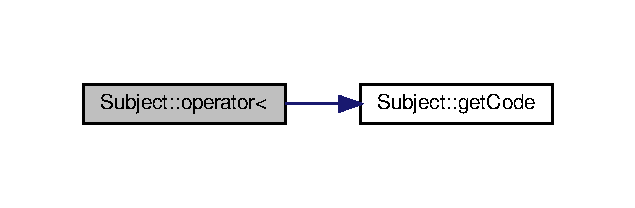
\includegraphics[width=305pt]{classSubject_a2ba88df904eeb87b136764898ea3a1fc_cgraph}
\end{center}
\end{figure}
\mbox{\Hypertarget{classSubject_acc7e7e8b0665e05dd9f0d78a6d79468f}\label{classSubject_acc7e7e8b0665e05dd9f0d78a6d79468f}} 
\index{Subject@{Subject}!operator==@{operator==}}
\index{operator==@{operator==}!Subject@{Subject}}
\subsubsection{\texorpdfstring{operator==()}{operator==()}}
{\footnotesize\ttfamily bool Subject\+::operator== (\begin{DoxyParamCaption}\item[{const \hyperlink{classSubject}{Subject}}]{c }\end{DoxyParamCaption}) const}

Tells if two subjects are equal 
\begin{DoxyParams}{Parameters}
{\em c} & A subject to be compared \\
\hline
\end{DoxyParams}
\begin{DoxyReturn}{Returns}
The result of the operation 
\end{DoxyReturn}


Definition at line 116 of file Subject.\+cpp.

\mbox{\Hypertarget{classSubject_af96ca779862097e5cc1bb2b457ba08a2}\label{classSubject_af96ca779862097e5cc1bb2b457ba08a2}} 
\index{Subject@{Subject}!print\+Info@{print\+Info}}
\index{print\+Info@{print\+Info}!Subject@{Subject}}
\subsubsection{\texorpdfstring{print\+Info()}{printInfo()}}
{\footnotesize\ttfamily void Subject\+::print\+Info (\begin{DoxyParamCaption}{ }\end{DoxyParamCaption}) const}

Prints the info of the subject, that is, the value of all its attributes 

Definition at line 201 of file Subject.\+cpp.

\mbox{\Hypertarget{classSubject_aecdbb1db33e14fd380bcb607a33c86e8}\label{classSubject_aecdbb1db33e14fd380bcb607a33c86e8}} 
\index{Subject@{Subject}!set\+Code@{set\+Code}}
\index{set\+Code@{set\+Code}!Subject@{Subject}}
\subsubsection{\texorpdfstring{set\+Code()}{setCode()}}
{\footnotesize\ttfamily void Subject\+::set\+Code (\begin{DoxyParamCaption}\item[{int}]{code }\end{DoxyParamCaption})}

Sets the code of the subject 
\begin{DoxyParams}{Parameters}
{\em code} & The code of the subject \\
\hline
\end{DoxyParams}


Definition at line 273 of file Subject.\+cpp.

\mbox{\Hypertarget{classSubject_ab2b31d04366a75b679f1eec77783e0bf}\label{classSubject_ab2b31d04366a75b679f1eec77783e0bf}} 
\index{Subject@{Subject}!set\+E\+C\+TS@{set\+E\+C\+TS}}
\index{set\+E\+C\+TS@{set\+E\+C\+TS}!Subject@{Subject}}
\subsubsection{\texorpdfstring{set\+E\+C\+T\+S()}{setECTS()}}
{\footnotesize\ttfamily void Subject\+::set\+E\+C\+TS (\begin{DoxyParamCaption}\item[{float}]{E\+C\+TS }\end{DoxyParamCaption})}

Sets the E\+C\+T\+Ss of the subject 
\begin{DoxyParams}{Parameters}
{\em E\+C\+TS} & The E\+C\+T\+Ss \\
\hline
\end{DoxyParams}


Definition at line 291 of file Subject.\+cpp.

\mbox{\Hypertarget{classSubject_af4e5480d466cd44214dd006bec2f891a}\label{classSubject_af4e5480d466cd44214dd006bec2f891a}} 
\index{Subject@{Subject}!set\+Grades@{set\+Grades}}
\index{set\+Grades@{set\+Grades}!Subject@{Subject}}
\subsubsection{\texorpdfstring{set\+Grades()}{setGrades()}}
{\footnotesize\ttfamily void Subject\+::set\+Grades (\begin{DoxyParamCaption}\item[{std\+::map$<$ int, float $>$}]{grades }\end{DoxyParamCaption})}

Sets the grades of every student 
\begin{DoxyParams}{Parameters}
{\em grades} & The grades of every student \\
\hline
\end{DoxyParams}


Definition at line 329 of file Subject.\+cpp.

\mbox{\Hypertarget{classSubject_acf269c84f61028d400856b94677e6422}\label{classSubject_acf269c84f61028d400856b94677e6422}} 
\index{Subject@{Subject}!set\+Lective\+Year@{set\+Lective\+Year}}
\index{set\+Lective\+Year@{set\+Lective\+Year}!Subject@{Subject}}
\subsubsection{\texorpdfstring{set\+Lective\+Year()}{setLectiveYear()}}
{\footnotesize\ttfamily void Subject\+::set\+Lective\+Year (\begin{DoxyParamCaption}\item[{int}]{lective\+Year }\end{DoxyParamCaption})}

Sets the lective year of the subject 
\begin{DoxyParams}{Parameters}
{\em lective\+Year} & The lective year \\
\hline
\end{DoxyParams}


Definition at line 282 of file Subject.\+cpp.

\mbox{\Hypertarget{classSubject_af9e9958808eccfa4afaf702f560b0e6d}\label{classSubject_af9e9958808eccfa4afaf702f560b0e6d}} 
\index{Subject@{Subject}!set\+Name\+EN@{set\+Name\+EN}}
\index{set\+Name\+EN@{set\+Name\+EN}!Subject@{Subject}}
\subsubsection{\texorpdfstring{set\+Name\+E\+N()}{setNameEN()}}
{\footnotesize\ttfamily void Subject\+::set\+Name\+EN (\begin{DoxyParamCaption}\item[{std\+::string}]{name }\end{DoxyParamCaption})}

Sets the english name of the subject 
\begin{DoxyParams}{Parameters}
{\em name} & The english name of the subject \\
\hline
\end{DoxyParams}


Definition at line 255 of file Subject.\+cpp.

\mbox{\Hypertarget{classSubject_afbae90dc81a1ceb1f5ccf0099639e265}\label{classSubject_afbae90dc81a1ceb1f5ccf0099639e265}} 
\index{Subject@{Subject}!set\+Name\+PT@{set\+Name\+PT}}
\index{set\+Name\+PT@{set\+Name\+PT}!Subject@{Subject}}
\subsubsection{\texorpdfstring{set\+Name\+P\+T()}{setNamePT()}}
{\footnotesize\ttfamily void Subject\+::set\+Name\+PT (\begin{DoxyParamCaption}\item[{std\+::string}]{name }\end{DoxyParamCaption})}

Sets the portuguese name of the subject 
\begin{DoxyParams}{Parameters}
{\em name} & The name of the subject \\
\hline
\end{DoxyParams}


Definition at line 246 of file Subject.\+cpp.

\mbox{\Hypertarget{classSubject_a6d2cf53e66fdb1ac6658c03d5be73b3e}\label{classSubject_a6d2cf53e66fdb1ac6658c03d5be73b3e}} 
\index{Subject@{Subject}!set\+Regent\+Code@{set\+Regent\+Code}}
\index{set\+Regent\+Code@{set\+Regent\+Code}!Subject@{Subject}}
\subsubsection{\texorpdfstring{set\+Regent\+Code()}{setRegentCode()}}
{\footnotesize\ttfamily void Subject\+::set\+Regent\+Code (\begin{DoxyParamCaption}\item[{int}]{code }\end{DoxyParamCaption})}

Sets the regent code of the subject 
\begin{DoxyParams}{Parameters}
{\em code} & Code of the regent \\
\hline
\end{DoxyParams}


Definition at line 264 of file Subject.\+cpp.

\mbox{\Hypertarget{classSubject_aafa4294e098c5c1257a8b5ba75ff1cb6}\label{classSubject_aafa4294e098c5c1257a8b5ba75ff1cb6}} 
\index{Subject@{Subject}!set\+Work\+Load@{set\+Work\+Load}}
\index{set\+Work\+Load@{set\+Work\+Load}!Subject@{Subject}}
\subsubsection{\texorpdfstring{set\+Work\+Load()}{setWorkLoad()}}
{\footnotesize\ttfamily void Subject\+::set\+Work\+Load (\begin{DoxyParamCaption}\item[{int}]{work\+Load }\end{DoxyParamCaption})}

Sets the work load of the subject 
\begin{DoxyParams}{Parameters}
{\em work\+Load} & The work load \\
\hline
\end{DoxyParams}


Definition at line 300 of file Subject.\+cpp.



The documentation for this class was generated from the following files\+:\begin{DoxyCompactItemize}
\item 
include/Subject.\+hpp\item 
src/Subject.\+cpp\end{DoxyCompactItemize}

\hypertarget{classTeacher}{}\section{Teacher Class Reference}
\label{classTeacher}\index{Teacher@{Teacher}}


Inheritance diagram for Teacher\+:\nopagebreak
\begin{figure}[H]
\begin{center}
\leavevmode
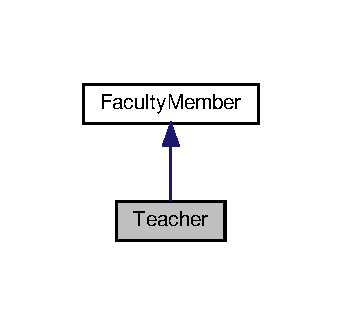
\includegraphics[width=164pt]{classTeacher__inherit__graph}
\end{center}
\end{figure}


Collaboration diagram for Teacher\+:\nopagebreak
\begin{figure}[H]
\begin{center}
\leavevmode
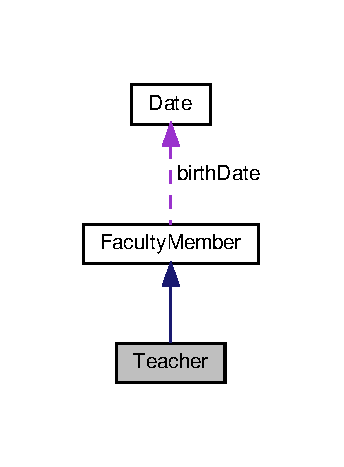
\includegraphics[width=165pt]{classTeacher__coll__graph}
\end{center}
\end{figure}
\subsection*{Public Member Functions}
\begin{DoxyCompactItemize}
\item 
\mbox{\Hypertarget{classTeacher_a844ddfba3aa130fddb487a862b5b7dab}\label{classTeacher_a844ddfba3aa130fddb487a862b5b7dab}} 
{\bfseries Teacher} (std\+::string name, std\+::string address, \hyperlink{classDate}{Date} birth\+Date, int cellphone\+Number, int code, int tax\+Payer\+Number, int salary, string category)
\item 
int \hyperlink{classTeacher_a3799bff1314b56a805273da1166304a3}{get\+Taxpayer\+Number} () const
\item 
int \hyperlink{classTeacher_abd551fc16a882af2eaaaade03dfc4dc9}{get\+Salary} () const
\item 
void \hyperlink{classTeacher_ae1fc6d174a25c714bfb73abf4620de03}{print\+Info} () const
\item 
void \hyperlink{classTeacher_a76e9731a32474291c679de1b7c8ddad5}{set\+Taxpayer\+Number} (int number)
\item 
void \hyperlink{classTeacher_a3d87b4630b21c0d7a8aa4651593a0937}{set\+Salary} (int salary)
\item 
void \hyperlink{classTeacher_ab713b38d67cafbe0d1c51eb73921e1a7}{set\+Category} (std\+::string category)
\item 
void \hyperlink{classTeacher_aac2aba678e32ce5a5f57989b55dc0952}{set\+Subjects} (std\+::vector$<$ \hyperlink{classSubject}{Subject} $>$ subjects)
\item 
\mbox{\Hypertarget{classTeacher_a3fa54467f61048678701e6673e5e1c96}\label{classTeacher_a3fa54467f61048678701e6673e5e1c96}} 
void {\bfseries compated\+Information} (std\+::ofstream \&f)
\end{DoxyCompactItemize}
\subsection*{Additional Inherited Members}


\subsection{Detailed Description}


Definition at line 71 of file Faculty\+Member.\+hpp.



\subsection{Member Function Documentation}
\mbox{\Hypertarget{classTeacher_abd551fc16a882af2eaaaade03dfc4dc9}\label{classTeacher_abd551fc16a882af2eaaaade03dfc4dc9}} 
\index{Teacher@{Teacher}!get\+Salary@{get\+Salary}}
\index{get\+Salary@{get\+Salary}!Teacher@{Teacher}}
\subsubsection{\texorpdfstring{get\+Salary()}{getSalary()}}
{\footnotesize\ttfamily int Teacher\+::get\+Salary (\begin{DoxyParamCaption}{ }\end{DoxyParamCaption}) const}

Gets the salary of a teacher \begin{DoxyReturn}{Returns}
The salary of the teacher 
\end{DoxyReturn}


Definition at line 355 of file Faculty\+Member.\+cpp.

\mbox{\Hypertarget{classTeacher_a3799bff1314b56a805273da1166304a3}\label{classTeacher_a3799bff1314b56a805273da1166304a3}} 
\index{Teacher@{Teacher}!get\+Taxpayer\+Number@{get\+Taxpayer\+Number}}
\index{get\+Taxpayer\+Number@{get\+Taxpayer\+Number}!Teacher@{Teacher}}
\subsubsection{\texorpdfstring{get\+Taxpayer\+Number()}{getTaxpayerNumber()}}
{\footnotesize\ttfamily int Teacher\+::get\+Taxpayer\+Number (\begin{DoxyParamCaption}{ }\end{DoxyParamCaption}) const}

Gets the taxpayer number of a teacher \begin{DoxyReturn}{Returns}
the taxpayer number of the teacher 
\end{DoxyReturn}


Definition at line 346 of file Faculty\+Member.\+cpp.

\mbox{\Hypertarget{classTeacher_ae1fc6d174a25c714bfb73abf4620de03}\label{classTeacher_ae1fc6d174a25c714bfb73abf4620de03}} 
\index{Teacher@{Teacher}!print\+Info@{print\+Info}}
\index{print\+Info@{print\+Info}!Teacher@{Teacher}}
\subsubsection{\texorpdfstring{print\+Info()}{printInfo()}}
{\footnotesize\ttfamily void Teacher\+::print\+Info (\begin{DoxyParamCaption}{ }\end{DoxyParamCaption}) const\hspace{0.3cm}{\ttfamily [virtual]}}

Prints the information of the teacher, that is, the value of every attribute of the object 

Reimplemented from \hyperlink{classFacultyMember_af07c814d58d1a2e309c74a0c57b95fd1}{Faculty\+Member}.



Definition at line 365 of file Faculty\+Member.\+cpp.

Here is the call graph for this function\+:\nopagebreak
\begin{figure}[H]
\begin{center}
\leavevmode
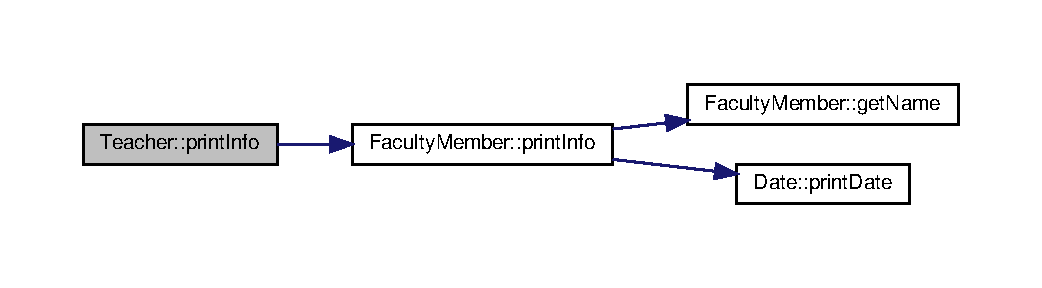
\includegraphics[width=350pt]{classTeacher_ae1fc6d174a25c714bfb73abf4620de03_cgraph}
\end{center}
\end{figure}
\mbox{\Hypertarget{classTeacher_ab713b38d67cafbe0d1c51eb73921e1a7}\label{classTeacher_ab713b38d67cafbe0d1c51eb73921e1a7}} 
\index{Teacher@{Teacher}!set\+Category@{set\+Category}}
\index{set\+Category@{set\+Category}!Teacher@{Teacher}}
\subsubsection{\texorpdfstring{set\+Category()}{setCategory()}}
{\footnotesize\ttfamily void Teacher\+::set\+Category (\begin{DoxyParamCaption}\item[{std\+::string}]{category }\end{DoxyParamCaption})}

Sets the category of the teacher 
\begin{DoxyParams}{Parameters}
{\em category} & The category of the teacher \\
\hline
\end{DoxyParams}


Definition at line 402 of file Faculty\+Member.\+cpp.

\mbox{\Hypertarget{classTeacher_a3d87b4630b21c0d7a8aa4651593a0937}\label{classTeacher_a3d87b4630b21c0d7a8aa4651593a0937}} 
\index{Teacher@{Teacher}!set\+Salary@{set\+Salary}}
\index{set\+Salary@{set\+Salary}!Teacher@{Teacher}}
\subsubsection{\texorpdfstring{set\+Salary()}{setSalary()}}
{\footnotesize\ttfamily void Teacher\+::set\+Salary (\begin{DoxyParamCaption}\item[{int}]{salary }\end{DoxyParamCaption})}

Sets the salary of the teacher 
\begin{DoxyParams}{Parameters}
{\em salary} & The salary of the teacher \\
\hline
\end{DoxyParams}


Definition at line 394 of file Faculty\+Member.\+cpp.

\mbox{\Hypertarget{classTeacher_aac2aba678e32ce5a5f57989b55dc0952}\label{classTeacher_aac2aba678e32ce5a5f57989b55dc0952}} 
\index{Teacher@{Teacher}!set\+Subjects@{set\+Subjects}}
\index{set\+Subjects@{set\+Subjects}!Teacher@{Teacher}}
\subsubsection{\texorpdfstring{set\+Subjects()}{setSubjects()}}
{\footnotesize\ttfamily void Teacher\+::set\+Subjects (\begin{DoxyParamCaption}\item[{std\+::vector$<$ \hyperlink{classSubject}{Subject} $>$}]{subjects }\end{DoxyParamCaption})}

Sets the subjects of the teacher 
\begin{DoxyParams}{Parameters}
{\em subjects} & The subjects of the teacher \\
\hline
\end{DoxyParams}


Definition at line 410 of file Faculty\+Member.\+cpp.

\mbox{\Hypertarget{classTeacher_a76e9731a32474291c679de1b7c8ddad5}\label{classTeacher_a76e9731a32474291c679de1b7c8ddad5}} 
\index{Teacher@{Teacher}!set\+Taxpayer\+Number@{set\+Taxpayer\+Number}}
\index{set\+Taxpayer\+Number@{set\+Taxpayer\+Number}!Teacher@{Teacher}}
\subsubsection{\texorpdfstring{set\+Taxpayer\+Number()}{setTaxpayerNumber()}}
{\footnotesize\ttfamily void Teacher\+::set\+Taxpayer\+Number (\begin{DoxyParamCaption}\item[{int}]{number }\end{DoxyParamCaption})}

Sets the taxpayer number of the teacher 
\begin{DoxyParams}{Parameters}
{\em number} & The taxpayer number of the teacher \\
\hline
\end{DoxyParams}


Definition at line 385 of file Faculty\+Member.\+cpp.



The documentation for this class was generated from the following files\+:\begin{DoxyCompactItemize}
\item 
include/Faculty\+Member.\+hpp\item 
src/Faculty\+Member.\+cpp\end{DoxyCompactItemize}

%--- End generated contents ---

% Index
\backmatter
\newpage
\phantomsection
\clearemptydoublepage
\addcontentsline{toc}{chapter}{Index}
\printindex

\end{document}
